
\documentclass[pdftex]{upenndiss}

\usepackage[pdftex]{graphicx}
\usepackage{amssymb}
\usepackage{amsmath}
\usepackage{courier}
\usepackage{hyperref}
\usepackage{multirow}
\usepackage{rotating}
\usepackage{algorithm}
\usepackage{algorithmic}
\input epsf
\usepackage[small,normal,bf,up]{caption}

\graphicspath{{figures/}}

%\renewcommand{\captionfont}{\small\itshape}
% \begingroup
%  \renewcommand{\thepage}{title}
%  % commands that generates the title page
%  \newpage
% \endgroup

% title
\title{Characterizing Connectivity In Brain Networks Using Magnetic Resonance Imaging}

\author{Jeffrey T. Duda}

\copyrightfalse
\department{Bioengineering}

\supervisor{James C. Gee, Ph.D.}%\\gee@mail.med.upenn.edu}
\gradchair{Christopher S. Chen, Ph.D.} 
%\committee{Susan Margulies, Ph.D. \and Talissa Altes, M.D.  \and Joel Cooper, M.D. \and Hiroto Hatabu, M.D. Ph.D.}
\committee{Andrew Tsourkas, Ph.D. \and Murray Grossman, M.D., Ed.D. \and Lyle Ungar, Ph.D. \and Nick Bryan, M.D., Ph.D.}



% front matter
\abstractfile{abstract}		
\acknowledgementsfile{ack}
\dedicationfile{dedication}

\begin{document}
\FrontMatter*
%\addcontentsline{toc}{chapter}{List of Abbreviations}
%\abbreviations{abbreviations}
\listoftables
\listoffigures
\MainMatter

\include{commands} 

% Background and Significance
% No page limit
\chapter{Introduction}
\label{chap_intro}
\begin{quote}
{\em ``The brain is the last and grandest biological frontier, the most complex thing we have yet discovered in our universe. It contains hundreds of billions of cells interlinked through trillions of connections. The brain boggles the mind.''}  

--James D. Watson, Discovering the Brain, National Academy Press, 1992
\end{quote}

The human brain serves as the control center of the nervous system and controls nearly every activity that is required for survival. It contains hundreds of billions of neurons that communicate with each other via a network of hundreds of trillions of connections, forming the most complex organ in the human body. Having been recognized as the body's major controlling center by the Greek physician Hippocrates, the brain has long been a focus of scientific inquiry~\cite{Finger2005}. Early examinations centered upon dissection to examine the neuroanatomy of the brain and led to the discovery of critical features of the brain, such as Andreas Vesalius' distinction between gray and white matter~\cite{Vesalius1543} and Joseph Gall's proposal that the brain is composed of many ``organs" each responsible for specific functional faculties~\cite{Gall1810}. Paul Broca's (1824 - 1880) cortical lesion analyses provided critical knowledge as they introduced the concept of functional lateralization and suggested a direct link between structure and function in the brain.  While these ex-vivo examinations of the brain provided great insight into brain anatomy and structure, the ability to examine brain function in-vivo confirmed the functional specialization of subregions of the brain. The study of function also revealed that the functional subregions of the brain to together to form large-scale neural networks that allow for complex cognitive processes. Hence, it is important to not only characterize the anatomy, structure and function in the brain, but also the inter-relations, or connectivity and their influence upon cognitive performance.

In this dissertation, we present methods to quantitatively characterize the relationships between anatomy, structure, and function throughout the human brain through the use of neuroimaging techniques. We use the functional outcome of brain injury to guide an examintion of structural damage in the brain.  We examine both structural and functional connectivity to examine their role in modulating behavior in healthy human brain, and we explore the influence of aging upon lateralization of the brain for both structure and function. In this chapter, we provide background information for the various concepts discussed later, and introduce the reader to the layout and direction of the dissertation.

\section{Normal brain anatomy and physiology}
Due to the compartmentalized nature of the brain, its anatomy may described in a hierarchical manner. The two hemispheres of the human brain have three primary components (1) the hindbrain provides communication between the brain and the rest of the nervous system and is primarily responsible for coordinating involuntary movement; (2) the midbrain connects the hindbrain to the forebrain, and contains several pathways important to hearing and vision; (3) the forebrain is the largest component and is made of up the cerebrum whose functions include thinking, reasoning and remembering as well as the diencephalon which controls all the autonomic regulatory activities of the body such as temperature, hunger, and emotion. The gray matter of the cerebral cortex is the primary component of the cerebrum while the underlying cerebral white matter provides the network of connections between gray matter regions. Each cerebral hemisphere consists of four lobes (figure \ref{fig:brainanatomy}b). The frontal lobe functions involve the ability to recognize future consequences resulting from current actions, suppress unacceptable social responses, and determine similarities and differences between entities or events. The parietal lobe plays important roles in integrating sensory information from various parts of the body, knowledge of numbers and their relations, in the manipulation of objects, and portions of the parietal lobe are involved with visuospatial processing. The temporal lobe is involved in auditory processing, is also important for the processing of semantics in both speech and vision, and plays a key role in the formation of long-term memory. The occipital lobe is the visual processing center of the brain. Further subdivision of the lobes based upon cytoarchitectural features of gray matter, most notably by Brodmann~\cite{Brodmann1909}, has provided a common anatomical frame of reference for studies of anatomy and have been found to correspond to functional specialization.

\begin{figure}
\begin{center}
$\begin{array}{ccc}
\centering
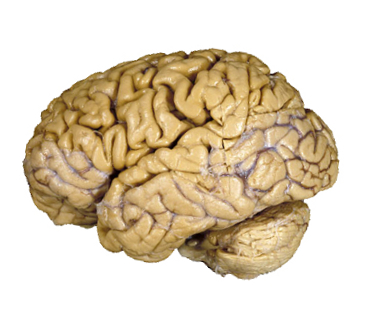
\includegraphics[width=0.3\linewidth]{figures/exvivobrain.jpg} &
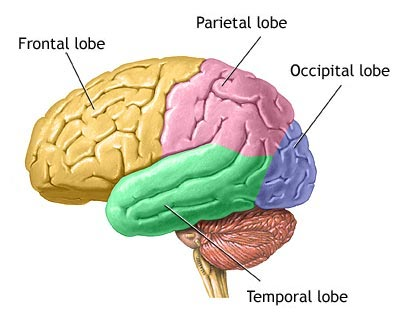
\includegraphics[width=0.3\linewidth]{figures/brainlobes.jpg} &
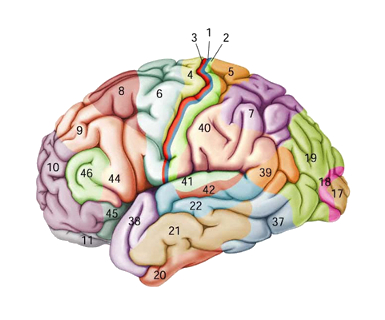
\includegraphics[width=0.3\linewidth]{figures/brodmann.jpg} \\
a) & b) & c)
\end{array}$
\caption{a) An image of an ex-vivo human brain in which the forebrain and hindbrain are visible (image adapted from~\cite{exvivobrain}) b) Each hemisphere of the the forebrain is divided into four lobes as illustrated here (image adapted from~\cite{medlineplus}) c) Brodmann proposed a labeling of the brain surface based upon cytoarchitectural features of the brain (image adapted from~\cite{mcgillbrain})}.
\label{fig:brainanatomy}
\end{center}
\end{figure}

The anatomy of the cerebral white matter is important as it provides the communication network that allows the functional subregions of the cortex to communicate with each other and consists of three types of fibers: (1) projection fibers connect the cortex with the lower parts of the brain and the spinal cord (figure \ref{fig:sketches}a). (2) commisural fibers connect the two hemispheres of the brain (figure \ref{fig:sketches}b). (3) association fibers unite different parts of the same cerebral hemisphere. There are two types of association fibers: (1) those connecting adjacent gyri, short association fibers (i.e.\ u-fibers); (2) those passing between more distant parts, long association fibers. The ability to identify functionally specific subregions of the cortex and the white matter pathways that connect them provides a full anatomical description of specialized neural networks such as the language, memory and visuospatial networks. 

\begin{figure}
\begin{center}
$\begin{array}{ccc}
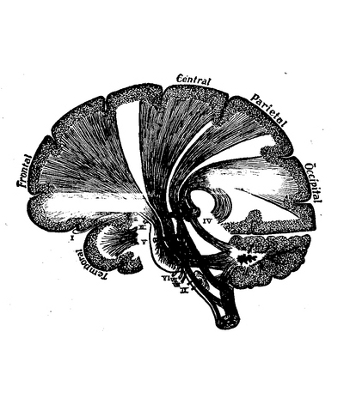
\includegraphics[width=0.3\linewidth]{figures/projectionfiberssketch2.jpg} &
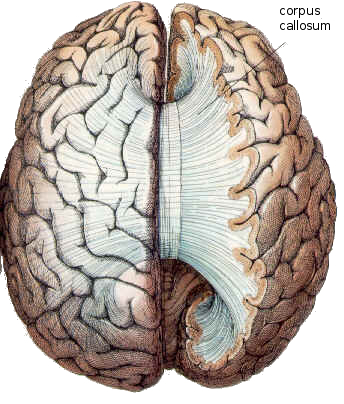
\includegraphics[width=0.3\linewidth]{figures/corpuscallosumsketch.jpg} &
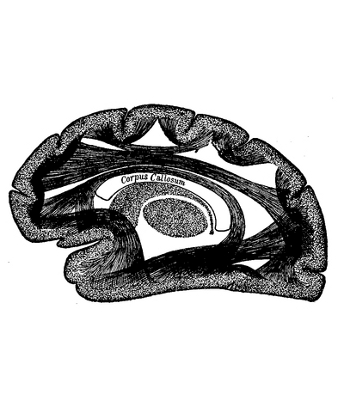
\includegraphics[width=0.3\linewidth]{figures/associationfibersketch2.jpg} \\
a) & b) & c)
\end{array}$
\caption{
Cortical regions communicate via the white matter which consists of: a) the projection fibers that connect the cortex to the lower brain and spinal cord (image adapted from~\cite{gutenberg}) b) The commisural fibers that connect the hemispheres of the brain (image adapted from~\cite{carleton}) c) the association fibers the provide both long and short range intra-hemispheric connections (image adapted from~\cite{gutenberg}).}
\label{fig:sketches}
\end{center}
\end{figure}

\section{Connectivity in the brain}
The human brain is a system comprised of more than $10^{10}$ neurons that provide great computational capacity via a complicated communication network consisting of both local circuits and long-range fiber pathways~\cite{Hagmann2008}. The neurons of the cortical gray matter are responsible for processing information while their axons comprise the white matter that provides the communication channels between the functionally and structurally segregated subregions of the cortex. The study of brain connectivity seeks to understand the anatomical arrangement, structural properties, interconnections, and functional relationships of the elements of this system and is essential for further insight into the nature of cognitive processes and could provide a critical window onto development, aging and neurodegenerative disease in the brain.

\subsection{Anatomical and Structural Connectivity}
The terms anatomical connectivity and structural connectivity are sometimes used interchangeably, but here we distinguish between the two in an attempt to explore the relationship between them as well as the extent to which each relates to functional connectivity. Anatomical connectivity identifies the presence of a physical connection between distinct regions in the brain and quantifies the geometry of the regions and the pathways that connects them. Structural connectivity is concerned with the biophysical properties of the tissue that connects the regions. Collectively, anatomical and structural connectivity are known as the human connectome and they comprehensively describe the biological network of elements that define the human brain~\cite{Hagmann2008}. 

% Anatomic connectivity
Brain development plays an important role in defining the geometry and topography of anatomical connections.
Phylogenetically older brain regions develop first and have direct, sometimes unidirectional, connections~\cite{Gogtay2004b}. The connections typically have a linear configuration as seen in the corticospinal tracts and the thalamo-cortical network. Cortical regions associated with more complex neural networks that require a higher degree of interconnectivity develop later and consist of systems in which subregions may be connected directly or indirectly via intermediary cortical regions. While functional regions of the cortex have been well defined from lesion and functional studies, white matter connective pathways are not as clearly defined due to these indirect and parallel connections. This can lead to confusion and ambiguity regarding the components that comprise a particular neural network. A greater understanding of the inter-relations between anatomy and function in the brain could help identify the components that are relevant to a functionally specific network.

%Structural Connectivity
Structural connectivity examines the architectural properties of anatomical connections in order to estimate the integrity or efficacy of the connections. As with anatomic connectivity, brain development plays an integral role in defining structural connectivity. In addition to temporal variance of maturation, white matter also exhibits spatial variation with maturation first occuring centrally and then peripherally, and from the occipital lobe to the frontal lobe~\cite{Gao2009}. The myelin sheath that surrounds the axons of the white matter provides insulation that enhances the speed at which signals are transmitted by the fibers. Degree of myelination provides the basis for many meaures of structural integrity and the spatial arrangement of myelin sheaths provides a basis for elucidating fiber orientation.

Gall and Spurzheim~\cite{Gall1810} were the first to establish that white matter consists of individual fibers that are grouped into tracts that provide a biological connection between cortical gray matter regions. The myelin sheath that surrounds axons was first described by Thomas Schwann~\cite{McHenry1969}, but the term `myelin' itself was introduced later by neuropathologist Rudolph Vircho~\cite{Morell1980}. Carl Weigert's development of a histological stain for the identification of myelin was critical to advancing the study of white matter and is still is use today~\cite{McHenry1969}. Further work in histological staining techniques by Camillo Golgi provided the ability to visualize entire nerve cells, including the dendritic tree~\cite{Golgi1885}. This technique was employed extensively by Santiago Ram{\'{o}}n y Cajal to study nerve cells in the brain and spinal cord~\cite{Glickstein2006}. The work of Paul Flechsig (1847-1929) greatly advanced knowledge regarding white matter as he was the first to observe that myelination during development varied based upon anatomical location and he also introduced Flechsig' rule, stating that cortical sensory areas are not directly connected with each other, but rather connect to adjacent association cortices~\cite{Flechsig1901}, a concept that profoundly influenced modern neuroscientific concepts related to cortical localization. The development of horseradish peroxidase (HRP) tract-tracing allowed for the precise identification of neural pathways in ex-vivo~\cite{Mesulam1982}. More recently, magnetic resonance imaging (MRI) has allowed for routine imaging of gray and white matter and these methods are discussed in more detail in chapter 2. 

\subsection{Functional Connectivity}
The functional organization of the brain seems to obseve two guiding principles: functional segregation and functional integration~\cite{Tononi1994}. Functional segregation refers to the organization and grouping of functionally specialized neurons into spatially distinct cortical brain regions. However, in order to perform complex tasks it is necessary for several functionally segregated and anatomically distinct regions to work together and form functional networks under a concept known as functional integration. Further understanding of brain function requires not only knowledge about the functional topography of the brain but also the complex processes by which these regions interact. Functional segregation and integration and both central to the study of functional connectivity. Functional connectivity has been refered to as an `elusive concept' due to the large variety of defintions, modalities and methods that have been described using this term~\cite{Horwitz2003}. Here we will reserve the term `functional connectivity' to refer to statistical paradigms that identify temporally coordinated activity in spatially distinct units within an individual's brain~\cite{Rykhlevskaia2008}.

Early work examining Gall's theory of functional segregation focused upon cortical lesion studies. In particular, the work of Paul Broca (1824 - 1880) provided evidence for the localization and lateralization of language procesing through post-mortem autopsy of patients who had been unable to pronounce individual words but were unable to produce grammatically correct sentences, a condition later named ``Broca's aphasia." Further work in the language system by Karl Wernicke (1848 - 1905) recognized that not all language deficits resulted from lesions in the cortical region identified by Broca. Through lesion analysis Wernicke identified a cortical region that when damaged prevented subjects from speaking, but did not impede their ability to understand language. The proposal that multiple functionally specific cortical regions work together to perform complex tasks is the basis of functional integration. Additionally, this proposal predicted the importance of structural connectivity as it recognized the critical role of the biological connections between functional regions. Norman Geschwind (1926 - 1984) expanded upon Wernicke's model of the language network and theorized the existence of a parallel pathway connecting Broca's and Wernicke's areas that incorporates an additional cortical region. More recently, additional evidence for functional segregation has been provided by a variety of techniques including PET~\cite{Zeki1991}, electrophysiology~\cite{Gevins1999} and functional MRI (fMRI)~\cite{Howard1996}. Neuroimaging continues to be used extensively to study functional integration and functional connectivity~\cite{Sporns2007B} and these methods are discussed in more detail in chapter 2.

%\subsection{Effective Connectivity}
%Effective connectivity is defined as `the influence that one neural system exerts over another either directly or indirectly'~\cite{Friston1993}. Studies of effective connectivity utilize methods that employ statistical models and make anatomical assumptions to restrict the analysis to a subset of functional regions. The incorporation of anatomical assumptions provides an opportunity for a combined analysis of functional, anatomical and structural connectivity. Unlike functional connectivity measures that attempt to measure what the brain is doing, effective connectivity examines how the brain is working. Studies of effective connectivity rely upon neuroimaging methods and chapter 2 reviews the approaches that have been proposed for modeling the dynamics of cortical circuits.

%First developed for use in econometrics, structural equation modeling (SEM) has been applied to the study of effective connectivity~\cite{McIntosh1994}. These models incorporate directed connections between cortical regions to ascribe causal relationships. Two major limitations of SEMs are the (1) reliance upon correlations matrices that limits the number of connections and (2) inability to incorporate temporal information. To address these deficiencies, dynamic causal models (DCM) were proposed by Friston, et al.\ \cite{Friston2003}. The causal model utilised in DCMs allow for interregional and self connections that results in changes in blood flow, volume, and deoxyhemoglobin (dHb) content. These parameters, all of which contribute to the BOLD fMRI signal, are quantified by DCM.  DCM is currently limited by the computationally demanding model fitting that limits the analysis to small number of regions.


\section{Introduction to the dissertation}

Here we present novel approaches for examining connectivity in the brain. We focus on connectivity at the macro scale and how it may be studied with MRI. To this end, we use diffusion tensor MRI along with fiber tractography to extract anatomical and structural information from white matter fiber bundles. We demonstrate the ability of these methods to identify both local and gross white matter properties. Atlas-based techniques are used to define geometric models of white matter fiber pathways. These models are used to identify the white matter fiber tracts that provide the anatomical connectivity that provides communication between the nodes of a functional network defined using fMRI. Meaures of structural and functional connectivity are related to cognitive performance in a language-based decision making task. 

Chapter~\ref{chap_back} presents background on methods for using neuroimaging to study connectivity in the human brain.  Chapter~\ref{chap_tbi} focuses on using fiber tractography to examine an a priori functionally-based hypothesis regarding localized structural differences in a population of subjects whom have suffered a traumatic brain injury (TBI). Chapter~\ref{chap_homo} describes an examination of both structural and functional connectivity in a healthy young adult population and relates these measures to cognitive performance. In chapter~\ref{chap_lat} we discuss a study of lateralization in the brain and examine the influence of aging on both structure and function. Finally, in chapter~\ref{chap_conclusions}, we discuss the findings described in this dissertation and interesting questions to be investigated in the future.

%Chapter 3 dicusses the use of fiber tractography for examining the topography of inter-hemispheric cortical connectivity and evaluates schemes for anatomical connectivity based partitioning of the mid-sagittal cross-section of the corpus callosum.

%The anatomical frame-of-reference provided by the fiber model is used to develop metrics that incorporate the  eometry of the model and quantify how it related to the underlying structure in individual subjects. 
%We demonstrate the ability of these methods to identify both local and gross white matter differences and characterize difference types of connective pathologies and the metrics appropriate for their investigation. Finally, a healthy control atlas is used to model the language network in order to explore the relationship between functional and structural connectivity in a well-known sub-network of the brain and demonstrate how they may be used to identify the most likely candidate when multiple network configurations are possible. Performance in a task-based functional experiment is used to characterize the contributions of the different types of connectivity to cognitive performance.



%
%
%
% From proposal
%
%
%


%Paragraph discussing brain as a computational network


% DTI and structural connectivity
%\section{Diffusion Tensor MRI}
%Of particular interest in this work is the use of diffusion tensor MRI in the examination of structural connectivity. Diffusion tensor imaging provides an \emph{in-vivo} non-invasive measure of the local probability of self-motion of water molecules and has proven useful in a number of applications for the study of brain white matter~\cite{Basser1994}. 
%The diffusion of water in white matter is highly anisotropic due to cell walls and myelin which inhibit diffusion perpendicular to the fiber tracts more so than diffusion parallel to the tracts. Both the shape and orientation of the diffusion tensor provide important information regarding the structure of the white matter. Scalar metrics derived from the diffusion tensor, such as fractional anisotropy (FA) and mean diffusion (MD) are often used to quantify various tissue properties. The structural information provided by the diffusion tensor has been shown to be useful in a multitude of studies examining topics such as neurodegenerative disorders, traumatic brain injury, development, and ageing among others~\cite{Lebel2008,Sydykova2007,Xu2007}.


%\section{Structural Connectivity}
%Recently, a number of studies have sought to use DTI to measure whole brain structural connectivity~\cite{Honey2009,Hagmann2008,Hagmann2007,Sporns2005,Iturria-Medina2007}. Many of these studies have relied upon measures such as "fiber counts" and fiber length to estimate structural connectivity. These types of metrics are known to be unreliable due to bias resulting from total brain volume, differences in size between regions of the brain, noise, and partial voluming~\cite{Corouge2006}. Additionally, they fail to incorporate the geometric features provided by the tract model as well as neglecting to incorporate the biophysical properties of the tissue that compromises these fiber pathways. The use of metrics for structural connectivity that leverage the anatomic framework provided by tractography to probe underlying tissue architecture may provide more relevant insight regarding the physical integrity of cortical connections. 

%The examination of cortical thickness provides an alternative method for examining structural connectivity between cortical regions~\cite{Lerch2006,He2007,He2008}. This approach is similar to methods for examining functional connectivity where a seed region-of-interest is used to test for statistical dependence with other point in the cortex. Here however, measures of cortical thickness are compared. An examination of the language network revealed a connectivity pattern that closely resembles the results of fiber tractography studies~\cite{Lerch2006} and a study of Alzeheimer's disease provided evidence of large-scale disruption of integrity in brain networks~\cite{He2008}.

%%Paragraph discussing graph based analysis of the brain network
%\section{Graph-based Analysis of Connectivity}
%The use of graph-based network analysis techniques provides a natural, and increasingly popular, framework for examining connectivity in the brain~\cite{Hagmann2007,Iturria-Medina2007,Iturria-Medina2008,Hagmann2008,Honey2007,Achard2006}. The vertices of the graph correspond to functionally related sets of neurons while the edges correspond to the physical connection or statistical dependencies between these nodes. Much previous work used this concept to study functional connectivity but recently a great deal of work has focused upon incorporating both structural and functional connectivity into a common network for analysis~\cite{Werring1998a,Werring1999b,Wieshmann2001,Honey2009,Bullmore2009,Koch2002a,Skudlarski2008}. Vertices may interact via multiple connections with variable length or weights assigned to them as well as through indirect paths that pass through other vertices. This representation provides a multitude of methods for examining the data such as clustering, path lengths, vertex degree and strength and many others~\cite{Brandes2005}. This framework additionally provide a natural basis for examination at multiple scales. 

%% How we address the above work with novel work
%\section{Significance of Proposed Work}
%Here we present  a framework for examining connectivity in the brain. We focus on connectivity at the macro scale and how it may be studied with MRI. To this end, we using diffusion tensor MRI along with fiber tractography to extract structural information from white matter fiber bundles. The anatomical frame-of-reference provided by the fiber model is used to develop metrics that incorporate the geometry of the model and quantify how it related to the underlying structure in individual subjects. 
%We demonstrate the ability of these methods to identify both local and gross white matter differences and characterize difference types of connectivity pathologies and the metrics appropriate for their investigation. Finally, a healthy control atlas is used to model the language network in order to explore the relationship between functional and structural connectivity in a well-known sub-network of the brain.















% Background and Significance
% No page limit
\chapter{Background: Neuroimaging for the Examination of Anatomy, Structure and Function in the Human Brain }
\label{chap_back}

The modern development of methods for in-vivo imaging of the human brain is indispensable for understanding of brain function and malfunction. While techniques such as positron emission tomography (PET) provide the ability to image brain activation, the significantly better spatio-temporal resolution provided by magnetic resonance imaging (MRI) has made it the technique of choice for identifying anatomy and in studies of both structure and function in the brain. Different tissue types are distinguished by MRI based upon the levels of hydrogen that they contain. Because white matter contains a large amount of tissue, while gray matter has many fluid-containing cell bodies, MRI is particularly good for distinguishing between these tissue types. The versatility of MRI has led to the development of techniques to measure structure and function in the brain, providing a framework for examining the relationship between structural and functional connectivity and their role in modulating behavior.

% DTI
\section{Diffusion Tensor MRI}
Of particular interest in this dissertation is the use of diffusion tensor MRI in the examination of structural and anatomical connectivity. Diffusion tensor imaging provides an in-vivo non-invasive measure of the local probability of self-motion of water molecules and has proven useful in a number of applications for the study of brain white matter~\cite{Basser1994}. The diffusion of water in white matter is highly anisotropic due to cell walls and myelin which inhibit diffusion perpendicular to the fiber tracts more so than diffusion parallel to the tracts. Both the shape and orientation of the diffusion tensor provide important information regarding the structure of the white matter. Scalar metrics derived from the diffusion tensor, such as fractional anisotropy (FA) and mean diffusion (MD) are often used to quantify various tissue properties. The structural information provided by the diffusion tensor has been shown to be useful in a multitude of studies examining topics such as neurodegenerative disorders, traumatic brain injury, development, and aging among others~\cite{Lebel2008,Sydykova2007,Xu2007}.

\subsection{Diffusion weighted MRI}
% Molecular Diffusion
The constant random motion of particles in liquids, known as Brownian motion, provides a method for using MRI to measure the self-diffusion of water.  As the particles move they collide with other particles and over time the path of any given particle may be described by a random walk.  In the presence of a concentration gradient, a flux of the fluid is observed.  If no concentration gradient is present it becomes necessary to describe diffusion as the statistical probability that a particle moved a certain distance in a given time.  Einstein~\cite{Einstein} showed that such a probability has a zero-mean Gaussian distribution with a variance that is proportional to time:
$$ <r^2> = 2NDt, $$
where $D$ is the diffusion coefficient, $t$ is time, and $N$ is the number of spatial dimension over which distances are measured.

% Measuring Diffusion with MRI
In the case of MRI, diffusion may only be measured in one direction at a time, so $N$ is equal to one.  As spins in the presence of a magnetic field gradient diffuse, they accumulate phase shifts, thus reducing the intensity of the MR signal.  This effect may be magnified with the use of stronger gradients, and may be accurately measured with a spin-echo sequence such as the one illustrated in Figure~\ref{fig:sequence} that includes equal rectangular gradient pulses both before and after the refocusing pulse.  During the first pulse, spins acquire different phase shifts based upon their location.  If the spins remain stationary, then these phase shifts are reversed during the second pulse.  Spins that diffuse however will acquire a net phase shift resulting in a signal attenuation, $A$, that is proportional to the diffusion coefficient, $D$, according to
\begin{equation}
\label{eq:attenuation1}
A = e^{-bD}
\end{equation}
where $b$ is the 'b-factor', a quantity characterized by the amplitude, shape, and timing of the magnetic field gradient used for acquisition.

\begin{figure}[ht]
\begin{center}
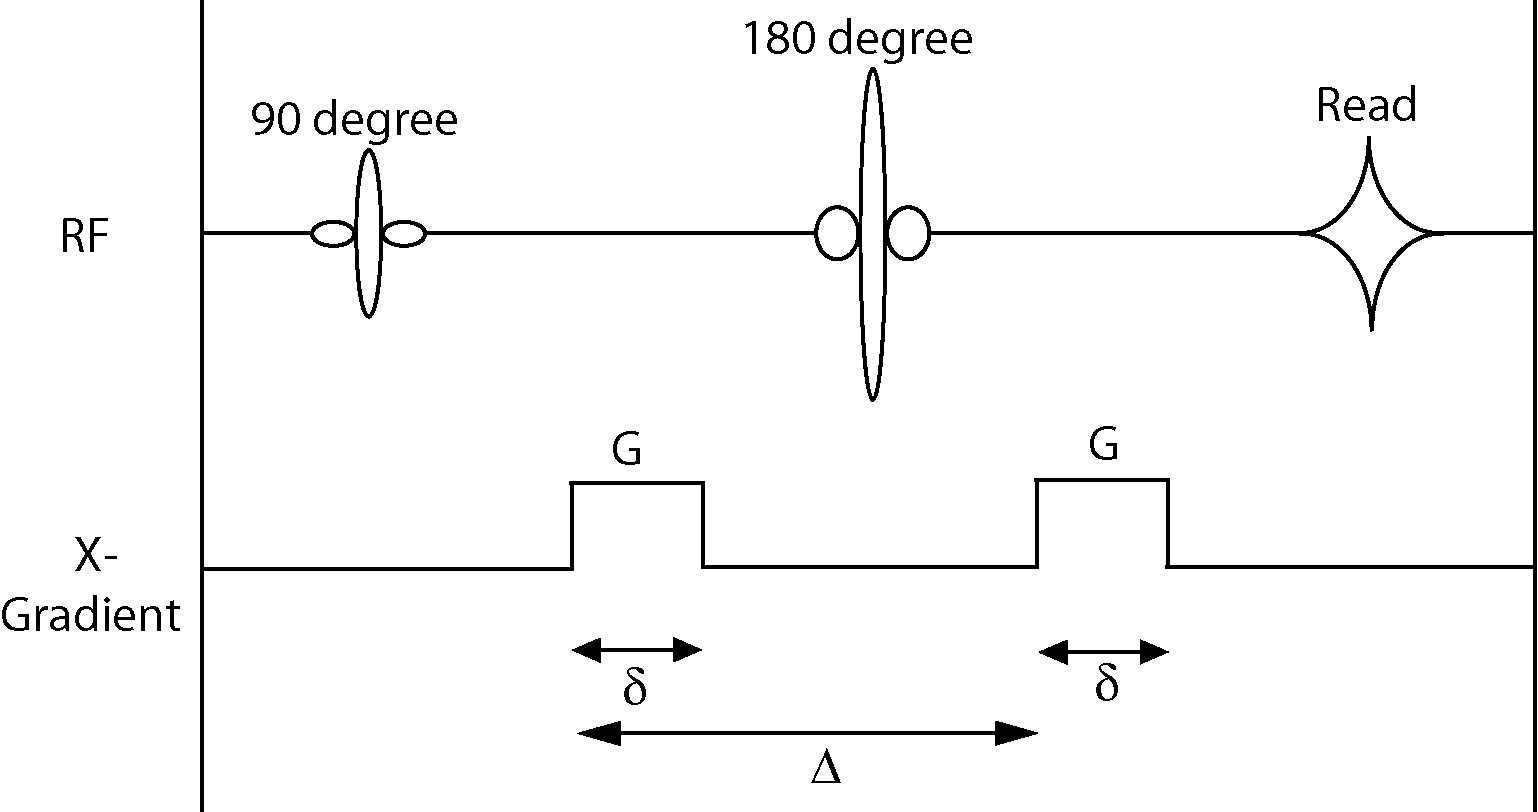
\includegraphics[width=4in]{figures/sequence}
\caption{
\label{fig:sequence}
An example diagram of a Stejskal-Tanner pulse gradient spin echo experiment used to measure diffusion (adapted from ~\cite{Behrens2004}).  For further explanation on understanding pulse sequence diagrams, please see \cite{Haacke}.}
\end{center}
\end{figure}

% Measuring the Tensor
\subsection{Measuring the diffusion tensor}
In the case of isotropic tissue, diffusion may be described by a single scalar parameter, the diffusion coefficient.  However, tissue such as white matter is anisotropic and in order to fully characterize the diffusion it is necessary to use a tensor which describes diffusion along each direction and the correlations between these directions \cite{LeBihanJMRI2001}.  Mathematically, a symmetric, second order tensor, $D$, is used to describe the three dimensional self-diffusion of water within a volume:
$$ \underline{D} = \begin{pmatrix} 
	D_{xx} & D_{xy} & D_{xz} \\
	D_{yx} & D_{yy} & D_{yz} \\
	D_{zx} & D_{zy} & D_{zz}
	\end{pmatrix}
$$
The principle directions of diffusivity may be used to define a reference frame [$x', y', z'$] .  In this case, the diagonal terms of the tensor, $D_{x'x'}, D_{y'y'}, D_{z'z'}$, may be used to represent diffusion along [$x', y', z'$] and the attenuation becomes
\begin{equation}
\label{eq:attenuation3}
A = e^{-b_{x'x'}D_{x'x'} - b_{y'y'}D_{y'y'} - b_{z'z'}D_{z'z'}}
\end{equation}
where $b_{ii}$ are elements of the b matrix which expresses the b-factors for the directions in the reference frame.  However, measurements are actually made in a frame of reference [$x,y,z$] defined by the scanner.  This makes it necessary to incorporate the non-diagonal elements of the \underline{b} matrix in order to incorporate the correlation of diffusion in perpendicular directions, leading to
\begin{equation}
\label{eq:attenuation6}
A = e^{- \sum_{i=x,y,z}{ \sum_{i=x,y,z}{ \underline{b}_{ij}\underline{D}_{ij} } } }
\end{equation}
Because the diffusion tensor is symmetric, $D_{ij} = D_{ji}$, the attenuation may also be written as
\begin{equation}
\label{eq:attenuationfull}
A = e^{-b_{xx}D_{xx} - b_{yy}D_{yy} - b_{zz}D_{zz} - 2b_{xy}D_{xy} - 2b_{xz}D_{xz} - 2b_{yz}D_{yz} }
\end{equation}
In order to determine the diffusion tensor it is necessary to obtain six or more measures of attentuation, which requires a minimum of six diffusion weighted images and one non-diffusion weighted image.
  
The eigensystem of $D$ consists of three eigenvectors, $e_1, e_2, e_3$ and their corresponding eigenvalues $\lambda_1  \le \lambda_2 \le \lambda_3$. The eigenvectors describe the principal axes of diffusion, and the eigenvalues are proportional to the mean squared displacements along the corresponding eigenvector. The values may be used to define visualization of tensor such as ellipsoids with orientation determined by eigenvectors and size determined by eigenvalues. The mapping of the components of $e_1$ into an RGB-color space is known as a directionally encoded color (DEC) map~\cite{Pajevic1999}.
  
\begin{figure}[ht]
\begin{center}
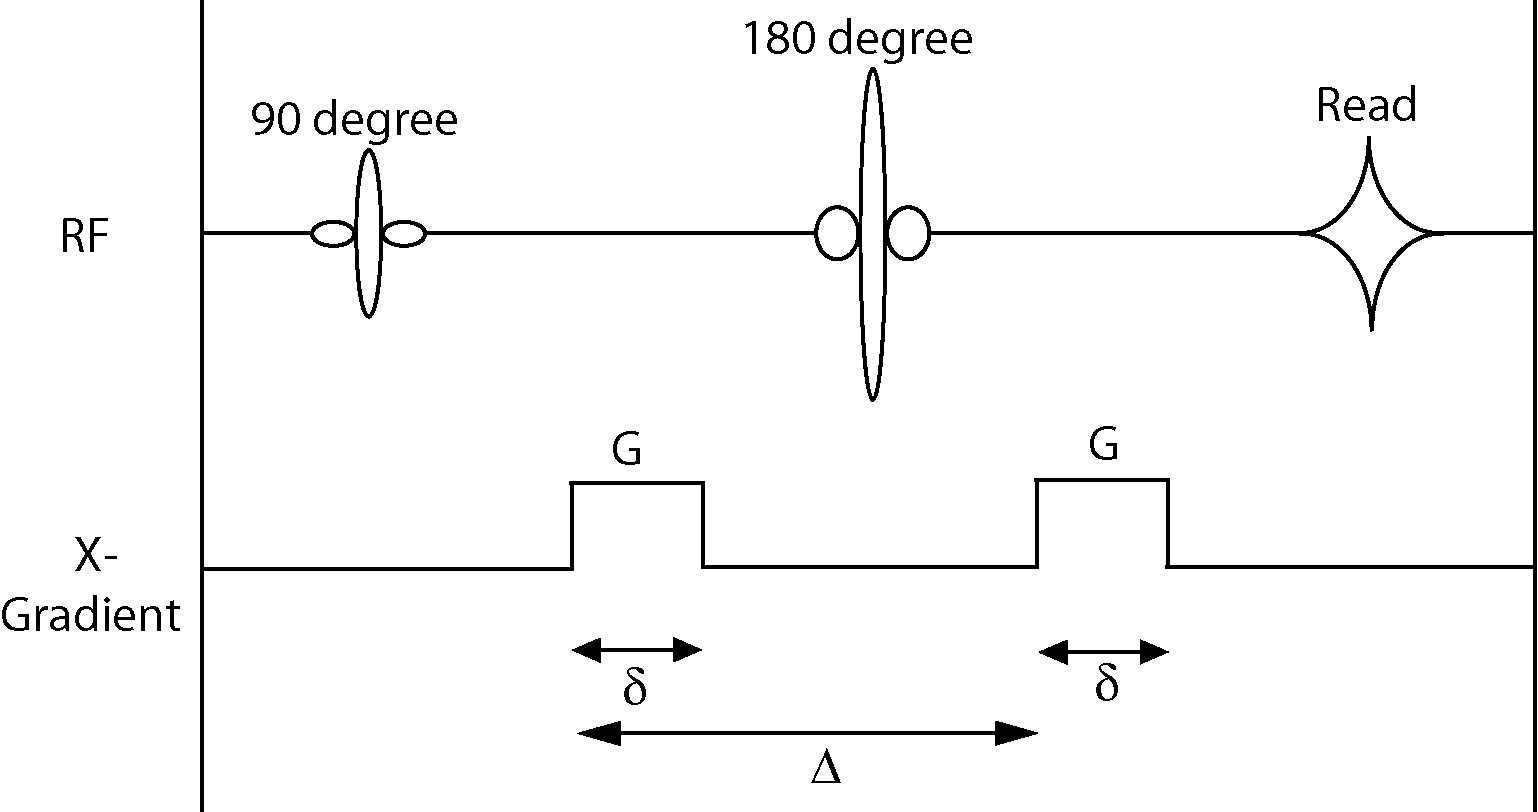
\includegraphics[width=4in]{figures/sequence}
\caption{
\label{fig:sequence}
An example diagram of a Stejskal-Tanner pulse gradient spin echo experiment used to measure diffusion (adapted from Behrens thesis).  For further explanation on understanding pulse sequence diagrams, please see \cite{Haacke}.}
\end{center}
\end{figure}
  
% Diffusion in fibrous tisssue
In tissue, the diffusion of water may be anisotropic, i.e. it may vary with direction, due to the presence of obstacles that limit molecular movement.  The axons of white matter are insulated with a fatty protein called myelin which insulates the the axon improves the efficiency of signals that travel along the axon~\ref{fig:neuron}. In fibrous tissue such as white matter the arrangement of nerve fibers into bundles results in a bias in which diffusion parallel to the fibers is often 3-6 times faster than diffusion perpendicular to the fiber bundle \cite{LeBihanNATURE2003} due to the restriction of water diffusion caused by myelin and the cell walls of the axons.  This ability to estimate fiber bundle orientation within a voxel led to the field of fiber tractography.  

\begin{figure}[ht]
\begin{center}
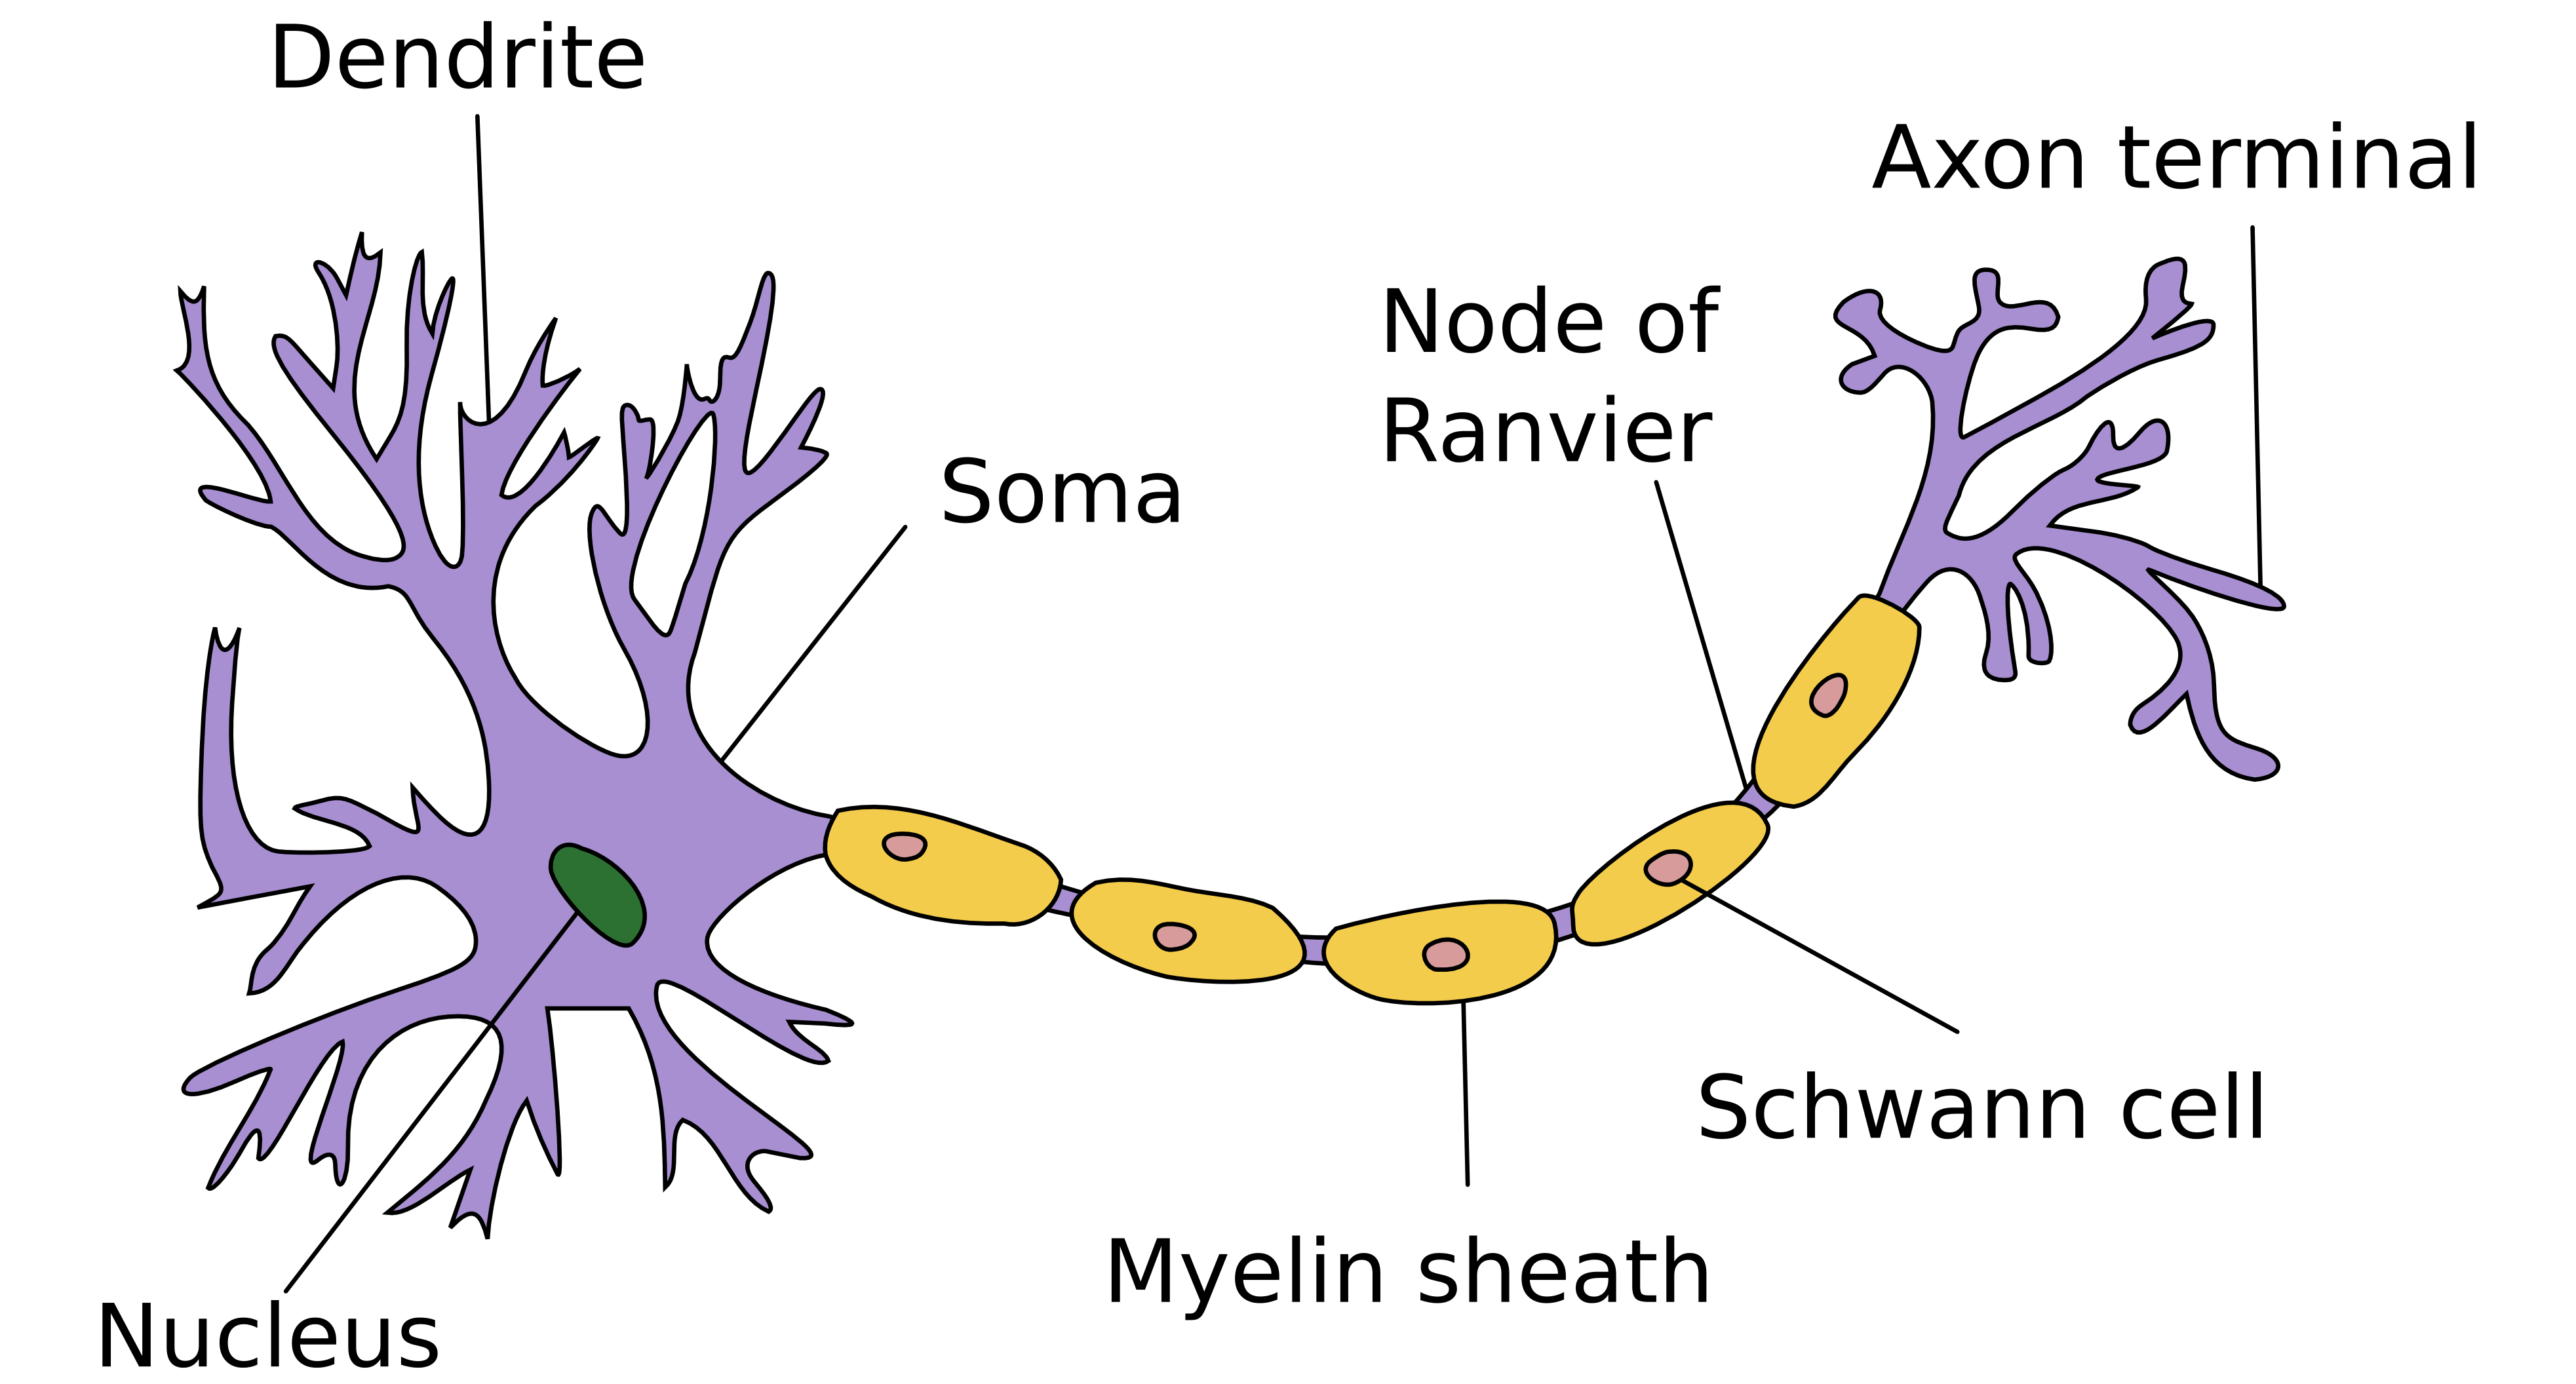
\includegraphics[width=0.75\linewidth]{figures/Neuron_Hand-tuned.png}
\caption{
\label{fig:neuron}
Diagram on a neuron with a myelinated axon (adapted from wikipedia).}
\end{center}
\end{figure}

\subsection{Fiber tractography}
A great deal of research focused upon methods for fiber tractography which use the fiber orientation information provided by the diffusion tensor to estimate trajectories of white matter fiber bundles throughout the brain. Tractography may provide a framework for identifying anatomical connections and studying the structural properties of the underlying white matter. Tractography methods can be grouped into 3 categories: deterministic, probabilistic, and energy-minimizing. 

\subsubsection{Deterministic tractography}
Deterministic tractography methods use a starting seed point, and then the direction information provided by the diffusion tensor is used to trace fiber trajectories until the end of a fiber bundle is reached~\cite{Basser2000,Mori99b}. These trajectories are referred to as streamlines. Due to the limited spatial resolution of DTI, streamlines represent estimated pathways of large bundles of fibers and do not correspond to the trajectories of individual axons. Methods for deterministic tractography typically differ in the details of the methods used to infer fiber direction from the underlying tensor field. Approaches include following $e_1$ from voxel to voxel~\cite{Mori1999}, linear interpolation of $e_1$ combined with a fixed step-size~\cite{Conturo1999}, linear interpolation with adaptive step-size using the Runge-Kutta method~\cite{Basser2000,Tench2002}, and methods that incorporate a momentum term to account to account for previous steps~\cite{Lazar2003}. To determine when then end of a fiber bundle has been reached, various stopping conditions are used such as FA thresholds~\cite{Conturo1999}, local curvature thresholds~\cite{Basser2000}, and measures of local orientation dispersion~\cite{Mori1999}

All deterministic methods suffer from error propagation resulting from noise in the DTI signal~\cite{Basser2000}. The extent of the error varies with the geometry of the fiber bundle, the anisotropy in the white matter, the resolution of the data, and the interpolation method~\cite{Lori1999}. Deterministic method may fail when a single voxel contains fibers from two or more distinct populations including fiber that cross, ``kiss", branch or merge~\cite{Basser2000}. One approach to avoid false-negative connections is a brute-force approach to seed selection known as whole-brain tractography. In this approach, all points in the brain are used as seeds for fiber tractography~\cite{Conturo1999}.
A lack of confidence measures for streamlines makes the automatic identification of spurious streamlines difficult. The use of user defined landmarks may reduce this problem but is time intensive and requires exiting knowledge of anatomy~\cite{Mori2002a,Wakana2004,Wakana2007}.

\subsubsection{Probabilistic tractography}
Probabilistic tractography methods use the fiber orientation measurements provided by diffusion weighted MRI to estimate the likelihood of a connection between two points. This likelihood is the integral of all possible paths that connect two points and is solved analytically by generating a set of ``probabilistic streamlines". At each point in the image, a local probability density function (PDF) of orientation is defined. A probabilistic streamline is traced by drawing a sample orientation from the PDF at each point and advancing by a small step along that direction. As with deterministic tractography, this advancement continues until a stopping criteria determines that the end of the fiber bundle has been reached. A final measure connectivity between two points is then determined by calculating the probabilistic index of connectivity (PICo), a quantity that was introduced independently by Parker et al.\ \cite{Parker2002} and Lazar and Alexander~\cite{Lazar2003}. Approaches to probabilistic tractography differ in the approach to estimating the PDF which include model-based approaches~\cite{Parker2002,Lazar2003} and a Bayesian approach~\cite{Behrens2004}. 

Model-based approaches to estimating the PDF are limited by the sources of uncertainty that may be included in the model. Uncertainty resulting from patient motion and eddy-current distortion are not included in the estimates of uncertainty. Additionally, these methods assume a Gaussian diffusion of water which is not necessarily the case. Probabilistic tractography methods are also sensitive to seed selection. Because a large number of streamlines are calculated for each seed (typically near 10,000) the whole-brain approach used in deterministic tractography may not be a practical option for examining human data. 

\subsubsection{Energy-minimizing tractography}
Energy-minimizing tractography approaches may be grouped into two categories, fast-marching and simulated annealing. Fast-marching methods rely upon level-set theory and the fast-marching algorithm. From a given seed point, the speed and direction of a propagation front are defined from local tensor properties. The use of local properties means that the propagation of the front will vary in different regions of the brain. Time-of-arrival maps are then determined for the whole brain and used to estimate the likelihood of a connections between a seed and any given point in the brain. These methods differ in the details of how the tensor data is used to define a speed and direction of the propagation front. Parker et al.\ \cite{Parker2002a} relied upon $e_1$ while O'Donnell et al.\ \cite{ODonnell2002} incorporated the whole diffusion-tensor. The simulated annealing approach considers two points, and attempts to identify the most favorable path that connects these points. Local energies at points along a potential path are determined based upon geometric properties of the path (short, straighter paths are generally preferred) and upon agreement between the direction of the path and the orientation of the underlying tensor field. Energy-minimizing methods differ in the details of how a local energy is determined~\cite{Tuch2000,Tuch2001}. Energy-minimizing approaches rely upon a priori knowledge of anatomy as they require the selection of two end points to examine. False-positive connections are also a problem as these methods are guaranteed to fine some level of connectivity between any two points, even when that connection is not anatomically feasible. While these methods present potential solutions to the problems caused by fiber crossing and branching, little has been done to evaluate the methods or demonstrate their performance in clinical data.

%fMRI
\section{Functional MRI}
Brain activation may be mapped with MRI by exploiting the interrelationship between physiological function, energy metabolism and localized blood supply. In particular, the blood-oxygenation-level-dependent (BOLD) contrast mechanism first demonstrated by Ogawa, et al.~\cite{Ogawa1990}, has been employed extensively due to its high sensitivity and accessibility. The BOLD contrast results from gradient echo techniques that accentuate the susceptibility effects of deoxyhemoglobin (dHb) in the venous blood and thus reflects the blood oxygen level. While increased neural activity should result in a decreased BOLD signal due to field inhomogeneities caused by dHb, brain activation causes an increased BOLD signal due to increased cerebral blood flow that is not balanced by a commensurate increase in oxygen consumption rate~\cite{Fox1986} thus resulting in lower dHb content per volume of tissue. Additional research has revealed the BOLD contrast to be the complex result controlled by many parameters. Despite this complexity, the BOLD signal has been successfully used in hundreds of studies of human brain as well as a large number of animal studies.

\subsection{Functional connectivity}
The use of BOLD fMRI for mapping human brain function has seen widespread use for the past two decades. While earlier research focused upon the identification of activated brain regions, more recently increased attention has been paid to the examination of the interactions and coordination between different parts of the brain~\cite{Fox2005,Greicius2003,Munk2002}. Specifically, studies of functional connectivity seek to identify `temporal correlations between spatially remote neurophysiological events'~\cite{Friston1993,Lee2003}. Here we focus on methods for the study of functional connectivity related to neurophysiological events as opposed to methods designed to examine resting state functional connectivity. These methods may be grouped into two categories, model-based methods that incorporate a priori knowledge and data-drive methods that that not require any prior knowledge.

\subsubsection{Model-based functional connectivity}
Model-based methods generally rely upon seed regions that defined using prior anatomical knowledge. A metric of similarity is defined in order to generate connectivity maps and a number of metrics have been proposed. Cross-correlation analysis (CCA) has been used extensively since it's introduction for use in functional connectivity by Cao and Worsley~\cite{Cao1999}. This method measures correlations in the fMRI time-signals and may include the entire time-course or only time points that correspond to a stimulus of interest. Additionally, CCA may examine correlations at different time lags, though many studies only examine the zero lag scenario. CCA is susceptible to artifacts caused by cardiac activity and blood vessel activity that may result in false-positive identification of correlations~\cite{Friston1995}. Coherence analysis was introduced by Sun et al.\ \cite{Sun2004} to try to address these shortcomings. Coherence analysis is the spectral representation of correlation in the frequency domain, a conversion that provides a natural framework for comparing time signals. The requirement of seed-selection limits these studies to the examination of cortical regions that have been selected via prior knowledge~\cite{Ma2007}. Additionally, these methods typically only examine additional regions identified via prior and neglect to examine other brain regions. While these methods are useful in the examination of systems defined by strong prior knowledge, they do not provide the ability to fully explore functional connectivity throughout the brain.

\subsubsection{Data-driven functional connectivity}
To overcome that need for prior anatomical knowledge that is required for model-based techniques, data-driven techniques were developed, allowing for explorative studies of whole brain functional connectivity. Principle component analysis (PCA) is a widely used technique and was introduced for functional connectivity analysis by Friston et al.\ \cite{Friston1993}. In PCA, the fMRI time-signals are represented by orthogonal contributors in order to identify the vectors that most contribute to variance. These methods have trouble identifying functional connectivity in the presence of physiological noise~\cite{Baumgartner2000} and are often used as a precursor to independent component analysis (ICA). ICA is similar to PCA but identifies components that are as statistically independent as possible~\cite{Hyvaerinen2000} and was introduced into use for functional connectivity by McKeown et al.\ \cite{McKeown1998}. Despite the wide use of ICA methods, there are still no clear guidelines indicating when the data should be decomposed into spatially or temporally independent components. Both ICA and PCA provide connectivity maps, but the question of how to appropriately threshold these maps is still an open issue~\cite{Ma2007}. 

%\section{Effective Connectivity}

\section{Early neuroimaging studies of brain connectivity}
Extensive progress in neuroimage analysis techniques has resulted in a variety of approaches to examining connectivity in the brain. At the most fundamental level, these techniques are typically categorized into either studies of structural connectivity, functional connectivity, or combined studies of both. Here we provide a review of techniques in each of these categories that are relevant to the work presented here.

\subsection{Structural connectivity}
The study of structural connectivity typically focuses upon the examination of the myelinated axons that makeup white matter. Changes within white matter properties play an crucial role in brain aging~\cite{Abe2008,Allen2005,Bartzokis2004,Kochunov2007,Salat2005a,Salat2005,Walhovd2005,Wozniak2006,Westlye2009}. Additionally, the structural integrity of white matter has been shown to influence cognitive function in both health~\cite{Wolbers2006,Johansen-Berg2007,Tuch2005,Hoeft2007,Floel2009} and disease~\cite{DeCarli1995,Groot2001,Wessels2007,DuFouil2009}. Measures of structural connectivity may also be inferred by measuring the size of white matter structures, an approach that has been used extensively to study the mid-sagittal cross-section of the corpus callosum~\cite{Witelson1989,Colcombe2005a,Gunning-Dixon2000}. Volumetric analysis of white matter fiber tracts has been interpreted as measures of structural integrity~\cite{Salat2005a} and has been used to examine hemispheric asymmetry~\cite{Catani2007,Propper2010}. However, a detailed characterization of the relationship between white matter anatomy and microstructure is still lacking for both health and disease and is an active topic of research. In middle-age, FA has been shown to be more sensitive than white matter volume to changes in white matter integrity, likely due to myelin reduction with increasing age~\cite{Fjell2008}. Additionally, the finding of a weak correlation between FA and white matter volume suggests that these metrics are sensitive to different characteristics of white matter~\cite{Fjell2008}. Correlations have been found between FA and voxel-based morphometry in select fiber tracts such as the corpus callosum and corona radiata~\cite{Hugenschmidt2008}. However an aging study examining FA and white matter volume found that FA correlated negatively with age, but white matter volume did not correlate with age~\cite{Abe2008}. These results suggest that while anatomical based measures and microstuctural based measures of white matter integrity are related, they are complementary and each provides a unique window onto the complex nature of white matter integrity.

A great deal of research into structural connectivity has focused upon methods that incorporate fiber tractography. Identifying the cortical regions to which these fiber bundles extend provides the ability to examine the topography of specific white matter pathways~\cite{Behrens2003}. A typical use of fiber tractography is for defining a region-of-interest by labeling all voxels that contain fibers for the tract of interest and then performing standard ROI analysis. Work exploring the use of fiber-tract oriented statistics presents methods for examining tract-features over the length of tracts~\cite{Jones2005,Corouge2006,Maddah2008d,Lin2006,ODonnell2009,Davis2009,Goodlett2009a,Batchelor2006}, but the identification of appropriate metrics and methods for statistical comparison is still an open issue. The use of template, or representative, fibers is an active topic of research and is sometimes referred to at tract-based morphometry~\cite{O'Donnell2009}, but there currently exists little consensus regarding the "best-practices" for this type of study. Despite the large number of methods available for estimating white matter trajectories, little has been done to rigorously characterize the differences between these methods or define the hypotheses for which they are appropriate, although a study of reproducibility in tract-based studies suggests that the reliability of fiber tractography methods is of central importance to tract-based studies~\cite{Ciccarelli2003}. 

The use of DTI in tract-based studies has received much attention recently~\cite{Corouge2006,Ding2003,Jones2005,Fillard2003}. Two methods for anatomical-based probing of local FA, tract-based spatial statistics (TBSS) method~\cite{Smith2006} and tract-specific analysis (TSA)~\cite{Yushkevich2008}, have proven to be particularly useful in whole-brain analysis of FA. TBSS pioneered the use of atlas-derived skeletons that are used to reduce dimensionality by projecting local white matter features onto the skeleton~\cite{Smith2006}. TBSS has been used extensively for whole-brain voxel-wise analysis~\cite{Kochunov2007,Smith2007,Anjari2007,Simonyan2008,Salat2010}, but the skeletonization approach does not account for the wide-spread connectivity that may be assessed with DTI and lacks anatomical specificity~\cite{Zhang2010}. TSA takes a similar approach to TBSS, but focuses on the analysis of sheet-like white matter structures and uses a 2D parameterization to achieve a reduction of dimensionality~\cite{Yushkevich2008}. Additionally, TSA models specific white matter tracts allowing for studies that may examine an a priori hypothesis regarding structural connectivity~\cite{Zhang2010}. While TSA provides a framework for tract-specific analyses, it only provides the ability to examine six predefined fiber tracts. It is often desirable to examine subcomponents of large fiber tracts (e.g. corpus callosum) defined by connectivity to localized cortical regions, and neither TBSS nor TSA address this concern.

Recently, a number of studies have sought to use DTI to measure whole brain structural connectivity in the context of a graph-based analysis~\cite{Honey2009,Hagmann2008,Hagmann2007,Sporns2005,Iturria-Medina2007}. Many of these studies have relied upon measures such as "fiber counts" and fiber length to estimate structural connectivity. These types of metrics are known to be unreliable due to bias resulting from total brain volume, differences in size between regions of the brain, noise, and partial voluming~\cite{Corouge2006}. Additionally, they fail to incorporate the geometric features provided by the tract model as well as neglecting to incorporate the biophysical properties of the tissue that compromises these fiber pathways. The use of metrics for structural connectivity that leverage the anatomic framework provided by tractography to probe underlying tissue architecture may provide more relevant insight regarding the physical integrity of cortical connections. 

%The examination of cortical thickness provides an alternative method for examining structural connectivity between cortical regions~\cite{Lerch2006,He2007,He2008}. This approach is similar to methods for examining functional connectivity where a seed region-of-interest is used to test for statistical dependence with other point in the cortex. Here however, measures of cortical thickness are compared. An examination of the language network revealed a connectivity pattern that closely resembles the results of fiber tractography studies~\cite{Lerch2006} and a study of Alzheimer's disease provided evidence of large-scale disruption of integrity in brain networks~\cite{He2008}.

%\subsection{Functional connectivity}
%Functional connectivity is measured by calculating the degree to correlation in brain activity measured at spatially distinct regions in the gray matter~\cite{Friston1994,Horwitz2003,Sporns2004}. Here we focus on the most common method which calculates inter-regional correlations in the BOLD signal provided by fMRI time series. Increasing the number of regions being examined results in large connectivity matrices that can be difficult to interpret. The account for this, methods have been developed for confirmatory and exploratory analysis. Confirmatory analysis techniques limit the investigation to the examination of regions for which the investigator has \emph{a prior} knowledge of involvement. Then a variety of techniques including, but not limited to, linear regression, structural equation modeling and canonical correlations are used to quantify strength of connectivity~\cite{Johnson1998}. Confirmatory analysis provides stronger statistical inference by limiting the scope of potential connections, but has the potential to miss connections that were excluded from the set of regions to examine. Exploratory analysis includes the use of techniques such as principal component analysis, independent component analysis, and principal least squares. These methods do not require \emph{a priori} knowledge regarding the regions involved at the cost of reduced statistical power and increased computational requirements. 

\subsection{Combined structural and functional connectivity studies}
Current views in neuroscience suggest the different brain regions organize into neural networks in order to achieve complex cognitive functioning for vision, attention, memory, language and motor planning~\cite{Rykhlevskaia2008}. As described earlier, much of the work examining these networks focuses on either structure or function. While both are essential for a more complete understanding of the brain, when used alone each suffers from an incomplete model. Combined analysis of both functional and structural connectivity provides a system in each each type of connectivity may guide the other, leading to a more reliable and concise depiction of brain connectivity. Here we discuss current approaches to they study of combined connectivity.

\subsubsection{Qualitative comparison}
In this approach, both structural and functional data are acquired in the same patient, analyzed independently, and and then qualitatively compared. These studies use DTI to examine anatomical or structural connectivity and fMRI to examine functional connectivity. Studies that employ this approach seek to identify converging evidence of structural and functional organization~\cite{Jang2005,Klein2007,Munakata2006,Shinoura2006,Werring1998}. These studies often take an approach similar to that of Wieshmann et al.~\cite{Wieshmann2001} where DTI is used to identify a white region exhibiting reduced integrity and fMRI shows no activation in the cortical region to which the damaged white matter connects. Because this strategy delays the combination of connectivity until the discussion of the results, it lacks and underlying framework for combined analysis and is of limited utility.

\subsubsection{Superimposition}
Here, the structural and functional data for a subject are mapped into a common space via techniques for image registration. From the common space, overlays are often created from both structural and functional data for subsequent visual analysis~\cite{Behrens2006,Berman2004,Hendler2003,Krings2001,Moeller-Hartmann2002,Okumura2005,Parmar2004,Reinges2004,Seghier2004}
By mapping the data into a common space these methods provide an enhanced method for interpretation but still fail to quantitatively leverage the multi-modal connectivity information that is obtained. One reason is that the structural connectivity is primarily related to white matter while functional connectivity is primarily related to gray matter. Additionally, this methods have relied upon deterministic fiber tractography methods that are highly biased toward major myelinated pathways and may fail to recognize pathways that are less myelinated, such as u-fibers, thus providing results that under represent the role of the short-range associative fibers. Additionally, the dependence upon visual analysis leaves the interpretation susceptible to imperfect visualization methods.

\subsubsection{Statistical models of connectivity}
Methods that utilize a quantitative model for modality integration hold the most potential for utility. Of particular advantage is their ability to take the large amount of information provided by the multiple measures of connectivity and reduce it down to summarize specific structural-functional relationships of interest. A typical approach is to use the functional regions of activation provided by fMRI to provide a set of seeds points to DTI on which fiber tractography is performed~\cite{Dougherty2005,Guye2003,Johansen-Berg2004,Kim2005,Kim2006,Schonberg2006}. Alternatively, directly examining correlations between structure and function provides a powerful form of analysis that facilitates the incorporate of additional information such as measures of cognitive performance, behavioral data or age~\cite{Baird2005,Madden2007}. Studies have examined correlations between FA and functional response to a task in a voxel-wise manner~\cite{Powell2006} as well as averaged over regions of interest~\cite{Toosy2004} to find positive correlations between level of activation and FA. A study that included behavioral data found that working memory scores independently correlated with both FA and BOLD response in children~\cite{Olesen2003}

The use of graph-based network analysis techniques provides a natural, and increasingly popular, framework for examining connectivity in the brain~\cite{Hagmann2007,Iturria-Medina2007,Iturria-Medina2008,Hagmann2008,Honey2007,Achard2006}. The vertices of the graph correspond to functionally related sets of neurons while the edges correspond to the physical connection or statistical dependencies between these nodes. Much previous work used this concept to study functional connectivity but recently a great deal of work has focused upon incorporating both structural and functional connectivity into a common network for analysis~\cite{Werring1998a,Werring1999b,Wieshmann2001,Honey2009,Bullmore2009,Koch2002a,Skudlarski2008}. Vertices may interact via multiple connections with variable length or weights assigned to them as well as through indirect paths that pass through other vertices. This representation provides a multitude of methods for examining the data such as clustering, path lengths, vertex degree and strength and many others~\cite{Brandes2005}. This framework additionally provide a natural basis for examination at multiple scales which is especially useful as it allows for connectivity analysis that corresponds to the existing anatomical hierarchy of brain anatomy (figure~\ref{fig:brainanatomy}). Recent work examining brain connectivity in the context of network analysis suggests a small-world topolgy with clusters of densely connected nodes and sparse long-range connections between these clusters~\cite{Bassett2006}, a finding that supports the concept that the brain is arranged into functionally specific neural networks.


%A study of an infant with a left hemisphere stroke showed BOLD response in the right occipital cortex where the optic radiation ends where the optic radiation was identified by DTI that was superimposed onto the fMRI with no intermodality registration. More recent work of this nature has focused upon the examination of regions that are well defined both anatomically and functionally, such as the visual network and commissural connections of the occipital lobe~\cite{Dougherty2005,Kim2005,Kim2006,Reinges2004,Rosiene2006,Seghier2004,Toosy2004,Werring1999}. The motor system has also been examined in a number of studies~\cite{Berman2004,GUye2003,Hendler2003,JohansenBerg2004,Krings2001,MollerHartmann2002,Parmar2004,Schonberg2006,Seghier2005,Shinoura2006,Wieshmann2001}. Ohter studies have examined networks in the frontal and parietal lobes~\cite{Baird2005,Jang2005,Jerger2004,Munakata2006,Okumura2005,Olesen2003}.




%The anatomical frame-of-reference provided by the fiber model is used to develop metrics that incorporate the geometry of the model and quantify how it related to the underlying structure in individual subjects. 
%We demonstrate the ability of these methods to identify both local and gross white matter differences and characterize difference types of connective pathologies and the metrics appropriate for their investigation. Finally, a healthy control atlas is used to model the language network in order to explore the relationship between functional and structural connectivity in a well-known sub-network of the brain and demonstrate how they may be used to identify the most likely candidate when multiple network configurations are possible. Performance in a task-based functional experiment is used to characterize the contributions of the different types of connectivity to cognitive performance.



%
%
%
% From proposal
%
%
%


%Paragraph discussing brain as a computational network


% DTI and structural connectivity
%\section{Diffusion Tensor MRI}
%Of particular interest in this work is the use of diffusion tensor MRI in the examination of structural connectivity. Diffusion tensor imaging provides an \emph{in-vivo} non-invasive measure of the local probability of self-motion of water molecules and has proven useful in a number of applications for the study of brain white matter~\cite{Basser1994}. 
%The diffusion of water in white matter is highly anisotropic due to cell walls and myelin which inhibit diffusion perpendicular to the fiber tracts more so than diffusion parallel to the tracts. Both the shape and orientation of the diffusion tensor provide important information regarding the structure of the white matter. Scalar metrics derived from the diffusion tensor, such as fractional anisotropy (FA) and mean diffusion (MD) are often used to quantify various tissue properties. The structural information provided by the diffusion tensor has been shown to be useful in a multitude of studies examining topics such as neurodegenerative disorders, traumatic brain injury, development, and ageing among others~\cite{Lebel2008,Sydykova2007,Xu2007}.


%\section{Structural Connectivity}
%Recently, a number of studies have sought to use DTI to measure whole brain structural connectivity~\cite{Honey2009,Hagmann2008,Hagmann2007,Sporns2005,Iturria-Medina2007}. Many of these studies have relied upon measures such as "fiber counts" and fiber length to estimate structural connectivity. These types of metrics are known to be unreliable due to bias resulting from total brain volume, differences in size between regions of the brain, noise, and partial voluming~\cite{Corouge2006}. Additionally, they fail to incorporate the geometric features provided by the tract model as well as neglecting to incorporate the biophysical properties of the tissue that compromises these fiber pathways. The use of metrics for structural connectivity that leverage the anatomic framework provided by tractography to probe underlying tissue architecture may provide more relevant insight regarding the physical integrity of cortical connections. 

%The examination of cortical thickness provides an alternative method for examining structural connectivity between cortical regions~\cite{Lerch2006,He2007,He2008}. This approach is similar to methods for examining functional connectivity where a seed region-of-interest is used to test for statistical dependence with other point in the cortex. Here however, measures of cortical thickness are compared. An examination of the language network revealed a connectivity pattern that closely resembles the results of fiber tractography studies~\cite{Lerch2006} and a study of Alzeheimer's disease provided evidence of large-scale disruption of integrity in brain networks~\cite{He2008}.

%%Paragraph discussing graph based analysis of the brain network
%\section{Graph-based Analysis of Connectivity}
%The use of graph-based network analysis techniques provides a natural, and increasingly popular, framework for examining connectivity in the brain~\cite{Hagmann2007,Iturria-Medina2007,Iturria-Medina2008,Hagmann2008,Honey2007,Achard2006}. The vertices of the graph correspond to functionally related sets of neurons while the edges correspond to the physical connection or statistical dependencies between these nodes. Much previous work used this concept to study functional connectivity but recently a great deal of work has focused upon incorporating both structural and functional connectivity into a common network for analysis~\cite{Werring1998a,Werring1999b,Wieshmann2001,Honey2009,Bullmore2009,Koch2002a,Skudlarski2008}. Vertices may interact via multiple connections with variable length or weights assigned to them as well as through indirect paths that pass through other vertices. This representation provides a multitude of methods for examining the data such as clustering, path lengths, vertex degree and strength and many others~\cite{Brandes2005}. This framework additionally provide a natural basis for examination at multiple scales. 

%% How we address the above work with novel work
%\section{Significance of Proposed Work}
%Here we present  a framework for examining connectivity in the brain. We focus on connectivity at the macro scale and how it may be studied with MRI. To this end, we using diffusion tensor MRI along with fiber tractography to extract structural information from white matter fiber bundles. The anatomical frame-of-reference provided by the fiber model is used to develop metrics that incorporate the geometry of the model and quantify how it related to the underlying structure in individual subjects. 
%We demonstrate the ability of these methods to identify both local and gross white matter differences and characterize difference types of connectivity pathologies and the metrics appropriate for their investigation. Finally, a healthy control atlas is used to model the language network in order to explore the relationship between functional and structural connectivity in a well-known sub-network of the brain.














%\include{callosum}
%\include{language}

% Background and Significance
% No page limit
\chapter{Multivariate Analysis of Thalamo-Cortical Structural Connectivity Loss in TBI}
\label{chap_tbi}

This chapter presents work that was presented at the Computer Vision and Pattern Recognition workshop on Mathematical Methods in Biomedical Image Analysis 2008, Anchorage, AK~\cite{duda08mmbia}. The technical aspects of the multivariate registration were completed in collaboration with Brian Avants and are discussed in greater detail in two works on which I am second author, a  manuscript that appeared in Academic Radiology~\cite{Avants2008} and work presented at the 10th International Conference on Medical Image Computing and Computer Assisted Intervention 2007, Brisbane, Australia~\cite{Avants2007}. Diffusion tensor images (DTI) quantify connectivity patterns in the brain while the T1 modality provides high-resolution images of tissue interfaces.  Our objective was to use both modalities to build subject-specific, quantitative models of fiber connections in order to discover effects specific to a neural system. The health of the thalamo-cortical network is compromised by traumatic brain injury, and we hypothesized that these effects are due to a primary injury to the thalamus which results in subsequent compromise of radiating fibers. We first used a population-specific average T1 and DT template to label the thalamus and Brodmann areas (BA) 9,10 and 11 in each subject.  We also built an expected connection model within this template space that was transferred to subject-space in order to provide a prior restriction on probabilistic tracking performed in subject space.  We evaluated the effect of traumatic brain injury on this prefrontal-thalamus network by quantifying, in 10 subjects and 8 controls, the mean diffusion and fractional anisotropy (FA) along fiber tracts, along with the mean diffusion within the thalamus and cortical regions.  We contrasted results gained by a template-based tract definition with those gained by performing analysis in the subject space. Both approaches revealed connectivity structural effects of TBI, specifically a region of reduced FA in the white matter connecting the thalamus to BA 10. 

%%%%%%%%% BODY TEXT
\section{Introduction}
Traumatic brain injury (TBI) is the most frequent cause of death and disability in individuals ages 15 to 24 and is also prevalent in older adults~\cite{Furlow2006}. TBI, most commonly caused by automotive accidents and falls, occurs at a rate of approximately 1 in 600 per year in the general population~\cite{Furlow2006}, whereas up to 10\% of soldiers returning from Iraq may suffer from some form of TBI~\cite{Hoge2008}. Even mild TBI may lead to significant behavioral changes~\cite{Kraus2007} and is very likely to be under-reported, particularly by those who have experienced concussion~\cite{Mendez2005,Chen2008}. In consequence, up to 2\% of individuals in the United States live with TBI-related disability. Thus, focus on TBI as a public health concern is increasing, along with further development of sensitive tools for assessing axonal and cortical injury~\cite{Kraus2007,Kim2008}, tracking recovery from these injuries~\cite{Levin2003} and predicting outcome~\cite{Miles2008,Sidaros2008}.

Traditional T1 imaging may be used to uncover in vivo effects of TBI in the cortex and deep gray matter structures. Neuronal atrophy, from concussion, was detected with T1 imaging and linked to ongoing depression~\cite{Chen2008}, whereas TBI-related reductions in gray matter concentration have also been correlated with attention deficits~\cite{Gale2005}. Hippocampal volume may be reduced by TBI~\cite{Tomaiuolo2004,Salmond2005}, along with the basal forebrain~\cite{Salmond2005}. The thalamus appears to undergo injury during or after TBI as assessed postmortem~\cite{Graham2005}, through finite element models of TBI~\cite{Mendez2005,Zhang2004} and through large-deformation tensor-based morphometry of control and subject populations~\cite{Kim2008}. An additional postmortem report has indicated involvement of the mediodorsal thalamus, which has connections to the pre-frontal cortex~\cite{Maxwell2004}. This finding has also been validated at the cellular level through neuropathology~\cite{Adams2000} and through histochemical staining and explicit neuronal counts~\cite{Maxwell2006}. TBI effects in the hippocampus have also been verified neuropathologically~\cite{Ahn2006}.

Despite the value of T1 imaging for examining cortical atrophy, increasing evidence suggests that traditional magnetic resonance imaging has limited ability to detect TBI-related damage outside the cortex or deep gray matter, where diffusion tensor imaging (DTI) may be more valuable~\cite{Ahn2006,Bazarian2007,Donald2007a,Lee2006}. During TBI, acceleration of the head results in mechanical forces that compress frontal regions and stretch posterior regions~\cite{Bayly2005}. These forces result in microstructural damage to brain tissue, known as diffuse axonal injury (DAI). Immediately after TBI, the microstructural effects of DAI manifest as disruptions in the cytoskeletal network and axonal membranes~\cite{Arfanakis2002,Benson2007,Liu1999}. This results in the formation of axonal `retraction balls' which are thought to be a consequence of axoplasm accumulation~\cite{Bullock2005}. This is followed by axonal disconnection. Pathological examinations of DAI have suggested that small hemorrhages often accompany DAI~\cite{Scheid2007}. Changes in diffusion are hypothesized to relate to axonal swelling in TBI~\cite{Bazarian2007} or myelin loss~\cite{Song2002}. Thus, DTI is emerging as the preferred mechanism for revealing traumatic axonal injury through a variety of diffusion-related measures. 

Studies have analyzed DTI-based metrics to show that TBI leads to strong effects in the corpus callosum~\cite{Levin2000,Ewing-Cobbs2006,hashimoto2007,Inglese2005,Nakayama2006,Xu2007,Kumar2009,Lipton2008,Miles2008,Rutgers2008,Sidaros2008,Takayama2000,Voss2006}, which may imply a disruption of brain connectivity~\cite{Sugiyama2007,Le2005}. Brain regions related to motor function are also affected~\cite{Lee2006,Yasokawa2007}, but may also recover over time~\cite{Han2007}. White matter pathology caused by TBI may also appear in a number of fascicles and may lead to cognitive deficits~\cite{Kraus2007}. A few studies have suggested that mean diffusion implies cortical injury or pathology~\cite{Ardekani2005,Kantarci2001,Chappell2006}. Increases in mean diffusion from mild cognitive impairment (MCI) have been directly related to reductions in cognitive performance~\cite{Ray2006}. Only two DTI studies have shown evidence of thalamic injury~\cite{Salmond2006,Avants2008}, despite the ability of DTI imaging to detect the subdivisions of thalamus into its nuclei~\cite{Duan2007,Wiegell2003}. Such divisions are not visible in T1.

Major depressive disorder (MDD) often results from mild TBI and negatively impacts psychosocial function and cognitive performance~\cite{Fann1997,Feinstein2006,Jorge2004}. Post-TBI major depression inhibits recovery~\cite{Gordon2006b,Jorge2005} and, while variable, may occur in as many as 77\% of patients~\cite{Alfano2006,Ashman2004,Deb1999,Jorge2005,Reekum2000}. Evidence has linked the structural changes in the prefrontal cortex to both TBI~\cite{Jorge2004} and depression~\cite{Koenigs2008}. Additionally, structural changes in the thalamus have also been linked to TBI~\cite{Graham2005} and depression~\cite{Young2004}. The functional links between depression and TBI and the implication of structural changes in the prefrontal cortex and thalamus in both disorders, suggests the possible influence of DAI in the thalamo-cortical network. Here we used a multivariate atlas to identify the prefrontal components of the thalamo-cortical network in order to examine the structural properties of the prefrontal cortex, the thalamus, and the white matter pathways that connects them.

% Alt Intro
%Traumatic brain injury (TBI) is the most frequent cause of death and disability in individuals under age 40 in the industrialized world~\cite{Furlow2006}.  Even mild TBI may lead to long-term behavioral consequences~\cite{King1997,Kraus2007} that often involve deficits in executive functioning~\cite{Wozniak2007}.  Thus, TBI is a major epidemiological concern~\cite{Furlow2006,Hoge2008}.

%Evidence is emerging that multiple modality studies are particularly effective in monitoring TBI~\cite{Ibrahim2007}.  Traditional T1 imaging may be used to uncover {\em in vivo} effects of TBI in the cortex and deep gray matter structures~\cite{Chen2008,Gale2005,Salmond2005}. Post-mortem~\cite{Graham2005}, simulation~\cite{Mendez2005,Zhang2004} and large-deformation tensor-based morphometry studies~\cite{Kim2008} indicate that thalamus, which has prominent connections to the prefrontal cortex~\cite{Maxwell2004}, is commonly affected by TBI. While T1 imaging is of great value, diffusion tensor imaging is equally important for its complementary measures of white matter integrity through fractional anisotropy (FA)~\cite{Ahn2006,Bazarian2007,Donald2007} and gray matter integrity through mean diffusion (MD)~\cite{Song2002,Mori2006}. Voxel-based DT studies have analyzed these diffusion-related measures to show that TBI leads to strong effects in the corpus callosum~\cite{Levin2000,Ewing-Cobbs2006,Hashimoto2007} while fiber-based analyses have shown evidence of tract interruptions~\cite{Naganawa2004}.  However, only one DT study has shown evidence of thalamic injury~\cite{Salmond2006} and few perform any analysis outside white matter.  

%The use of DTI in tract based studies has received much attention recently~\cite{Corouge2006,Ding2003,Jones2005,Fillard2003} and the TBSS method~\cite{Smith2006} has proven to be particularly useful in whole-brain analysis of FA. Here the focus in on a particular neural system that includes both gray matter and white matter structures. Multivariate methods are used to create a model of this system by exploiting the data most relevant to particular structures in an effort to gain further insight into the complex effects of traumatic brain injury.

%------------------------------------------------------------------------
\section{Materials and Methods}

Our approach extended previous DTI and T1-based studies by building an explicit multivariate model of an important network that connects the limbic thalamus with the frontal lobes responsible for executive function, planning and motivation~\cite{Cummings1993}. This model was used to identify the particular cortical regions to which thalamic connections are compromised.
The use of a multivariate image normalization method provided a population specific atlas. The DTI component of the atlas was used for fiber tractography. Tracts between the thalamus and three subregions of the frontal cortex were identified and used to create model connection paths. These models were transformed to each individual where probabilistic tractography was performed. The models were then used as a prior for examining the individual's tractography to obtain a subject-specific connection with a common frame-of-reference that facilitates inter-subject comparison of FA and MD. The MD in the cortex and thalamus was also examined in order to gain insight into system-wide effects of TBI. This process is outlined in figure \ref{fig:process}.

\begin{figure*}
\center{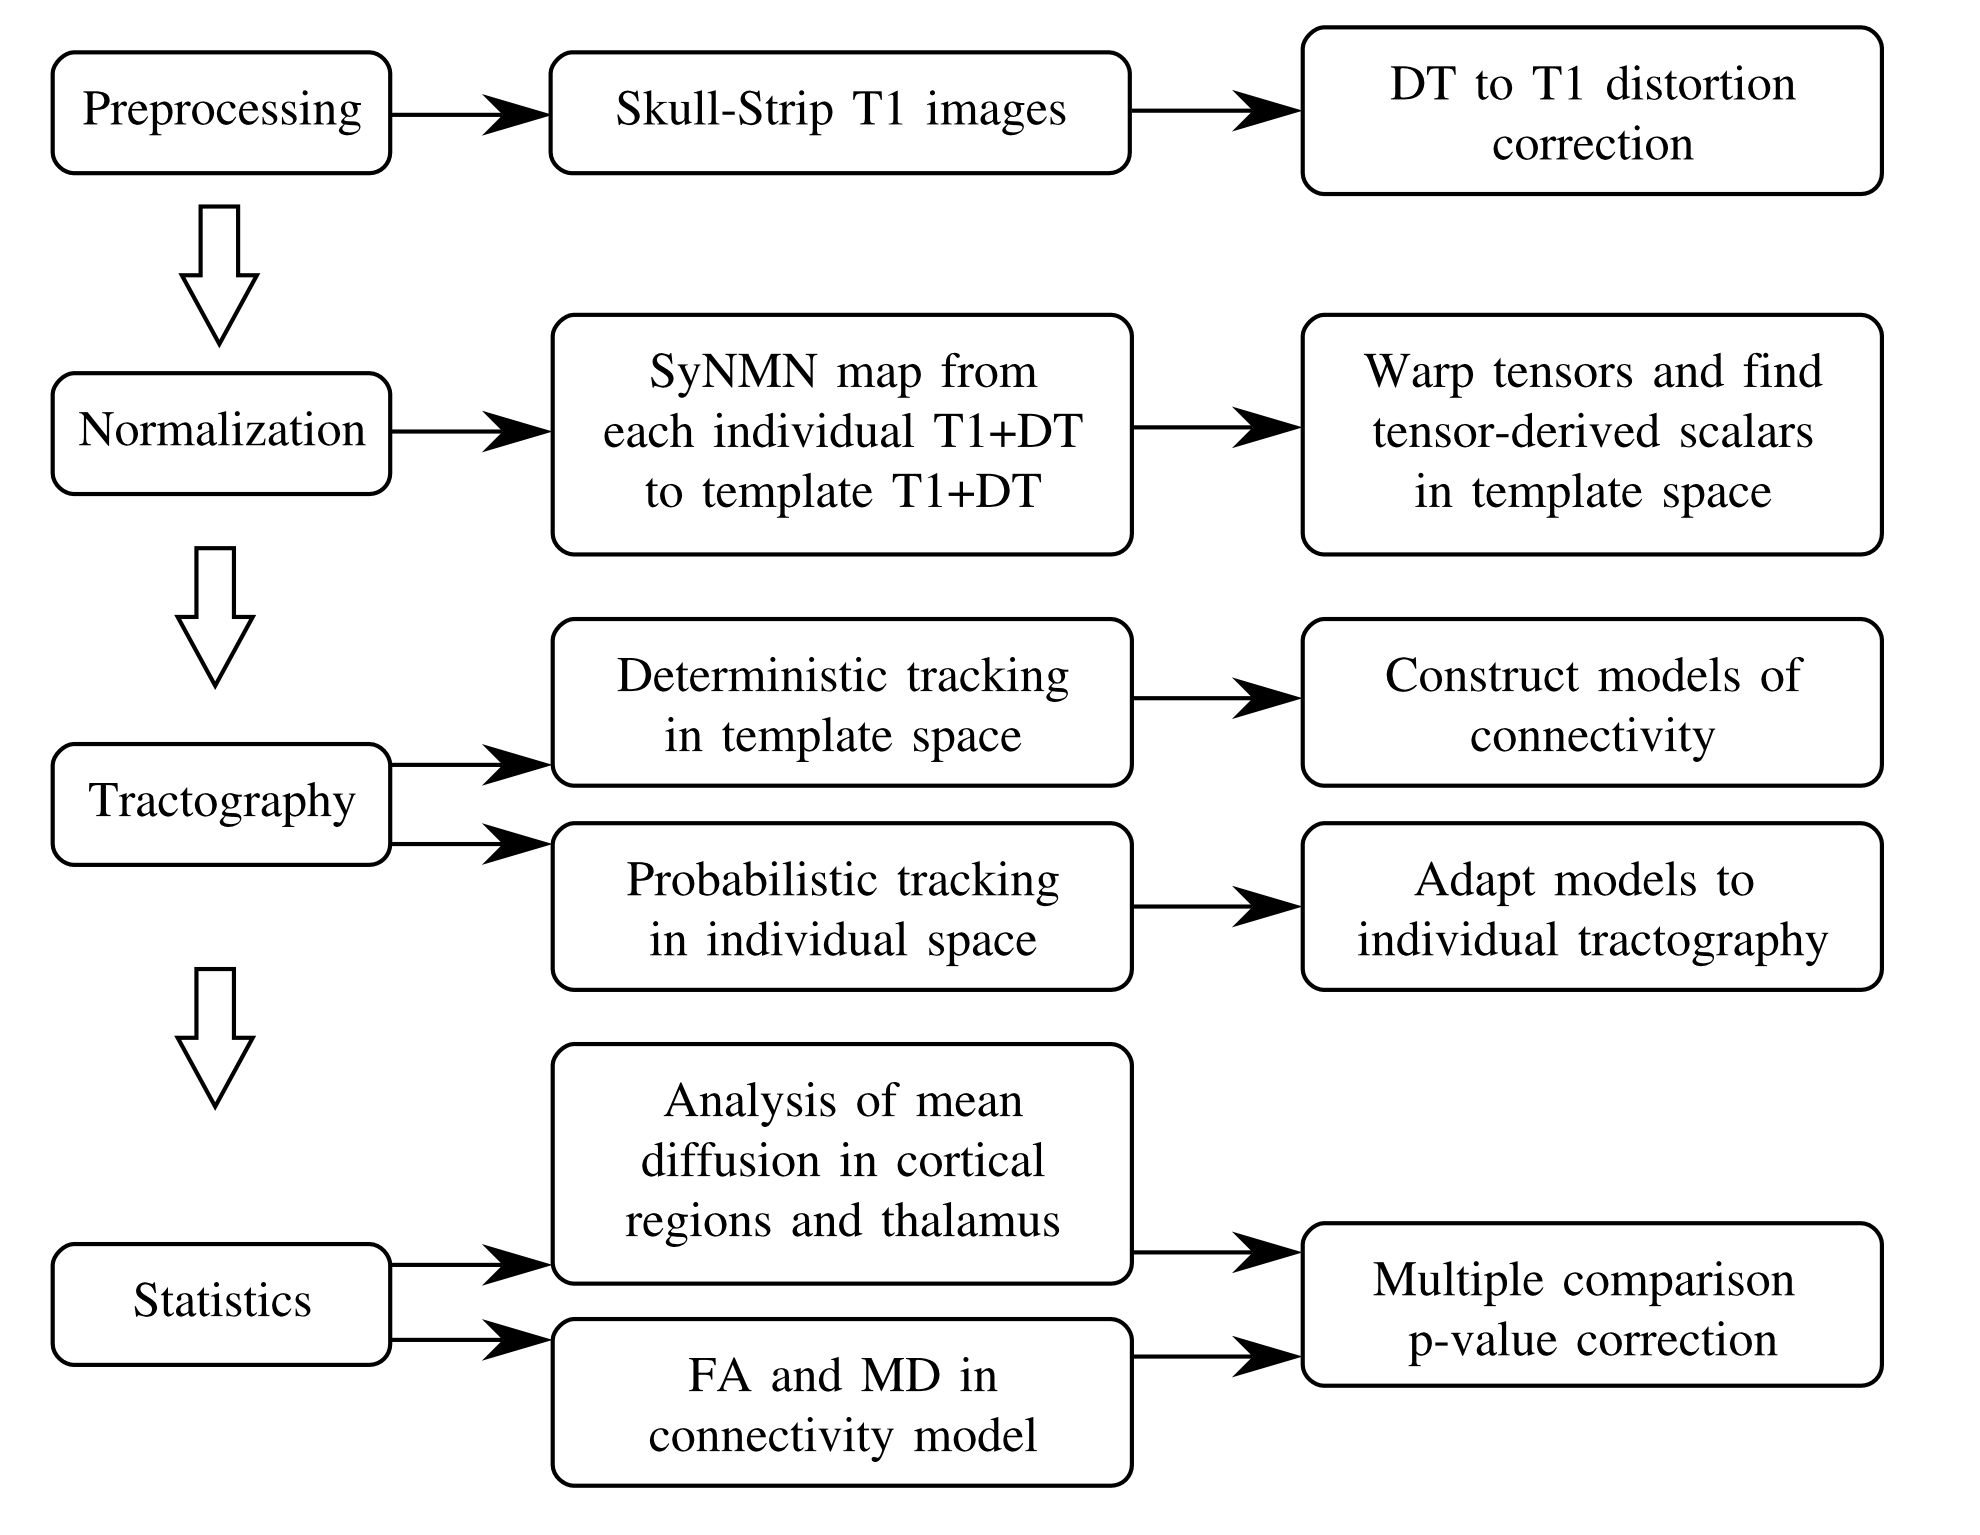
\includegraphics[width=0.9\linewidth]{figures/process.png}}
\caption{A overview of the steps required in the processing for
the population analysis of structure and connectivity.}
\label{fig:process}
\end{figure*}

\subsection{Cohort and Image Dataset}
The data was collected as part of a larger study investigating the neural correlates of attention deficits and treatment responses of
various psychoactive drugs in the survivors of TBI.  Our cohort included 10 individuals with TBI and 8 healthy controls. The 10 subjects with TBI included 6 men and 4 women aged between 21 and 59 years (mean age = 35.0, SD = 12.1) with a mean education of 13.3 years (SD = 1.7).  Control participants included 5 men and 3 women aged between 23 and 46 years (mean age = 36.2, SD = 8.8) with a mean education of 14.5 years (SD = 2.0).  The two groups did not differ significantly in terms of age, gender, ethnicity, handedness or years of education (tested with t-test or Fisher's exact test, as appropriate).

\subsubsection{Imaging parameters}
DT images were collected with a single-shot, spin-echo, diffusion-weighted echo-planar imaging (EPI) sequence and a GRAPPA parallel imaging acquisition.  The diffusion sampling scheme consisted of one image without diffusion gradients (b=0s/mm$^2$), followed by 30
non-collinear and non-coplanar diffusion encoding directions isotropically distributed in space (b=1000s / mm$^2$).  Additional imaging parameters were: TR=7300ms, TE=91ms, number of averages=1, and 1.875 mm$^2$ in-plane and 2mm out-of-plane resolution. High resolution T1-weighted anatomic images were obtained using 3D MPRAGE imaging sequence and the following acquisition parameters: TR = 1620 ms, TI = 950 ms, TE = 3 ms, flip angle = 15 degrees, 160 contiguous slices of 1.0 mm thickness, FOV = 192 $\times$ 256 mm$^2$, matrix = 192 $\times$ 256, 1NEX with a scan time of 6 min. The resulting voxel size was 1 mm$^3$.  All T1 images were skull-stripped by using symmetric normalization (SyN)~\cite{Avants2008} to map a brain mask from a template to each individual image.

\subsection{Normalization}
First an intra-subject, small deformation registration is performed with SyN, a univariate version of SyNMN, between each subject's T1 and FA images in order to correct for potential misalignment and distortion. The use of symmetric normalization techniques is particularly useful when working with both images and fiber tractography.  Image data is typically warped ``backward'' while point-based objects such as fibers are more easily warped ``forward'' using the inverse transform. Utilizing a method that inherently provides this symmetric mapping eliminates the need for {\em ad hoc} approaches for guaranteeing the invertibility of the transforms.
The normalization provided by SyNMN minimizes an energy function consisting of an image similarity term, $D_{sim}$, and a transformation metric distance term, $D_{shape}$, within the space of diffeomorphisms. This produces a series of maps, $\phi(x,t)$, that smoothly deform image $I$ into the space of image $J$ and, at the end point, $\phi(x,1.0)$, minimizes the following energy,

\begin{equation}
D_{shape}^2(\phi(x,0),\phi(x,1)) + D_{sim}(\phi(x,1),I,J)
\end {equation}

In order to examine both T1 and DT simultaneously, $D_{sim}$ is the weighted sum of two terms:
\begin{eqnarray}
D_{sim}(I,J,\phi) =& \omega_1(x)MI(I_{T1}(\phi_1),J_{T1}(\phi_2)) + \nonumber \\ &  \omega_2(x)\Vert(I_{DT}(\phi_1) - J_{DT}(\phi_2))\Vert_{DV}^2
\end{eqnarray}
where $MI$ is the mutual information and $\Vert(D_1 - D_2))\Vert_{DV}$ is the {\em deviatoric} Euclidean distance between two diffusion tensors~\cite{Alexander99}. Spatially varying weights are chosen to emphasize the tensor data in areas where the FA is high and prioritize the T1 data elsewhere. Additionally, it is desired that the weighting function be smooth. The first term of the weighting is given as $\omega_1 = G_{\sigma} \star (1.0 - FA(x))$ where $FA(x)$ is the 0.25 thresholded FA image and $G_{\sigma}$ is a Gaussian smoothing kernel operating on the weight function. The weights are constrained to sum to one so $\omega_2 = 1.0 - \omega_1$. The gradients of these terms are used to determine a mapping between any individual and a template using a standard multi-resolution gradient descent strategy. At each iteration, the DTI components are reoriented using the preservation of principal direction formulation~\cite{Alexander01}. Figure \ref{fig:atlas} illustrates the template provided by this technique. To examine the structural integrity of the cortical regions and thalamus, MD is examined at each point with a Student's t-test. We only consider results with an FDR-corrected p-value $<$ 0.02 and with a cluster size of at least 15 voxels.

\begin{figure}
\center{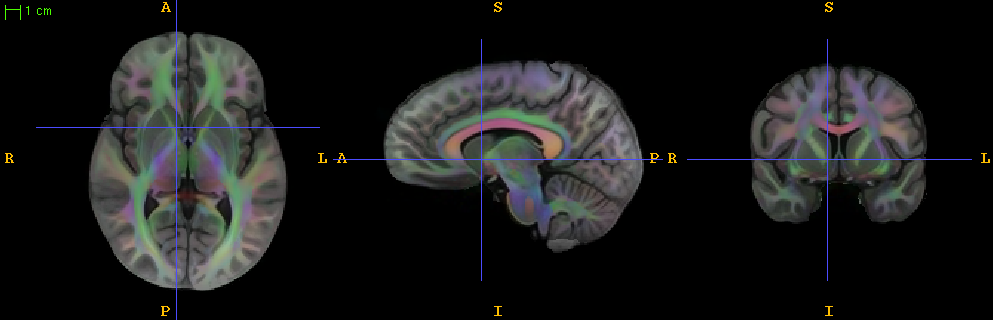
\includegraphics[width=1.0\linewidth]{figures/young_atlas_triplanar.png}}
\caption{Triplanar view of the combined T1 and DTI template provided by SyNMN. The directionally-encoded color map obtained from the principal direction of diffusion in the DTI data provides an overlay to the T1 data.}
\label{fig:atlas}
\end{figure}

\subsection{Connectivity Model}
In order to exploit both the tissue interface information provided by T1 data and the tissue architectural information provided by DTI, a normalization technique known as symmetric normalization of multivariate neuroanatomy (SyNMN) was used to create a population-specific template~\cite{Avants2007}. The use of a multivariate template is particularly useful when examining both gray and white matter properties. The T1 component of the template allows for the accurate identification of BA's as well as the thalamus. The DTI component provided the white matter orientation information that is essential to elucidating the connective pathways between structures. 

Recently, a number of studies have examined methods for using cortical atlases to label DTI generated fiber tracts according to their corresponding cortical regions. This concept has been used to develop connectivity based segmentations of structures such as the thalamus~\cite{Behrens03} and, more extensively, the corpus callosum~\cite{Styner05,Huang05,Hofer06}. Here a similar approach was used to label fibers but with the goal of developing a model of thalamo-cortical connectivity in the prefrontal lobe. To provide a framework for labeling fiber tracts by their associated cortical regions, the Brodmann area (BA) labels provided with the MNI atlas included as part the MRIcro package~\cite{mricro} were transformed into the atlas space by using SyN on the T1 component of the atlas. The FAST image segmentation package~\cite{Zhang01} was used to segment the T1 component of the template. All labeled voxels that were more than 5mm distant from the outer boundary of the gray-matter were excluded. An expert-knowledge guided manual segmentation of the thalamus was performed in the template using both T1 and DTI data. 
 
The DTI component of the template provided a smooth tensor field that was well suited for identifying white matter tracts that are often difficult to track reliably in subject data due to noise. Large bundles of fibers were found for each thalamus to BA connection and were used to determine a model tract for each connection. Whole-brain deterministic tractography was performed using the Camino Toolkit~\cite{Cook06} where all voxels with an FA greater than 0.15 were used as seed points. A constant step size of 0.3 mm was used along with linear interpolation of the principal direction of diffusion vector field. Fibers were terminated when they entered a voxel with FA less than 0.15 or when local curvature of a fiber exceeded 45 degrees. The segmentation of the thalamus and cortical regions allowed for the extraction of fibers connecting these regions. For the purpose of this study, we limited the fibers to those in the anterior thalamus radiata (ATR) which connect the thalamus to BA's 9,10, and 11.

DTI tractography methods are known to produce a number of false-positive pathways. To exclude these, each fiber bundle was filtered to remove fibers of excessive length as well as fibers whose cortical end points were distant from the average end point location. The remaining fibers were then smoothed with BSplines~\cite{Tustison06} and a curve matching algorithm examined local curvature properties~\cite{Avants2003b} to identify corresponding locations on each fiber. A BSpline was fit to the set of corresponding locations on all fibers to determine a final approximation of the white matter pathway. Finally, the curve matching algorithm was used to match the corresponding models in each hemisphere to ensure a consistent parameterization. The model is illustrated in figure \ref{fig:model}. 

%\begin{figure*}
%\center{\includegraphics[width=0.8\linewidth]{model.png}}
%\caption{Thalamo-cortical connectivity models for the prefrontal lobe are created using deterministic tractograpy in a subject-specific atlas. BA's 9 (blue), 10 (purple) and 11 (pink) are used to label the streamlines that connect each region to the thalamus.  Model connections are visualized as tubes with colors corresponding to their cortical regions. The streamlines used to determine the model connections are shown with complementary colors}
%\label{fig:model}
%\end{figure*}

\begin{figure*}
\begin{center}
$\begin{array}{c}
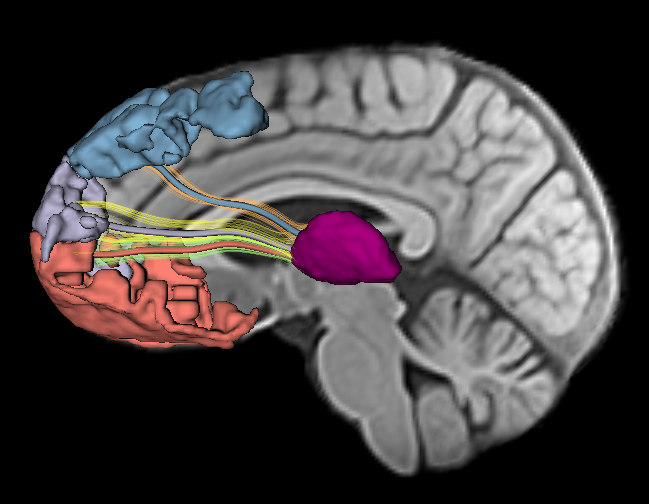
\includegraphics[width=0.75\linewidth]{figures/model1.png} \\
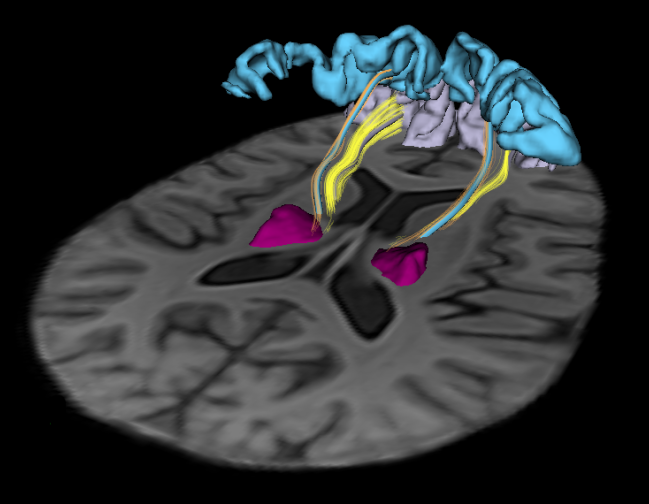
\includegraphics[width=0.75\linewidth]{figures/model2.png}
\end{array}$
\caption{Thalamo-cortical connectivity models for the prefrontal lobe are created using deterministic tractography in a subject-specific atlas. BA's 9 (blue), 10 (purple) and 11 (pink) are used to label the streamlines that connect each region to the thalamus. Model connections are visualized as tubes with colors corresponding to their cortical regions. The streamlines used to determine the model connections are shown with complementary colors.}
\label{fig:model}
\end{center}
\end{figure*}

\subsection{Subject Specific Connectivity Models}
Because the normalization method used does not explicitly match based upon the connectivity between distant structures in the brain it was necessary to identify these pathway in each individuals' DTI data in order to evaluate the usefulness of the template generated model tracts. We warped the model tracts into subject space and used them to search for similar tracts in the probabilistic tractography. This provided a common frame-of-reference for inter-subject comparison while still relying on the tractography obtained from each individual. The transform obtained in the normalization process was used to warp the segmented thalamus and labeled cortical regions in to each individual's native DTI space. All points in the thalamus were used as seed points for wild bootstrapping probabilistic tractography using the Gaussian model of diffusion~\cite{Jones06,Whitcher08}. From each seed point, 1000 fibers were tracked and those that hit labeled cortical regions were retained and labeled. 

Probabilistic tractography methods generate a very large number of tracks which can make processing cumbersome and interpretation difficult. The model tracts were warped into the subject space and served as a framework for determining subject specific model tracts from the probabilistic tractography results. Within each labeled bundle of fibers the mean point-to-point distance between the model tract and each probabilistic tract was used to initially prune the bundle to include the N-closest fibers (N=200). Many of the probabilistic tracts only contained partial segments that were within the specific pathway being examined. This makes the whole-fiber curve matching technique used in the creation of the models unsuitable for use on probabilistic fiber tracts. Instead a point-by-point approach was taken to focus on local properties of the fiber tracts. At each point, $x_m$, in the model the closest point, $x_i$ on each of the N-closest fibers was found, and a weighting was calculated via:
\begin{equation}
\omega_i = e^{\frac{-|x_m - x_i|}{\sigma}}
\end{equation}
The k-highest weights are selected and normalized to sum to one. Here we used $k=40$ and $\sigma=2.0$. A BSpline was used to fit a curve to these weighted points. Additionally, the points and their associated weights were used to calculate a log-Euclidean average tensor at each point~\cite{Arsigny06}. These average tensors were then used to calculate tensor-derived scalars such as FA and MD. Figure \ref{fig:fitting} provides and illustration of the results of the subject specific fitting.

\begin{figure}
\center{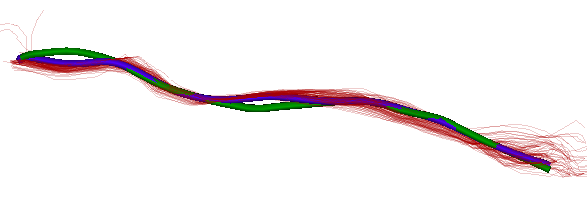
\includegraphics[width=0.75\linewidth]{figures/fitting.png}}
\caption{The connectivity model (green) was warped into the subject space via the transform provided by SyMNM. The results of probabilistic tractography (red) in the individual were then used to adapt to the model to the subject resulting in a model (blue) that more closely represented the subject's anatomy.}
\label{fig:fitting}
\end{figure}

The model tracts were defined in a smooth template space which could reduce their utility in identifying focal differences. In order to evaluate the extent to which this is true, we evaluated a population using both subject-space models and the original model tracts. To do this, we used the model tracts, the template space tractography, and each subject's warped tensor data to determine an average tensor at each point in the tract. When determining the k-closest points, the results of the curve matching obtained in the creation of the model were used to limit the search to the set of corresponding points from each fiber. Otherwise, the process was the same as that taken when using the subject specific tractography. Figure \ref{fig:exconnections} provides an illustration of this technique in both subject-specific and template space. By examining FA and MD along fibers in both the template models and the the subject space models we hoped to gain further insight into each method's ability to identify differences in populations.

\begin{figure*}
\begin{center}
$\begin{array}{ccc}
\textrm{Control} & & \textrm{TBI} \\
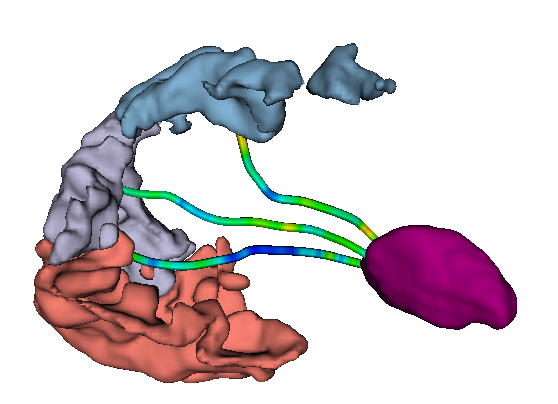
\includegraphics[width=0.4\linewidth]{figures/dc02full.png} & &
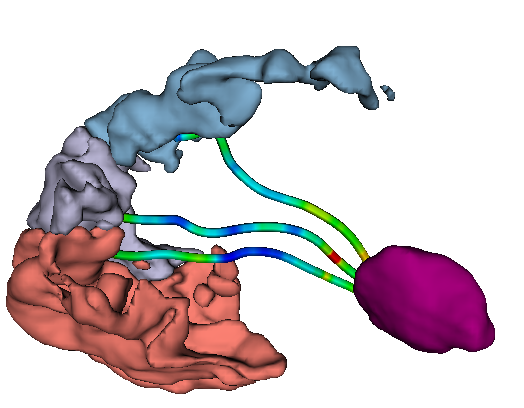
\includegraphics[width=0.4\linewidth]{figures/dp09full.png} \\
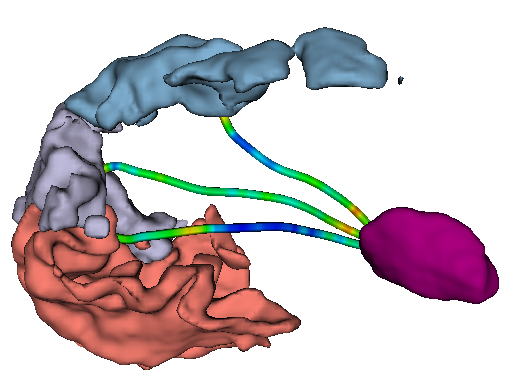
\includegraphics[width=0.4\linewidth]{figures/dc05full.png} & 
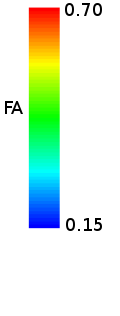
\includegraphics[width=0.1\linewidth]{figures/colorbar.png}&
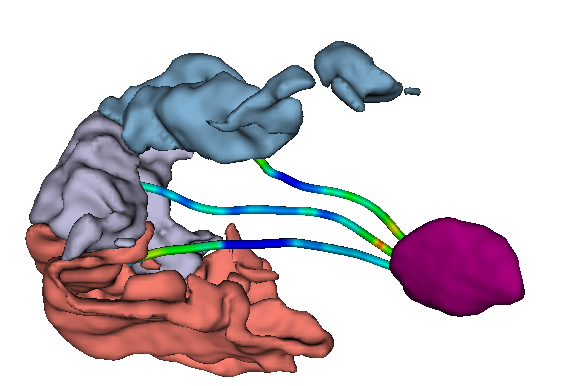
\includegraphics[width=0.4\linewidth]{figures/dp07full.png} \\
 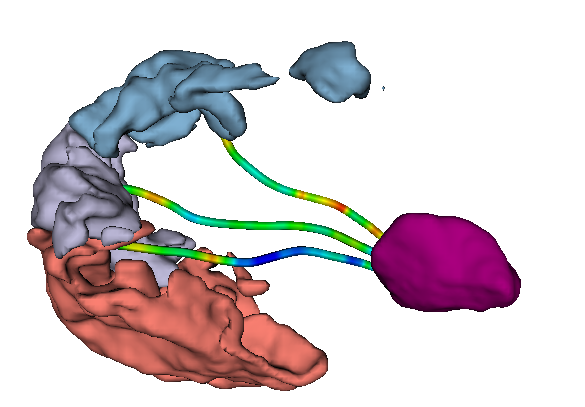
\includegraphics[width=0.4\linewidth]{figures/dc04full.png} & &
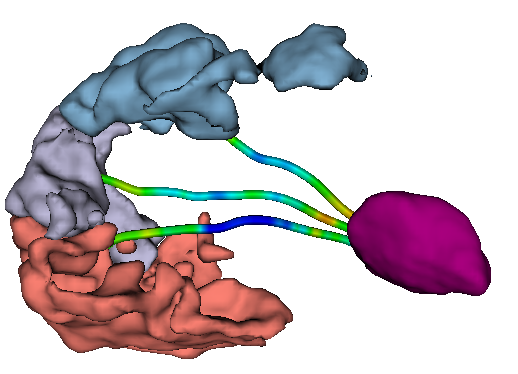
\includegraphics[width=0.4\linewidth]{figures/dp08full.png} \\
\end{array}$
\caption{Subject specific connectivity models for connectivity between thalamus (purple) and BA 9(light blue), 10 (light purple) and BA 11 (pink) are illustrated for three controls (left) and three subjects (right). The connectivity models are colored by average fractional anisotropy.}
\label{fig:exconnections}
\end{center}
\end{figure*}

\section{Results} 
To examine the structural integrity of the cortical regions and thalamus, MD was examined at each point with a Student's t-test. We only considered results with an FDR-corrected p-value $<$ 0.02 and with a cluster size of at least 15 voxels. Compared to controls (N=8), TBI survivors (N=10) showed increased MD in the mediodorsal nucleus of the thalamus~\ref{fig:volstats}. Both the subject-specific and template models were used to examine FA and MD along each connection using a Student's t-test at each point. We only considered results with an FDR corrected p-value $<$ 0.02 and with a 1-D cluster size of at least 5. Figure \ref{fig:connstats} shows the FA differences in the connectivity models of the ATR between control and individuals with TBI as determined by subject-specific connectivity models as well as template space models. In both subject-specific and template space analysis, TBI survivors showed reduced FA near the midpoint of the connection between the thalamus and BA 10 in the left hemisphere. The cluster was located at approximately the same location in each model and is slightly larger in the template space model than in the subject-specific model. The cluster in template space had a maximum t-value of 4.60 while the cluster in the subject-specific analysis had a maximum t-value of 5.26.

\begin{figure}
\begin{center}
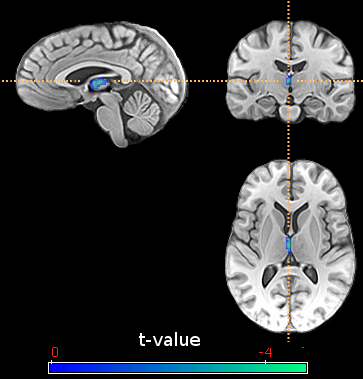
\includegraphics[width=1.0\linewidth]{sigmd.png}
\caption{Mean diffusion is examined in the cortical regions and thalamus. Results with an FDR-corrected p-value $<$ 0.02 and a cluster size of 15 voxels or greater are visualized.}
\label{fig:volstats}
\end{center}
\end{figure}

\begin{figure*}
\begin{center}
\begin{tabular}{ccc}
\multicolumn{3}{c}{Location of fractional anisotropy reduction in TBI} \\
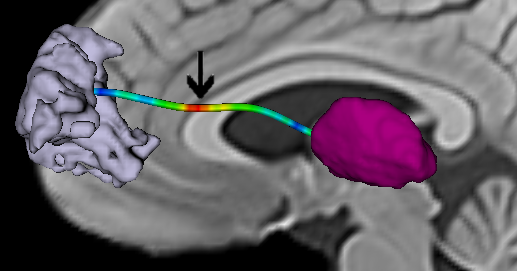
\includegraphics[width=0.42\linewidth]{figures/subject_tstat.png} &
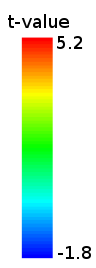
\includegraphics[width=0.08\linewidth]{figures/tcolorbar.png}&
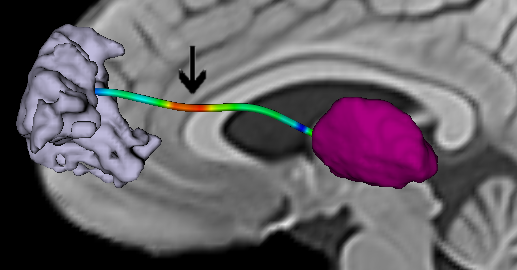
\includegraphics[width=0.42\linewidth]{figures/template_tstat.png} \\
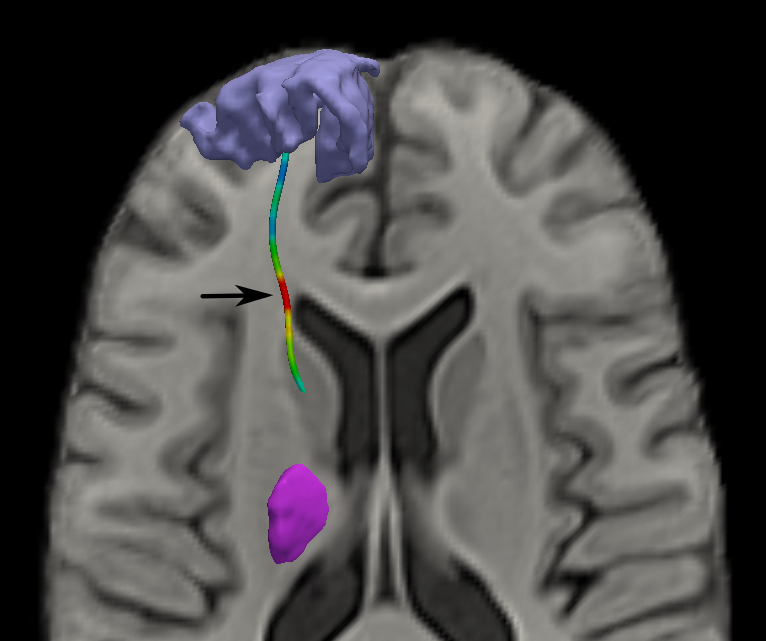
\includegraphics[width=0.42\linewidth]{figures/tbi_subject_axial.png} & &
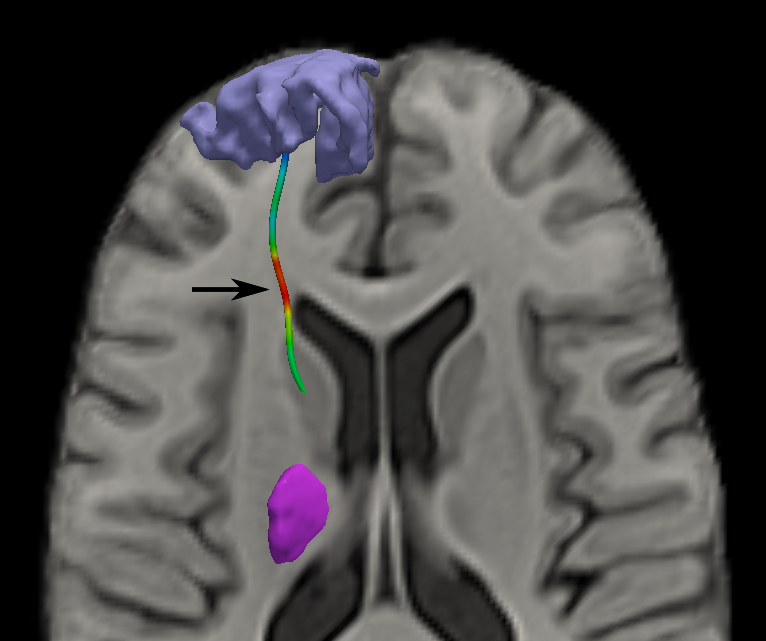
\includegraphics[width=0.42\linewidth]{figures/tbi_template_axial.png} \\
\textrm{Subject space} & & \textrm{Template space} \\
\end{tabular}
\caption{Students t-test results after FDR correction at p$<$0.02 indicated that the left hemisphere connection between thalamus and Brodmann area 10 is affected by TBI. Arrows indicate regions where TBI survivors showed reduced FA compared to controls in both subject space (left) and template space (right) analysis. Sagittal and axial slices from the T1 component of the template are shown for anatomical reference.}
\label{fig:connstats}
\end{center}
\end{figure*}

\section{Discussion}
This study demonstrated that multivariate image registration techniques may be combined with diffusion tensor tractography to create a system-based model for delineating both structural and connective differences in TBI. Localized differences in MD were found in the mediodorsal nucleus of the thalamus. An examination of the white matter fibers that connect this region of the thalamus to the prefrontal cortex revealed significant clusters indicating reduced FA in TBI. The use of a connectivity model that adapts to individual subject data produced similar results but with a more focal cluster and a higher peak t-value.

Our findings in this subset of the limbic system support previous in-vivo neuropathologic studies~\cite{Graham2005,Maxwell2006} as well as in-vivo volumetric studies which have identified significant damage to the mediodorsal thalamus resulting from head injury~\cite{Kim2008}. The difference in MD in the thalamus suggested a difference in the structural integrity of the tissue which is complementary to previous findings of volume reduction in that area\cite{Kim2008}. The mediodorsal thalamus is known to be heavily connected to the prefrontal cortex~\cite{Goldman85}, a region believed to play a vital role in the mediation of executive function and motivation. In the thalamo-cortical connections, reduced FA and increased MD were detected, both of which suggested a degradation of cellular integrity in the white matter and supported the concept of using DTI as a basis for elucidating information regarding diffuse axonal injury~\cite{Huisman04}. Our results provided a neuroanatomical interpretation for the observed psychological impairments in TBI survivors, such as lowered motivation~\cite{Kraus2007,O'Sullivan2004} and frequency of depression~\cite{Drevets2000,Chen2008}.  

It should be noted however that caution must be taken when interpreting differences found in tensor-derived scalars. In the case of TBI however, it seems likely that that increases in MD and decreases in FA result from underlying tissue damage. These findings supported the belief that damage to structures such as the thalamus results in subsequent damage to the white matter tracts associated with that structure. Additionally, while these measures may be used to infer damage to the underlying tissue they do not directly provide a measure of connectivity. While of great interest to many, the ability to use DTI to obtain physiologically relevant measures of connectivity between distant structures is still an unresolved issue and is the subject of ongoing research.

The results provided by the subject-specific analysis were similar to that of the template based method, but suggested a more focal difference. As the template provides a smoother representation, this in an expected result.  However, further study is required to fully understand potential benefits and short-comings of the subject-specific methods. The use of template streamlines in the creation of a connectivity model is a natural extension to DTI tractography, however it is important to consider alternative representations. Recent work has used medial surfaces to parameterize ``sheet-like'' fiber tracts~\cite{Yushkevich08}. This type of representation could provide a more anatomically relevant method for representing the fibers associated with BA's 10 and 11. Other shortcoming in the study include small population size, wide range of ages and variable mechanism of injury. Variation in time between injury and imaging is also an important issue.

Here probabilistic tractography in the individuals was used to adapt the general models to each subject's anatomy. Due to the nature of these probabilistic methods, this required a great deal of processing to identify the appropriate trajectories. Here we relied upon tractography in the individual space, however including information directly from each individual's underlying tensor field is a potential method for enhancing the subject fitting. Expanding the model to include additional connections would provide additional insight into the complex effects of TBI. Previous tractography studies of the thalamus have shown the ability to track fibers emanating from the posterior portion of the thalamus that connect to BA 11. This is particularly relevant as that cortical region is involved in many processes related to symptoms often found in TBI survivors.

In conclusion, traumatic brain injury leads to complex effects in the cortex, deep gray matter structures and the connections between them. We used SyNMN, a cutting-edge technique for multivariate image registration, to create a template space in which we define a connectivity model. The connectivity model was then used as a prior for identifying analogous white matter connections in individual tractography data. Additionally, this model provided a common frame-of-reference in which to compare metrics along the fiber pathways. We demonstrated that adapting the template model to individual subject data impacts the statistical significance in a study of a patient population. In particular we found evidence of injury in fiber pathways associated with thalamo-cortical connections. 


\chapter{Structural and functional connectivity influence decision-making in communication}
\label{chap_homo}

The brain's language network has been the focus of much research relating function to underlying structure, although assessments of white matter connectivity within the language network have been rare. In this study, we examine measures from event-related functional MRI and integrate these with diffusion tensor imaging tractography and cognitive performance in 10 healthy right-handed control subjects. A communication-based decision-making task was used to identify a functional network via fMRI. Diffusion tensor tractography was used to identify the fiber tracts that provide the biological network of connections between the nodes of the functional network. Functional connectivity between regions was measured by correlating region averaged fMRI time signals and structural connectivity was measured with the average fractional anisotropy in the fiber tracts that connect the cortical regions. Stepwise multiple linear regression analysis was then used to identify the functional and structural connections that most significantly regulate cognitive performance. Both structural and functional analyses suggest that performance depends on the integration of language and decision-making subnetworks during task performance, and regression analyses suggests that measures of statistically-based functional connectivity are more sensitive than  structural connectivity at demonstrating integration within this large-scale network, but that the influence of structural connectivity is more distributed throughout the network.

%% main text
\section{Introduction}
\label{Intro}
The human brain is a system comprised of a vast number of neurons that provide great computational capacity via a complicated communication network consisting of both local circuits and long-range fiber pathways. The neurons of the cortical gray matter are responsible for processing information while the axons projecting from these neurons in the white matter provide the communication channels between the functionally and structurally segregated subregions of the cortex. The study of brain connectivity seeks to understand the interconnections, structural properties, and functional relationships of the elements of this system and is essential for further insight into the nature of complex cognitive processes supported by large-scale neural networks. In this study functional networks in the brain are examined using magnetic resonance imaging (MRI) to measure both structure and function. We hypothesize that cognitive performance will be more sensitive to the structural properties of the white matter that provides the biological network of connections than to the statistical measures of functional connectivity within the network. Tasks involving language processing and decision-making were used along with fMRI to identify the cortical regions utilized by then functional network and to allow assessment of functional connectivity between these anatomically distinct regions during performance of the tasks. Diffusion tensor imaging (DTI) was used to identify and examine the structural properties of the white matter fiber bundles that provide the communication channels between the functional regions. The network-wide measures of functional and structural connectivity were then independently used to examine their influence upon a behavioral measure of performance on the functional tasks.

\subsection{Structural Connectivity}
The set of all biological connections in the brain is known as the human connectome and provides a basis for the examination of structural connectivity~\cite{Sporns2005}. Understanding the structural connective patterns in the brain is essential to gaining further insight into the complex functional interactions that are required for complex behavior. In addition to identifying these biological connections, measuring their quality or integrity is critical to understanding the relationship between structure and function and how these together modulate behavior.  Neuroimaging techniques provide an in-vivo, macro-scale basis for a variety of methods that identify these biological connections and/or examine the structural properties of the tissues that comprise them. Studies of structural connectivity typically focus upon examining the myelinated neurons of the white matter that connect gray matter regions. In diseases that cause demyelination, anatomical images (e.g. T1- or T2-weighted images) may be used to identify white matter lesions that disrupt connectivity~\cite{Loevblad2010}. Measures of structural connectivity may also be inferred by measuring the size of white matter structures, an approach that has been used extensively to study the mid-sagittal cross-section of the corpus callosum~\cite{Witelson1989,Colcombe2005a,Gunning-Dixon2000}. 

\subsection{DTI and Structure}
Recently, the use of diffusion tensor imaging (DTI) has received a great deal of interest as a method for examining structural connectivity. DTI provides information about the orientation and micro-architecture of white matter~\cite{Basser1996}. This arises from the fact that myelin provides a barrier to the diffusion of water resulting in diffusion anisotropy where the diffusion of water is much greater along the direction of the axons than across. The orientation information provides the basis for fiber tractography methods that identify physical connections in the form of estimated white matter trajectories ~\cite{Basser2000,Mori1999a}. Measures of diffusion anisotropy, such as fractional anisotropy (FA), allow for quantitative measures of white matter integrity.  While confounded by issues such as (a) limited spatial resolution, (b) generation of false-positive connections, and (c) inability to distinguish between multiple fibers traveling in different directions within a single voxel, DTI based methods have proven useful in the examination of large, well-defined white matter fiber tracts such as the commisural fibers of the corpus callosum, the projection fibers of the thalamo-cortical network, and the association fibers of the language network. Identifying the cortical regions to which these fiber bundles extend provides the ability to examine the topography of specific white matter pathways~\cite{Behrens2003} as well as the properties of the underlying tissue. 

Following the classical anatomical teachings of connections and behavioral neurology ~\cite{Geschwind1965b,Geschwind1970}, DTI studies of living humans have demonstrated asymmetries in the left and right hemispheres of neurologically intact adults that reflect the known lateralization of language~\cite{Catani2008,Glasser2008}. Attempts have been made to relate this anatomic asymmetry to the language network. For example, an examination of the fiber tracts of the language network and demonstrated that inter-hemispheric symmetry in the arcuate fasciculus is associated with enhanced ability to remember words using semantic association ~\cite{Catani2007}. The relevance of structural connectivity to behavior was demonstrated more directly in work that found that increased FA in the white matter associated with Broca's area was higher in subjects with better grammar learning~\cite{Floel2009}. Further evidence for the behavioral relevance of FA was provided in the first study to provide evidence for white matter changes resulting from training in healthy human brain~\cite{Scholz2009}. Localized increases in FA were detected in the white matter of the intraparietal sulcus following training of a complex visuo-motor task (juggling) ~\cite{Scholz2009}. 

\subsection{Functional integration and connectivity}
Blood oxygenation level-dependent (BOLD) fMRI provides a method for measuring activation in the brain. By contrasting the activation levels associated with different experimental conditions, it is possible to identify cortical areas that are associated with specific tasks such as language processing~\cite{Frost1999,Bookheimer2002} and decision-making~\cite{Sanfey2003,McCabe2001}. To perform complex tasks, it is necessary for several anatomically distinct but functionally co-activated regions to work together and form networks under a concept known as functional integration. One way to study this integration is to examine the statistical covariance of BOLD activation in several cortical regions activated during task performance across a population~\cite{Horwitz1990,McIntosh1994}. Functional connectivity uses one of several statistical paradigms to identify coordinated activity in spatially distinct units in an individual's brain~\cite{Rykhlevskaia2008}. 

In this study, we examine the relative informativeness of functional connectivity compared to biological connectivity defined by DTI. To examine biological networks based on white matter tracts defined by DTI compared to functional connectivity defined statistically, we assessed a BOLD fMRI data set collected during an fMRI language activation study of homonyms~\cite{McMillan2010}. Briefly, this study asked subjects to make decisions about the use of a homonym or a non-homonymous synonym in a sentence. The authors hypothesized that participants would prefer to use the dominant meaning of a homonym in a context-appropriate sentence (e.g.\ ``pen" to refer to a writing implement), but would prefer to use a synonym instead of the subordinate meaning (e.g.\ ``cage" instead of ``pen" to refer to an animal enclosure). The authors demonstrated different fMRI activation patterns for each condition. A language network was recruited in the left hemisphere during stimuli with the dominant meaning, but a decision-making network was recruited additionally during subordinate stimuli. We examine the interactions between language and decision-making subnetworks using statistically-based functional connectivity and DTI-based assessments of white matter projections between activated language and decision-making regions.

\subsection{Relationship of Structure and Function}
Previous studies have attempted to combine BOLD fMRI and DTI measures in tracts between activation brain regions.
The first study to combine fMRI and DTI examined a single patient's recovery from a traumatic brain injury~\cite{Werring1998a}, and employed a converging evidence approach that relied upon qualitative analysis and formed a basis for many additional studies~\cite{Werring1999b,Jang2005,Klein2007,Munakata2006,Shinoura2006,Koch2002a}. A variety of quantitative approaches to combined analysis of DTI and BOLD fMRI have been developed. In one approach, voxelwise correlations were performed between functional and structural connectivity maps ~\cite{Olesen2003,Thomas2009}. These methods were not particularly informative because they did not heed the anatomical tracts projecting between activate regions. More recently, fMRI has been combined with DTI tractography by using functionally activated regions as seeds for tractography~\cite{Toosy2004,Powell2006,Upadhyay2007,Boorman2007,Jenkins2010}. Unless carefully constrained, this may result in the inclusion of white matter that, despite connecting to a cortical region of interest, is not part of the functional subnetwork being examined. Here we combined information from structural and functional data to restrict the analysis to fiber bundles that provide a direct biological connection between any two functional regions of interest. 

\subsection{Incorporation of Behavioral Data}
Finally, using behavioral data collected during the fMRI study as the dependent variable, we examine the relative effectiveness of statistically-based functional networks and DTI-based white matter networks to explain performance. Some previous work has related DTI and fMRI to performance. For example, Baird, et al.\ \cite{Baird2005} used reaction times and fMRI to localize cortical activity for short and long reaction times. Regression analysis using BOLD values in the activated regions as independent variables was then used to show that short reactions times were associated with FA in the splenium of the corpus callosum while long reaction times were associated with FA in the genu of the corpus callosum~\cite{Baird2005}. A study by Madden et al.\ \cite{Madden2007} combined DTI and fMRI to study the effect of aging on visual response time. Activation in the frontal and parietal cortical regions was shown to be greater for older adults, but while an age-related FA decrease was found in older adults, it did not specifically mediate the age-related changes in activation~\cite{Madden2007}. An examination of executive cognition found white matter development and age-related changes in fMRI to be directly associated with cognitive performance~\cite{Stevens2009}. Recent work by Propper et al.\ \cite{Propper2010} examining handedness and it's influence upon functional language lateralization and structure in the arcuate fasciculus suggested that degree of handedness may be an important to consider in studies of neuroanatomical asymmetries.  We hypothesize that both functional and structural connectivity may predict cognitive performance and that a stepwise multiple linear regression analysis of cognitive performance will reveal the components of the network that most influence performance. 

\section{Methods}

\subsection{Subjects}
Ten subjects (6 female) ranging in age from 19 to 32 years (mean age of 23.5 years) had both functional and diffusion tensor images. All subjects were healthy young adults participating in the study for monetary payment. All participants were native English speakers, right-handed and in good health with no history of neurological difficulty. Informed consent was obtained from all participants according to a protocol approved by the University of Pennsylvania Institutional Review Board. 

\subsection{Subnetworks in the brain} 
We investigate a hypothesis proposed by McMillan et al.\ ~\cite{McMillan2010} that suggests language processing is supported by the interaction of two cortical subnetworks, one for language and one for decision-making. This study specifically focused on the strategic process of minimizing ambiguity during language production, defined as an individuals' use of an unambiguous word (e.g.\ ``cage") instead of a semantically ambiguous word (e.g.\ ``pen") to make the meaning of an utterance more clear. A forced choice paradigm was used in which subjects were instructed to make the choice that resulted in the most clear sentence meaning (e.g.\ reduced ambiguity). 20 homonyms were identified that had a strong bias toward one of the possible meanings. The more frequent meaning (e.g.\ ``pen" is used to refer to a writing implement) is referred to as dominant while the less frequent meaning (e.g.\ ``pen" is used to refer to an animal cage) is referred to as subordinate. For each homonym, 3 context sentences were generated in which the final word was semantically related to the dominant meaning, subordinate meaning, or was semantically neutral in meaning. Additionally, a carrier sentence was generated for each homonym that consisted of a short phrase followed by a blank space. The same carrier sentence was used for dominant, subordinate, and neutral contexts for each homonym.  Lastly, a semantically related unambiguous alternative was generated. These sentences were used to create 60 experimental trials using each of the 20 homonyms in each of the contexts (dominant, subordinate, neutral). Example sentences for each condition are provided in table~\ref{sentences}~\cite{McMillan2010}. Participants were presented with a context sentence, a carrier sentence and choice between a homonym and an unambiguous alternative. To limit the participants' ability to reduce the task to homonym detection, 180 filler trials were used that followed the same format but did not include a homonym. Experimental and filler trials were randomly distributed into 5 fMRI runs of equal length. The frequency with which participants chose the unambiguous choice was recorded and used as the measure of cognitive performance.

\subsection{MRI Acquisition}
Scans were acquired on a Siemens 3.0T Trio scanner. T1-weighted structural images were acquired using an MPRAGE protocol ($TR = 1620 ms$, $TE = 3 ms$, flip angle of $15^{\circ}$, 1 mm slice thickness, $192 \times 256$ matrix, resolution = $0.9766 \times 0.9766 \times 1.0 mm$). BOLD fMRI images were acquired with fat saturation, 3 mm isotropic voxels, flip angle of $15^{\circ}$, $TR = 3 s$, $TEeff = 30 ms$ and a $64 \times 64$ matrix. DT-MRI images were acquired with 4 $b=0$ images and 30 directional diffusion weighted images (resolution = $1.875 \times 1.875 \times 2.0 mm$, $112 \times 112$ matrix, $b=1000 s/mm^2$). 

\subsection{fMRI analyses overview}
For the examination of function, the cortical regions identified by McMillan et al.\ were examined~\cite{McMillan2010}. All regions but one activated the left hemisphere. In order to limit our study to the left-hemisphere we use the left homologue to the right interior parietal region that was activated in the McMillan et al.\ study. While 18 subjects were studies by McMillan et al.\, we include only the 10 subjects for which DTI was also acquired in order to examine the relationship between function and structure. Processing of the fMRI data was performed using SPM5~\cite{SPM5}. For each subject, the functional data was motion-corrected, transformed into MNI space, spatially smoothed with a 8mm FWHM isotropic Gaussian kernel and interpolated to isotropic 2 mm voxels. A canonical hemodynamic response function was used to convolve the onset times of stimulus events for each condition. A general linear model approach was then used to calculate statistical parameter estimates for each subject. Each coordinate listed in table~\ref{PeakCoords} was used to define the center of spherical region of interest (ROI) with a 10mm radius. 

Statistically based connectivity was determined in the following manner. For each ROI in each subject, an average t-value was calculated for each context (i.e.\ dominant, neutral, subordinate). These region averaged activation values were used to examine the covariation of activation across the population via correlation analysis using Pearson's correlation coefficients. Specifically, activations corresponding to responses to each of the categories of stimuli were extracted from the fMRI time-course signal to create a time-signal with 20 time points for each context. For each ROI, the context-specific time-courses from all voxels within the ROI were used to determine an averaged time-signal for that region. These time-signals were then normalized to have a mean of 0.0 and a standard deviation of 1.0. To estimate intra-subject functional connectivity under each context, a Pearson's correlation coefficient was calculated for each region-to-region pair of interest within each subject. We limited the analysis to pairs of regions that have direct biological connections as our primary interest is in examining the relationship between structure and function and due to the limited size of the data set being examined.

\subsection{DTI analyses}
For the examination of structure, the cortical regions identified by McMillan et al.\ \cite{McMillan2010} were used to identify the white matter fiber bundles that define the biological connective network that provides communication between cortical regions. The white matter tracts of interest were identified in a diffusion tensor atlas and used to create geometric models. The models were then used to examine FA in each subject. Average FA values for each structure were calculated to provide an equidimensional framework for relating these structural measures to the functional connectivity measures that were calculated for the regions connected by each fiber tract. Specifically, we used an atlas-based methodology that provides a common anatomical frame-of-reference for inter-subject comparisons, an approach used in methods designed to identify focal white matter differences~\cite{Yushkevich2008,Goodlett2009a,Jones2002,Xu2003,Smith2006}. Fiber template were used to create arc-length parameterizations of diffusion properties due to their ability to examine whole-tract properties of white matter pathways~\cite{Jones2005,Corouge2006,Maddah2008d,Lin2006,ODonnell2009,Davis2009,Goodlett2009a,Batchelor2006}. Defining these fiber templates in the atlas space avoids the time-consuming and error-prone process of defining anatomically equivalent ROIs in each subject~\cite{Gilmore2007}. Moreover, the improved SNR provided by a population atlas provides an appropriate space for identifying fiber bundle geometry and minimizes false-positive errors~\cite{Goodlett2009a}. 

A multivariate atlas was created from a data set consisting of 30 healthy young adults for whom both high resolution T1 images and DTI were acquired. The 10 subjects from the functional study that also had DTI data were all included in this atlas-building data set. The set of all subjects' high resolution T1 weighted images were used to create an unbiased, shape averaged atlas using Symmetric Normalization as implemented in Advanced Normalization Tools (ANTS)~\cite{ANTS}. This was accomplished through the use of a multi-resolution, non-rigid registration algorithm to optimize a cross correlation metric under the constraints of a diffeomorphic transformation model~\cite{Avants2006}. The Brain Extraction Tool \cite{Smith2002} was used to segment brain parenchyma in the atlas image to create a brain mask which was propagated to each subject's T1 weighted image.  These skull-stripped T1 weighted images were then registered to the FA image derived from each subject's diffusion tensor image. The intra-subject transforms were composed with the T1 atlas transforms in order to create a subject-specific atlas with both T1-weighted and diffusion tensor data. In order to preserve the orientation information provided by the tensors, the preservation of principle technique was used along with linear interpolation of tensors in the log-Euclidean space. The T1 component of the atlas was used to determine a mapping to MNI152 space in which the functionally activated regions were defined. The use of the T1-weighted images in the atlas building was chosen because they have a higher resolution than the diffusion tensor data and to avoid using the same feature (i.e.\ FA) for registration that will later be used for statistical comparison.

The diffusion tensor component of the atlas was used to perform fiber tractography with the Camino toolkit~\cite{Cook2006}. A 1mm x 1mm x 1mm grid of points was created to fill the image space and all points in the brain with an FA of 0.2 or higher were used as seed points for deterministic tractography. The tracking proceeded from each seed point with a fixed sub-voxel step size of 0.5 mm. The local streamline direction was computed by trilinear interpolation of the eight neighboring principal directions, and tracking continued until the local FA fell below 0.15 or the streamline curved by more than 60 degrees over the length of a voxel. Landmarks were manually placed in the T1 component of the atlas in order to extract well defined white matter fiber bundles~\cite{Mori2002a,Wakana2004,Wakana2007}. The extracted fiber bundles were then used as a basis for defining a geometric model for each fiber bundle. The streamlines in each bundle were parametrized by arc-length to extend from 0.0 to 1.0. A BSpline was then fit to the arc-length parameterized streamlines in each bundle to obtain a single centerline that lies in the core of the fiber pathway of interest. For each point along the centerline, a tangent was calculated and used to determine a perpendicular plane. The intersection of this plane with each of the streamlines in the bundle defines a set of intersection points.  The normal and binormal vectors of the centerline were used to re-parameterize the intersection points into 2D coordinates. Graham's scan method was used to determine the convex hull that encloses the set of intersection points~\cite{Graham1972}, and a least-squared method was applied to the points on the hull to estimate an estimate an elliptical cross-section~\cite{Fitzgibbon1999}.

The functionally activated regions were warped into the atlas space in which tractography was performed. As white matter projections approach gray matter the fibers diverge which reduces FA and confounds fiber tractography. To account for this, the activated regions were dilated by 5mm to extend into the white matter to identify fiber bundles that provide the biological connectivity for the functional network. A fiber tract was considered to connect to a functional region if there was a non-zero overlap between the dilated cortical region and the volume enclosed by the geometric model for the fiber tract.  All fiber tracts that connect to at least two cortical ROIs are considered to be part of the biological network and are retained for examination of FA. Averaging over the full extent of white matter fiber bundles may introduce a bias due to partial voluming that occurs in voxels on the outer boundaries of the fiber tracts. We avoid this bias by incorporating a centerline or skeletonization technique that limits the examination to voxels that are near the core of the fiber tract~\cite{Smith2006,Yushkevich2008}. Here we use the centerlines provided by the geometric models to examine each subject's FA image. At each point along the centerline, FA was found. A single value was found for each fiber bundle by averaging the FA values over the length of the centerline. Tract-averaged values were chosen to reduce the problem of multiple comparisons in subsequent statistically analysis, and to provide an equidimensional basis for comparison with functional connectivity measures. We felt this was valid because the projections between activated regions must be complete in order to integrate the regions into a network.

\subsection{Relating function and structure to behavior}
Behavioral data was used to examine the extent to which functional and structural connectivity have real-world consequence regarding behavior under different contexts. To evaluate whether participants selected unambiguous alternatives at a rate that differs from random selection, the chance rate of selecting one of two responses using a binomial test was calculated. The ratio at which each subject minimized ambiguity was then used to identify the components of the networks that most directly influence performance in the functional task. To examine the relationship between performance and functional connectivity, stepwise multiple linear regression was performed using R~\cite{RStats} where the behavioral scores were the dependent variables and the functional connectivity values were the independent variables.  The initial model included functional connectivity between all regions with direct biological connections:

\begin{equation}
M^{e} = \left( \sum^{t}_{t \in S} \beta_{t}^{e} t_{FC} \right) + \epsilon
\end{equation}

where $M^{e}$ is the ratio of times in which the subject chose the word that minimized ambiguity when presented with a sentence conforming to context $e$, $S$ is the set of all white matter fiber tracts in the network, $t_{FC}$ is the functional connectivity between the cortical regions connected by fiber tract, $t$, $\beta_{t}^{e}$ is a weighting term for each connection under each condition, and $\epsilon$ is an error term. We hypothesize that performance is modulated by network-wide properties so backward elimination was used as it begins by including all components in the network. The best model was determined according to the Akaike information criterion~\cite{Akaike1974}. To examine structure, the process was repeated with the independent variables, $t_{FC}$, being replaced by $t_{FA}$, the centerline-averaged FA for a fiber tract, $t$.

\section{Results}

\subsection{Statistically-based Functional Integration and Connectivity}
A correlation analysis using Pearson's correlations was performed to examine the statistically-based strength of the relationships between the activated regions of fMRI study and how these vary under the different contexts. We found greater integration of the language and decision-making subnetworks for subordinate stimuli than dominant or neutral stimuli. The integration results are listed in Table~\ref{table:popcorrt}. In each condition, there was a statistically significant correlations between the activated regions of the language network (ATC and PLTC). The DLPFC and OFC components of the decision-making network were correlated for all conditions as well and IPC correlated with both of these regions in the subordinate context.  While many functional connections are shared by the context-specific networks, the DLPFC is particularly prominent in the subordinate context in which it significantly co-varies with all other cortical regions. The IPC also exhibits the most connections under the subordinate context. Most importantly, only 2 of 6 possible correlations were significant between the language components and the decision-making components during the dominant and neutral conditions. However, 4 of 6 correlations were statistically significant between the language and decision-making components during the subordinate condition. This emphasizes the integrated contribution of both language and decision-making components during the subordinate condition. Functional connectivity between cortical regions within individuals was examined for all pairs of regions that have a direct biological connection and are these values are summarized in~\ref{appa}. The largest and most significant functional connectivity values were found in the PLTC to DLFPC connection and the PLTC to OFC connection. 

\subsection{DTI analyses}
The functionally activated regions listed in table~\ref{PeakCoords} were used to identify the white matter tracts of interest and revealed a biological network made up of the uncinate fasciculus (UNC), arcuate fasciculus (ARC), superior longitudinal fasciculus (SLF), inferior longitudinal fasciculus (ILF), inferior frontal-occipital fasciculus (IFO) and an inferior-superior fiber bundle running along the arcuate fasciculus that will be referred to as the arcuate fasciculus vertical (AFV). The geometric models of the fiber bundles are used to define surface meshes for visualization, as illustrated in figure~\ref{fig:networkmodel}. The average FA values determined by averaging along the centerlines are summarized in~\ref{appb}. 

\subsection{Predicting Performance}
Of particular interest was the extent to which structural and functional connectivity values related to cognitive performance, how structure-specific this relationship was, and the degree to which each provided unique information. For each participant, a behavioral score was determined for each sentence context by the ratio of times that they chose the unambiguous alternative. The mean score was $0.717 \pm 0.14$. In the dominant context, participants were equally likely to choose an unambiguous alternative and homonym, while they were more likely to choose an unambiguous alternative in the neutral and subordinate contexts. 

Functional and structural connectivity values were independently examined as predictors of performance. The functional connectivity values between cortical regions for which there was a biological connection were used as independent variables in a stepwise multiple linear regression on the behavior scores. No significant results were found for the dominant and neutral contexts. For the subordinate context, the functional connectivity (Figure \ref{fig:mlr_fc}) regression analysis resulted in a model consisting of four cortical pairs($R^2=0.839, p=0.008$), including two independently significant pairs: OFC-PLTC ($p=0.005$) and OFC-ATC ($p=0.002$). To examine structural connectivity, the same analysis was performed using the averaged FA values along each fiber tract as the independent variables.  The analysis of FA also resulted in no significant results for the dominant and neutral contexts, but for the subordinate context (Figure \ref{fig:mlr_fa}) the regression analysis resulted in a model that included all fiber tracts ($R^2=0.790, p=0.074$), including four independently significant fiber tracts: AFV ($p=0.023$), IFO ($p=0.029$), UNC ($p=0.018$), and ARC ($p=0.017$).

\section{Discussion}

\subsection{Summary}
Characterizing the relationship between cognitive function and neuroanatomical structure is essential to elucidate the complex process by which the brain mediates behavior. The integration of DTI and fMRI may be an informative approach to examining this problem as it allows for non-invasive macro-scale examination of large-scale neural networks underlying behavior~\cite{Ramnani2004a,Guye2008,Rykhlevskaia2008}. Much of the recent work that combines fMRI, DTI, and behavior has focused upon examining functional activation as opposed to examining the coordinated activity between multiple activated regions as measured with functional connectivity~\cite{Aron2007a,Baird2005,Madden2007,Floel2009,Upadhyay2007}. Cohen, et al.\ ~\cite{Cohen2008a} examined how learning was influenced by both structural and functional connectivity, but with structural and functional data acquired in separate populations. Stevens, et al.\ ~\cite{Stevens2009} were the first to use fMRI and DTI to demonstrate that age related cognitive gains are associated with both white matter properties and functional integration within a network. The present study attempted to leverage multiple modern neuroimaging techniques to examine both structure and function in a young, healthy population. Specifically, the goal was to examine the utility of using fMRI and DTI to examine to gain insight into how connectivity between functional subnetworks influences real world performance in decision-making during communication. We found that language and decision-making subnetworks work together during the subordinate condition that requires the greatest dependency between these subnetworks. Additionally, we found the statistical measures of coordinated activation to be more informative than the DTI-based structural connectivity approach, but the influence of the structural properties of the neural substrates were more wide-spread in the large-scale neural network.

\subsection{Large-Scale Neural Networks}
The current work supports the theory that although specific elementary cognitive operations are localized to specific cortical regions, complex cognitive processing is achieved through the coordinated activity of multiple cortical regions to form large-scale neural networks~\cite{Mesulam1990}. A statically-based examination of functional integration demonstrated that when subjects were presented with a language-based decision, a language subnetwork was formed consisting of the ATC and PLTC, and a decision-making subnetwork was formed from the DLPFC and OFC. Increasing the difficulty required to interpret a sentence resulted in an increase in integration between the subnetworks as well as the recruitment of an additional cortical region believed to be associated with integration of subnetworks~\cite{Jaencke2001,Assmus2003}. Statical measures of functional connectivity between the cortical regions within individuals demonstrates that cognitive performance is influenced by activity throughout the network. Furthermore, a DTI-based examination of white matter structure in the fiber tracts providing the biological network that connects the cortical regions demonstrates that changes in the neural substrates of the long-range connections within in a distributed neural network~\cite{Sporns2004} directly influence cognitive performance. 

\subsection{Functional Integration}
Under all sentence conditions, significant co-activation was found within the language subnetwork (PLTC and ATC) and within the decision-making subnetwork (OFC and DLPFC). Functional integration between the subnetworks was found to vary by context. In the dominant and neutral contexts, only 2 of 6 connections between the subnetworks were found to be significant. In the subordinate context 4 of these 6 connections were significant suggesting that as sentences became more difficult to interpret, a greater integration of the language and decision-making subnetworks was required. This is supported by the connectivity of the the IPC, a region believed to be involved with integrating subnetworks. In the dominant context, the IPC had 1 significant connection of 4 possible connections and no significant connections to the IPC were found in the neutral context. However, in the subordinate context, 3 of 4 possible connections were found to be significant, including connections to components of both the language and decision-making subnetworks. This suggests that as subnetworks become integrated, it may be advantageous to recruit additional resources to facilitate communication between subnetworks.

A number of statistical methods have been proposed for examining functional integration, including principal components analysis (PCA)~\cite{Kadosh2008,Friston2000}, independent components analysis (ICA)~\cite{Greicius2007,Calhoun2008} and cross-correlation analysis (CCA)~\cite{Ma2007,Arfanakis2000}. These data-driven exploratory methods make no assumptions regarding the neuroanatomy of the underlying structural network that connects functional regions. Because we are interested in examining both the functional and biological networks, we chose to leverage a priori information about the cortical regions involved in the task and use a hypothesis-driven correlation analysis approach to examine functional integration. Model based techniques such as structural equation modeling (SEM) and dynamic causal modeling (DCM) attempt to measure the influence that one neural system has over another and have been successfully used to examine fMRI data for studies of effective connectivity. Both SEM and DCM require a priori assumptions regarding the directionality and causality of interregional influences. Here DTI-based tractography was used to identify connections between regions, but this provides a purely symmetric connection with no notion of directionality. We had no prior assumptions regarding directionality or causality within or between the subnetworks being examined, so it was appropriate to use a correlation-based method in order to avoid causal assumptions and examine what the brain is doing in contrast to model-based effective connectivity studies that seek to explicitly study how the brain is working. 

\subsection{Functional Connectivity}
Functional connectivity has been described as an `elusive concept' due to the large variety of defintions, modalities and methods that have been described using this term~\cite{Horwitz2003} so it is necessary to carefully describe exactly what this term refers to in a specific study. In this study, context-specific functional connectivity between cortical regions within an individual was measured by calculating a Pearson's correlation coefficient between region-averaged fMRI time-course signals using only the time-points that included the response to a stimuli of the given context. Under all sentence contexts, at least 90\% of subjects had significant functional connectivity between the PLTC and both components of the decision-making subnetwork (OFC and DLPFC). Examining performance in the dominant and neutral conditions with stepwise multiple linear regression analysis did not result in any significant functional connections, but in the subordinate condition it returned a model consisting of 4 connections, each including at least one component of the language subnetwork. Two functional connections were found to be independently significant, both connecting to the OFC and a language region. The OFC-ATC connections had a positive coefficient while the OFC-PLTC had a negative coefficient, possibly suggesting that the later strategy is a more effective strategy for integrating these subnetworks.

Cortical regions were identified using a priori knowledge that was used to define small ROIs over which time-signals were averaged to reduce noise in the signal. The location of these ROIs was determined in an atlas-space under the assumption that cortical activation is consistently localized between subjects. Limiting the study to these previously identified cortical regions increases the power of statistical inference~\cite{Rykhlevskaia2008}, but also prevents the identification of additional network components that may be relevant such as homologous cortical regions in the right hemisphere. The signal provided by BOLD fMRI is an indirect measure of function~\cite{Ogawa1990} and the precise nature of the relationship between the BOLD fMRI signals and the underlying neural substrate remains unknown. While there is currently no consensus on the best modality or method for examining functional connectivity~\cite{Horwitz2003}, this approach provided a statistical measure of functional connectivity that demonstrated synchronized activation within subnetworks and between subnetworks in subordinate context in which sentences are more difficult to interpret. Additionally, in the case of the subordinate context, functional connectivity values were predictive of performance.


\subsection{Structural Connectivity}
We hypothesized that structural properties of the fiber tracts that provide the communication channels between functional regions would impact the effectiveness of the network and thus influence performance. Multivariate regression analysis of tract-averaged FA throughout the biological network did not reveal any significant biological connections in the dominant or neutral context, but in the in the subordinate context the analysis resulted in a model containing all fiber tracts in the biological network. Of these tracts, 4 were found to significantly predict performance. Two of the significant fiber tracts were the IFO and the UNC each of which provides a direct biological connections between the pairs of cortical regions identified in the functional connectivity analysis (the IFO connects PTLC to ATC, and the UNC connects OFC to ATC). In both cases, the sign of the coefficient for the fiber tract matches the sign of the coefficient for the functional connectivity between the cortical regions it connects (negative for IFO and positive for UNC). Additionally, the ARC is found to be significant with a negative coefficient while the AFV is found to be significant with a positive coefficient. While the model provided by the stepwise regression analysis did not predict cognitive performance as well as the functional connectivity model, it did suggest that the influence of structure is more distributed throughout the large-scale neural network. Finding that functional connectivity is a better predictor of cognitive performance is to be expected as functional connectivity is a highly dynamic measure that is specific to the stimuli while structural connectivity in the white matter tracts that connect the functional regions is static during the presentation of the stimuli and provide connectivity for a variety of functional tasks.

The influence of white matter integrity upon performance has been examined for many specific skills and a positive correlation between FA and performance has been reported in both human~\cite{Wolbers2006,Johansen-Berg2007} and animal~\cite{Makris2007} studies, but negative correlations between FA and performance have also been reported~\cite{Tuch2005,Hoeft2007}. Studies examining the language subnetwork have reported similarly contrasting results. A positive correlation between grammar learning and FA in fiber tracts connecting to Broca's area was found in a study that used probabilistic tractography methods, resulting in a gross averaging of FA from a number of fiber tracts including the ARC, SLF, AFV, and inter-hemispheric connections through the corpus callosum~\cite{Floel2009}. A positive correlation between reading ability and FA in the temporal-parietal junction was found~\cite{Klingberg2000} and FA white matter underlying both frontal and parietal cortex was positively correlated with speed of lexical decision-making~\cite{Gold2007}. Studies examining the lateralization of the language network have also examined white matter integrity using FA. Extreme leftward lateralization in the ARC was found to be negatively correlated with verbal recall~\cite{Catani2007}. Studies including the analysis of functional data also exhibit the difficulty in interpreting FA. A positive correlation between FA in the left SLF and lateralization of fMRI based activation during verb generation has been reported~\cite{Powell2006}, as has a negative correlation between callosal FA and right prefrontal activation during verbal encoding~\cite{Putnam2008}. While these studies demonstrate that structural properties of white matter have significant influence upon behavior, they also emphasize the difficulty in interpreting FA. FA is an indirect measure of white matter integrity that is sensitive to a variety of white matter properties, including but not limited to: myelination, axon diameter and density, fiber tract curvature, and intra-voxel fiber crossings~\cite{Barkovich2000,Shimony1999,Virta1999}. FA may have a non-linear response to changes in these properties, and the relationship between FA and axon diameter is not fully known.  

An atlas-based approach was used to identify the fiber tracts allowing for the identification of well defined fiber bundles~\cite{Yushkevich2008}. This approach limits the study to easily identifiable fiber tracts as no methods exist for automatically extracting and identifying all fiber bundles in the atlas. This does not limit the current study as we are only interested in examining well defined fiber bundles that part of the accepted biological network of connections in the language and decision-making subnetworks. From the bundle of streamlines for each fiber tract, a geometric model is determined and used to identify fiber tracts that connect two cortical regions of interest. The cross-sectional areas of the fiber tracts are calculated using a least squares method and this reduces the problem of false-positive connections by limiting the influence of errant streamlines. By only examining FA along the centerline of each fiber tract, the bias caused by partial voluming is reduced as only the ``stem" of each fiber tract is examined~\cite{Smith2006,Yushkevich2008}. Additionally, averaging FA over the length of each fiber tracts should reduce the bias caused by localized fiber crossings.

\subsection{Shortcomings}
The small number of subjects limited the scope of the study, and many of the findings would not stand-up to a family-wide (FWE) error correction. A multivariate linear regression analysis examining all possible functional connections was not possible due to the small sample size and so the analysis was limited to the examination of functional connectivity between regions that were directly connected by a fiber tract identified in the DTI atlas. Additionally, the study was limited to the left hemisphere despite evidence suggesting that measures of lateralization in the language subnetwork are relevant~\cite{Catani2007,Powell2006,Putnam2008,Propper2010}. Stepwise linear regression methods has been criticized because they don't correct for multiple comparison. While this is true, we feel that multiple linear regression with backward elimination was appropriate here as we hypothesized that both functional and structural connectivity would have network-wide effects upon behavior. Additionally, the converging evidence provided by the significance of the UNC and IFO in both functional and structural analysis with corresponding coefficients strengthens our confidence in the findings. Future studies with more subjects and different task should help address these concerns.

\subsection{Conclusion}
The current study has demonstrated that both functional and structural connectivity play an critical role in modulating performance in a communication and decision-making task. The study shows that as sentences become more difficult to interpret, more integration between the language and decision-making subnetworks is required. Network-wide influences on behavior are revealed for both structural and, to a greater degree, functional connectivity. Given the relatively small population examined, future work is needed to further advance our knowledge regarding the relationship of structure and function in these brain networks. In particular, this approach may be useful in the examination of function-structure-performance relationships in a population that is hypothesized to have changes in these relationships, such as the reduced asymmetry of functional lateralization with aging~\cite{Cabeza2002}.

%


\section{Tables and Figures}
\begin{table}[h]
\begin{center}
\footnotesize{
\begin{tabular}{| l | l | l | l | l | }
\hline
{\bf Context} & {\bf Context} & {\bf Completion} & {\bf Homonym} & {\bf Alternative} \\
& {\bf Sentence} & {\bf Sentence} & {\bf Choice} & {\bf Choice}\\
\hline
Dominant & Kim had some ink. &  She needed a \_\_\_ & pen & quill\\
Subordinate & Kim had some pigs. & She needed a \_\_\_ & pen & cage\\
Neutral & Kim had some ideas. & She needed a \_\_\_ & pen & quill or cage\\
\hline
\end{tabular}
}
\caption{Example stimulus materials for the homonym ``pen" in each experimental condition. Sentences adapted from McMillan, et al.\ ~\cite{McMillan2010}}
\label{sentences}
\end{center}
\end{table}

\begin{table}[h]
\begin{center}
\begin{tabular}{| l | l l l |}
\hline
Cortical Region & \multicolumn{3}{c |}{MNI Coordinates} \\ 
\hline
Inferior parietal (IPC) & -52 & -56 & 43\\
Dorso-lateral prefrontal (DLPFC) & -48 & 23 & 36\\
Orbital frontal (OFC) & -46 & 46  & 10\\
Anterior temporal (ATC) & -48 & 15 & -16\\
Posterior lateral temporal (PLTC) & -42 & -57 & -7 \\
\hline
\end{tabular}
\caption{Peak activation MNI coordinates of functional regions of interest}
\label{PeakCoords}
\end{center}
\end{table}

\begin{table}[h]
\begin{center}
\begin{tabular}{| l | c  c  c  c |}
\hline
& DLPFC & OFC & ATC & PLTC\\
\hline
IPC & 0.318 & 0.690* & 0.558 & 0.574 \\
DLPFC & - & 0.640* & 0.732* & 0.385 \\
OFC & & - & 0.862* & 0.525 \\
ATC & & & - & 0.683* \\
\hline
\multicolumn{5}{c}{Dominant} \\
\hline
IPC & 0.519 & 0.493 & 0.279 & 0.122 \\
DLPFC & - & 0.645* & 0.582 & 0.613 \\
OFC & & - & 0.674* & 0.771* \\
ATC & &  & - & 0.720* \\
\hline
\multicolumn{5}{c}{Neutral} \\
\hline
IPC & 0.847* & 0.733* & 0.794* & 0.518 \\
DLPFC & - & 0.740* & 0.875* & 0.691* \\
OFC & & - & 0.669* & 0.448 \\
ATC & & & - & 0.641* \\
\hline
\multicolumn{5}{c}{Subordinate} \\
\end{tabular}
\caption{Population correlations of activation t-values under all conditions. * $p<0.05$. Cortical regions include orbital frontal (OFC), anterior temporal (ATC), posterior lateral temporal (PLTC), dorso-lateral prefrontal (DLFPC), and inferior partietal (IPC) }
\label{table:popcorrt}
\end{center}
\end{table}



\begin{figure}[h]
\begin{center}
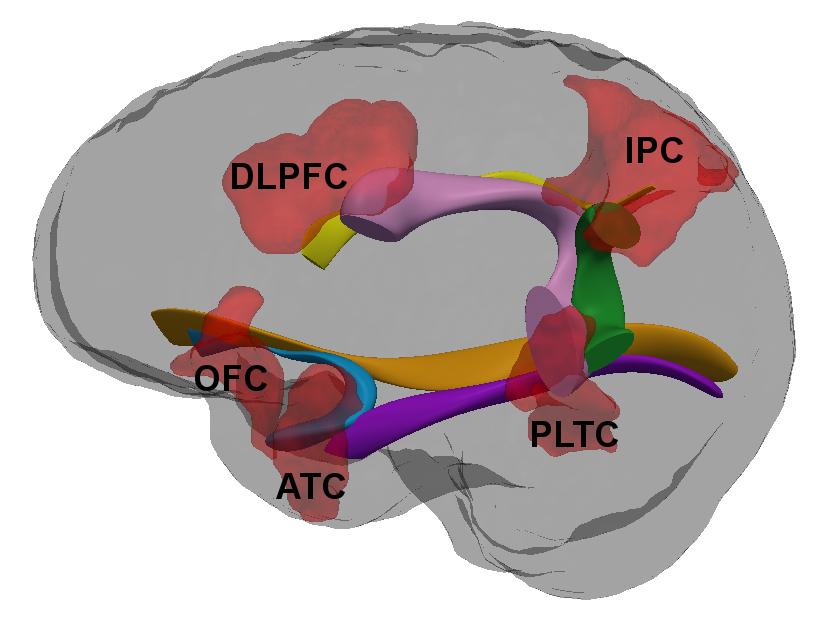
\includegraphics[width=1.0\linewidth]{figures/big_homo_labeled.png}
\caption{Functionally activated cortical regions (shown in red) were used to identify white matter fiber bundles that connected any two activated regions of interest. This resulted in the identification of the uncinate fasciculus (yellow), arcuate fasciculus (pink), inferior frontal-occiptal fasciculus (orange), inferior longitudinal fasciculus (purple), superior longitudinal fasciculus (light blue) and the arcuate fasciculus vertical (green)}
\label{fig:networkmodel}
\end{center}
\end{figure}

\begin{figure}[h]
\begin{center}
\begin{tabular}{c c}
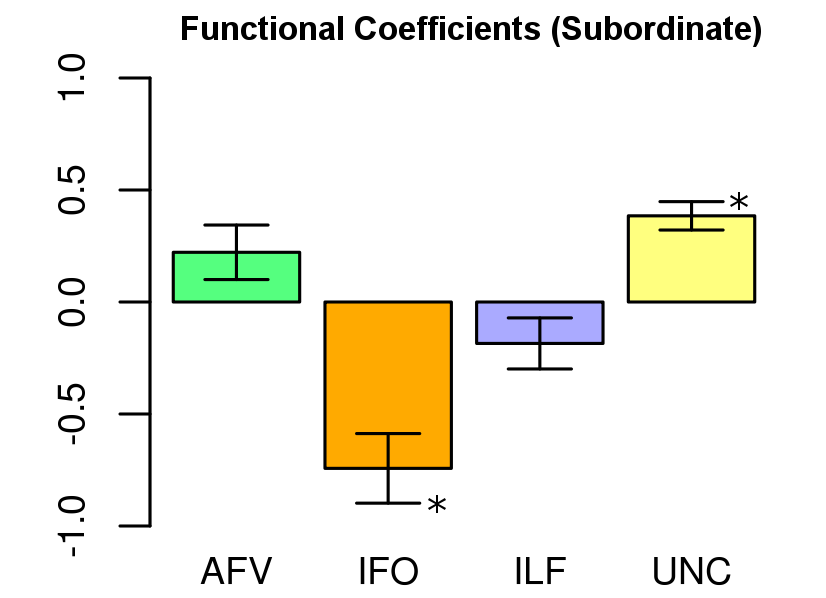
\includegraphics[width=0.45\linewidth]{figures/FC_Subordinate2.png} &
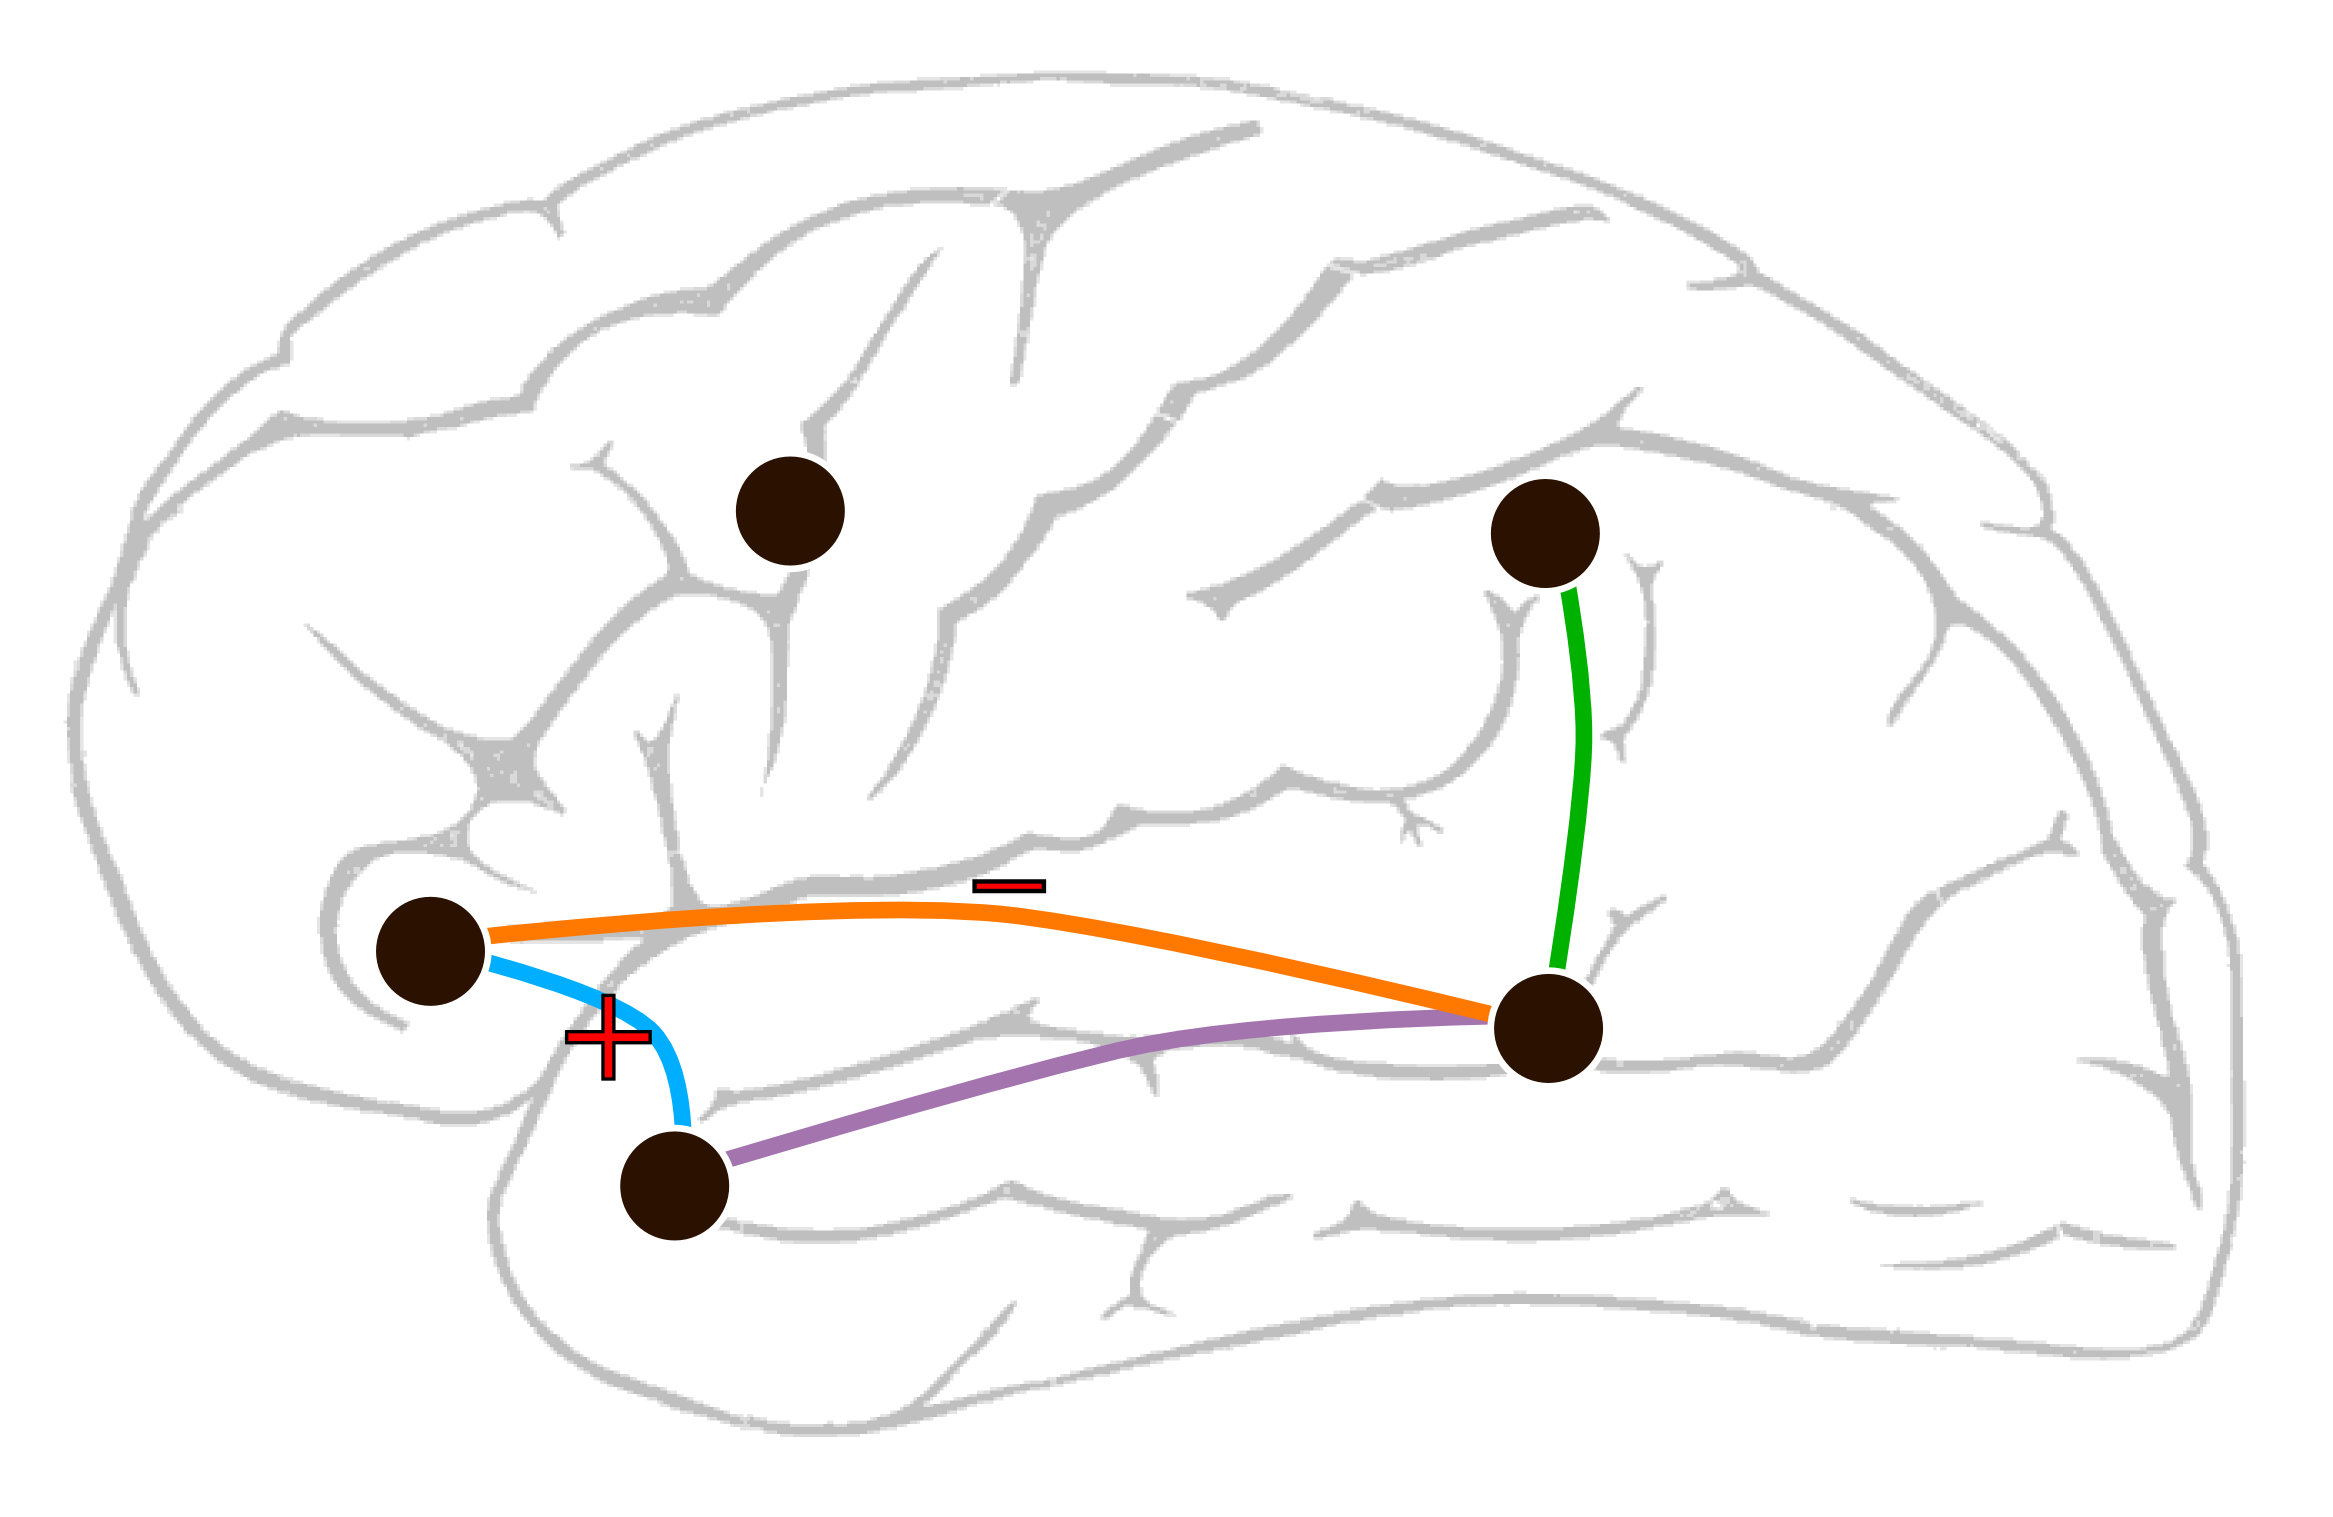
\includegraphics[width=0.45\linewidth]{figures/func_diag2.png}
\end{tabular}
\caption{Stepwise multiple linear regression analysis examining performance in the subordinate context and functional connectivity between regions connected by a white matter fiber tract resulted in a model including the vertical aspect of the arcuate fasciculus (AFV), IFO, IFL and UNC. * $p<0.05$}
\label{fig:mlr_fc}
\end{center}
\end{figure}

\begin{figure}[h]
\begin{center}
\begin{tabular}{c c}
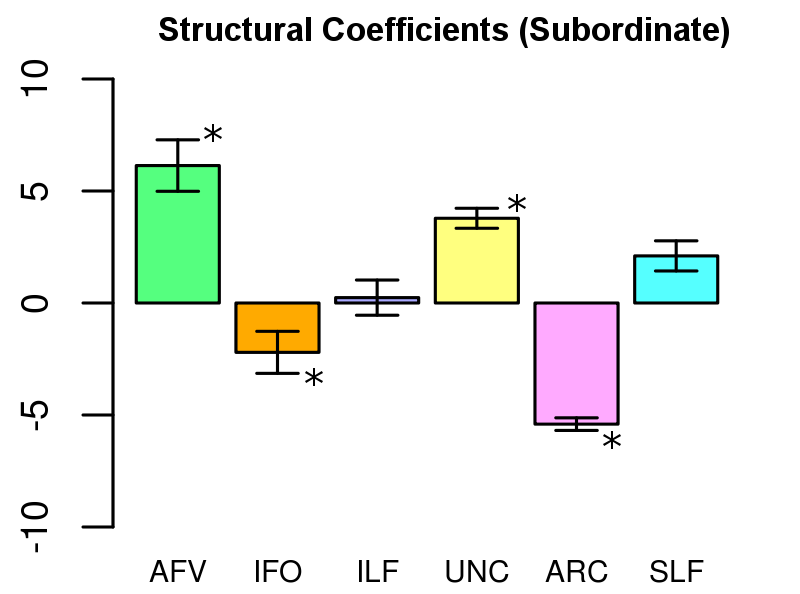
\includegraphics[width=0.45\linewidth]{figures/FA_Subordinate2.png} &
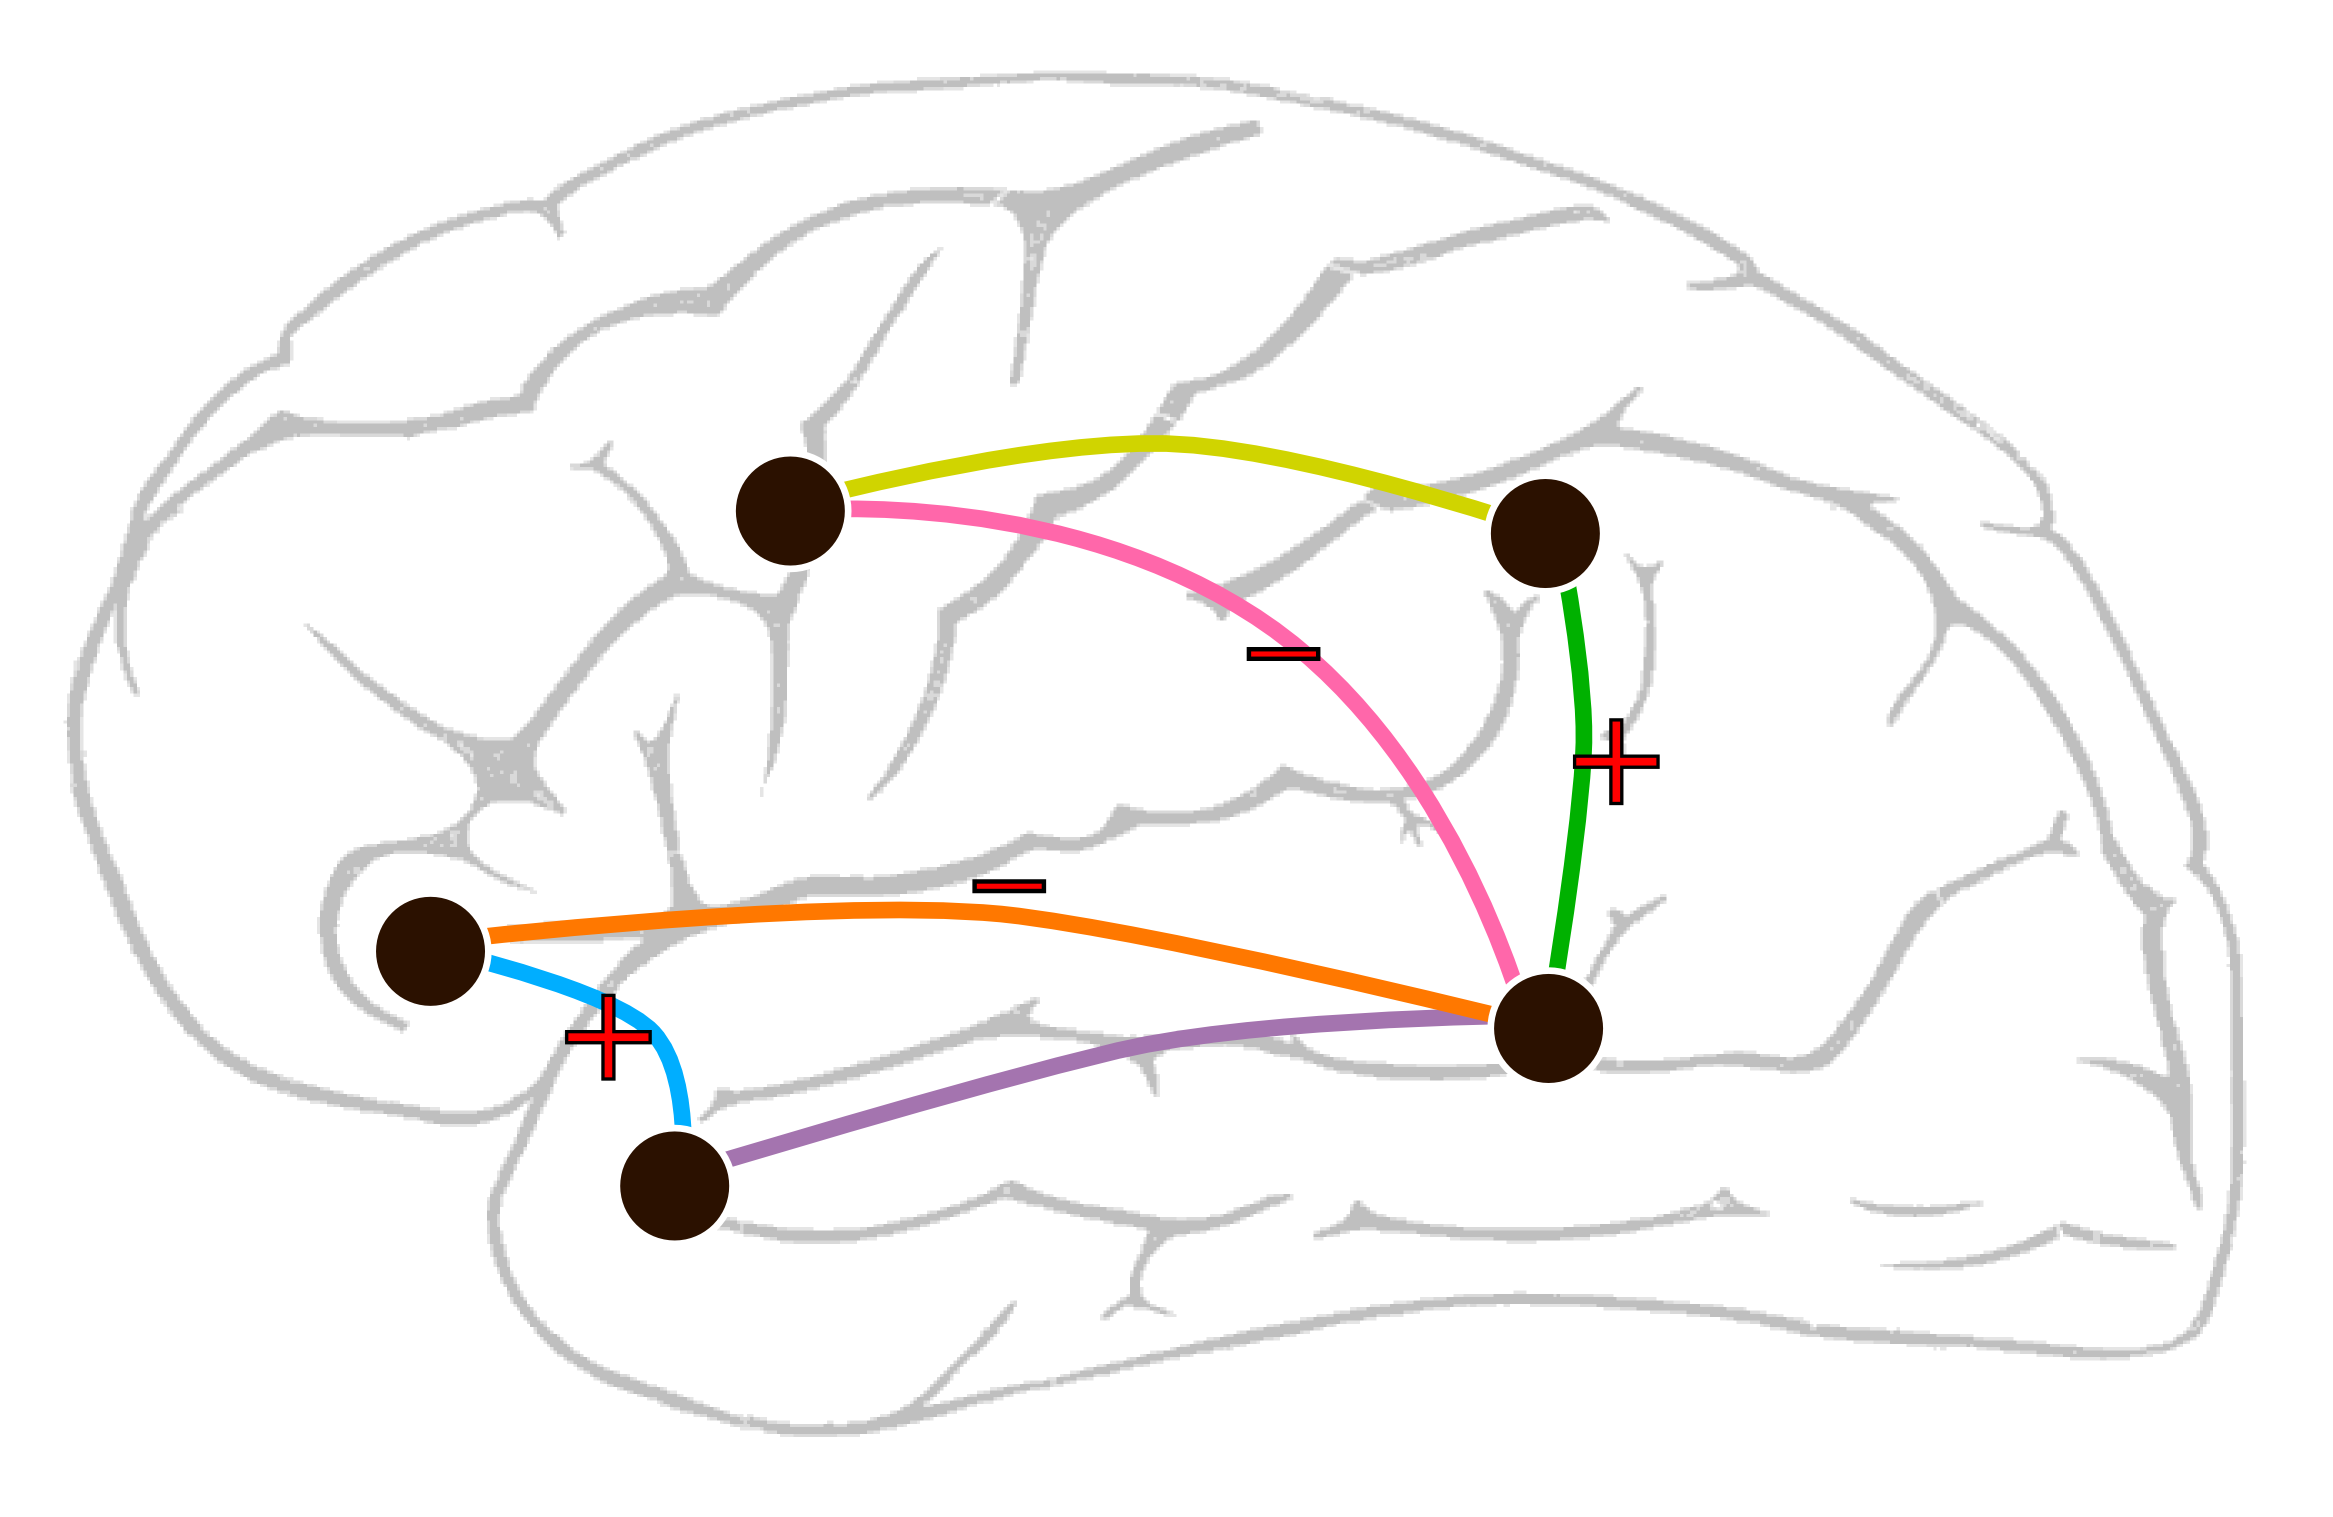
\includegraphics[width=0.45\linewidth]{figures/struct_diag2.png}
\end{tabular}
\caption{Stepwise multiple linear regression analysis examining performance in the subordinate context and tract averaged FA implicated all biological connections in the network: uncinate fasciculus (UNC), arcuate fasciculus (ARC), superior longitudinal fasciculus (SLF), inferior longitudinal fasciculus (ILF), inferior frontal-occipital fasciculus (IFO) and the arcuate fasciculus vertical (AFV). The coefficients for each structure are illustrated here. *Indicates an individually significant fiber tract ($p<0.05$).}
\label{fig:mlr_fa}
\end{center}
\end{figure}



\section{Functional Connectivity}
\label{appa}
\begin{table}[h]
\begin{center}
\tiny
\begin{tabular}{| l | r l | r l | r l |}
\hline
Regions & \multicolumn{2}{|c|}{Dominant} & \multicolumn{2}{|c|}{Neutral} & \multicolumn{2}{|c|}{Subordinate}\\
\hline
OFC $\leftrightarrow$ ATC &     (0.6) & $0.471 \pm 0.303$ &  (0.5) & $ 0.418 \pm 0.362$ &  (0.5) & $ 0.375 \pm 0.380$\\
ATC $\leftrightarrow$ PLTC &    (0.5) & $0.499 \pm 0.262$ &  (0.8) & $ 0.584 \pm 0.263$ &  (0.7) & $ 0.570 \pm 0.255$\\
OFC $\leftrightarrow$ PLTC &   (1.0) & $0.722 \pm 0.139$ &  (0.9) & $ 0.693 \pm 0.191$ &  (0.9) & $ 0.683 \pm 0.153$\\
PLTC $\leftrightarrow$ DLPFC & (1.0) & $0.701 \pm 0.010$ &  (0.9) & $ 0.671 \pm 0.164$ & (1.0)  & $ 0.686 \pm 0.126$\\
PLTC $\leftrightarrow$ IPC &    (0.7) & $0.488 \pm 0.287$ &  (0.6) & $ 0.484 \pm 0.300$ &  (0.6) & $ 0.493 \pm 0.236$\\
IPC $\leftrightarrow$ DLPFC &   (0.7) & $0.586 \pm 0.342$ &  (0.9) & $ 0.685 \pm 0.209$ &  (0.7) & $ 0.592 \pm 0.308$\\
\hline
\end{tabular}
\caption{Functional connectivity values between cortical ROIs with direct biological connections, as determined with DTI tractography. Cortical regions include orbital frontal (OFC), anterior temporal (ATC), posterior lateral temporal (PLTC), dorso-lateral prefrontal (DLFPC), and inferior partietal (IPC). The number in parentheses is the fraction of subjects that exhibited significant ($p < 0.05$) functional connectivity for that pair of regions. This is followed by the mean and standard deviation of the correlations for all subjects.}
\label{table:fcvalues}
\end{center}
\end{table}

\section{Fractional Anisotropy}
\label{appb}
\begin{table}[h]
\begin{center}
\begin{tabular}{| l | l |}
\hline
Structure & Average FA\\
\hline
Uncinate fasciculus & $ 0.397 \pm 0.092$\\
Inferior longitudinal fasciculus & $ 0.479 \pm 0.142$\\
Inferior fronto-occipital fasciculus & $ 0.646 \pm 0.122$\\
Arcuate fasciculus & $ 0.459 \pm 0.151$\\
Arcuate fasciculus (vertical) & $ 0.511 \pm 0.099$\\
Superior longitudinal fasciculus & $ 0.523 \pm 0.068$\\
\hline
\end{tabular}
\caption{Fractional anisotropy values in the white matter pathways that provide biological connectivity between the functional regions of interest.}
\label{table:connect}
\end{center}
\end{table}


% Background and Significance
% No page limit
\chapter{The lateralization of structure and function in aging: A combined fMRI and DTI study}
\label{chap_lat}

This chapter presents work submitted to the 13th International Conference on Medical Image Computing and Computer Assisted Intervention 2010 Workshop on Computational Diffusion MRI, Beijing, China. Measures from event-related functional MRI, diffusion tensor imaging tractography and cognitive performance in a language-based task were used to test the hypothesis that lateralization of function and structure changes with age and plays a role in regulating cognitive performance.  Functional activation was examined in three functionally activated regions and their opposite hemisphere homologues in healthy young adults and healthy seniors. The health seniors were divided into two groups, one that was cognitively matched with the young adults, and one that performed more poorly on a working memory task. The functional regions were used to identify the white matter fiber tracts that provide the biological connectivity between the activated regions and structural connectivity was measured by averaging fractional anisotropy (FA) over a geometric fiber bundle model that projects local white matter properties onto a centerline. Young adults had symmetric activation patterns. Seniors were found to have higher activation in the right posterior temporal cortex and this activation was higher for higher performing seniors than lower performing seniors. FA in the right hemisphere arcuate fasciculus was found to have higher FA in seniors, but lower FA was found in the right hemisphere short frontal fibers and the posterolateral temporal inter-hemispheric connections of seniors. Higher performing seniors also lower FA in the inferior frontal inter-hemispheric connections compared to lower performing seniors. Right hemisphere compensatory activation in older adults may be due in part to age-related changes in white matter connectivity.


\section{Introduction}
\label{sec:intro}
Lateralization, the asymmetric distribution of cognitive resources between hemispheres, is a distinctive feature of the human brain. The first evidence for functional lateralization was provided by Paul Broca's (1824 - 1880) post-mortem examinations of subjects with language deficits which revealed that the left hemisphere subserves language processing. More detailed examinations of lateralization were conducted by Roger Sperry~\cite{Sperry1974} who conducted a series of experiments testing functional lateralization in subjects whose corpus callosa had been surgically severed in order to prevent epileptic seizures. These experiments demonstrated that when words were presented to the left visual field (i.e. right hemisphere), the subjects did not report seeing anything, but when the words were presented to the right visual field, the subjects were able to correctly report the word. More recently, functional magnetic resonance imaging (fMRI) has provided further evidence confirming that language processing is handled in the left hemisphere~\cite{Frost1999,Bookheimer2002}. Addtionally, diffusion tensor imaging (DTI) tractography has been used to identify hemispheric asymmetries in the white matter tracts that provide the anatomical connections between the cortical regions associated with the language network~\cite{Catani2008,Glasser2008}.
 
Studies of the aging brain have suggested that older adults recruit right hemisphere resources for language processing, however the basis for the compensatory process is not known~\cite{Cabeza2002}. A number of hypotheses have been proposed to explain the changes in functional lateralization that accompany aging. The \emph{compensation view} posits that increased right hemispheric activity is an attempt to counteract age-related neurocognitive decline~\cite{Cabeza1997} whereas the \emph{dedifferentiation view} posits that these increases are are the result of a response to increased difficulty in the recruiting of specialized neural mechanisms~\cite{Li1999}. The \emph{psychogenic view} posits that these changes reflect the implementation of novel cognitive strategies that are not used (and not needed) by younger adults except for very difficult tasks~\cite{Light1991}. This contrasts with the \emph{neurogenic view} which posits that the asymmetry reductions a the result of age-related changes to neuronal architecture. A global reorganization of functional specialization is posited by the \emph{network view} while the \emph{regional view} posits that the asymmetry changes are independent of functional specialization. The \emph{resources view} posits that cognitive processes are fueled by limited resources and that decreased lateralization results from age-related capacity declines in left-hemispheric neural units~\cite{Craik1983}. An age-related decline is processing speed is assumed by the \emph{speed view} which posits that increased recruitment of neurons results in increased processing speed. Finally, the \emph{inhibition view} posits that age-related declines in inhibition result in reduced lateralization resulting in decreased cognitive performance due to greater influence of task-unrelated information~\cite{Hasher1988}. Many of these views are not mutually exclusive, suggesting that the true origin for reduced functional lateralization may be some combination of the above. The evaluation of these views is complicated by a lack of information regarding: the relationship of lateralization and cognitive performance with aging, incidence and age-of onset of decreased lateralization, and gender differences.

To gain further insight into the nature of lateralization changes with aging it is necessary to not only examine functional activity in the brain, but also the structural properties in the biological network that provides the connections that allow inter-hemispheric communication. These inter-hemispheric, or commisural, connections are provide by the corpus callosum, the largest neural pathway in the human brain, incorporating between 200 million and 800 million axons~\cite{Banich1995}. The corpus callosum consists primarily of homotopic connections that connect homolous cortical regions in each hemisphere~\cite{Hellige1993}, but evidence has been found for a small number of heterotopic connections~\cite{Wahl2009}. Studies of the corpus callosum often treat it is a single entity, but previous studies have revealed that different components of the corpus callosum transfer different types of information suggesting that the corpus callosum may be more accurately depicted as a collection of independent pathways~\cite{Banich1995}. The functional role of the corpus callosum is still an open issue with evidence for both inhibitory and excitatory roles~\cite{Yazgan1995}. The balance between inhibition and excitation may be regulated by a balance between the two fiber types that make up the corpus callosum, large diameter fibers that connect sensory-motor areas and small diameter fibers that connect association areas~\cite{Yazgan1995}. The smaller diameter axons are more prevalent and are believed to responsible for individual differences in callosal size~\cite{Bloom2005}. 

In this study, functional subnetworks in the brain were examined using MRI to measure both structure and function during a language processing task. A healthy young adult population was compared to healthy seniors. The seniors were grouped into higher performing and lower performing groups so that functional and structural differences could be examined. Functional regions identified in a previous study~\cite{Gunawardena2009} were used to examine region-averaged activation values. The functional regions were then used to identify the white matter fiber tracts that provide the communication channels between the functional regions. Atlas-based DTI tractography was used to create geometric models of fiber bundles. Deterministic tractography was used to identify the well defined association fibers that connect the functional regions of interest while a shortest-path tractography method is used to identify the inter-hemispheric connections. Structure was quantified with arc-length parameterizations of fractional anisotropy (FA)~\cite{Jones2005,Corouge2006,Maddah2008d,ODonnell2009}. These structural and functional metrics were used to identify possible differences between the young adult and senior populations as well as within the high and low performing senior groups.

\section{Methods}
\label{sec:methods}
Functionally activated regions were defined using fMRI and used to examine functional activation levels in these regions as well as in homologous regions in the opposite hemisphere. The activated regions were used along with diffusion tensor MRI tractography to identify the white matter pathways that provide the biological connectivity of the network. Tract-averaged FA was measured in each fiber tract using a centerline-based method to identify structural differences related to aging. Diffusion tensor images, T1 images and fMRI were acquired for a set of ten young adults and 13 seniors. A working memory test was used to group the seniors into two sets, one that was cognitively matched with the young adults (n=7), and one that performed more poorly on the test (n=6). These groupings are used to examine the relationship between structure and function and their relationship to cognitive performance and aging. 

\subsection{Analyses of fMRI}
A previous study investigated the neural mechanisms that support the resolution of grammatically complex sentences~\cite{Gunawardena2009}. Regions were identified from a contrast of the point at which an ambiguity is encountered in a sentence with a  ``more-compatible" direct object structure (e.g. ``The mayor heard the election result on the radio") minus ``less-compatible" sentences (e.g. ``The mayor heard the election result was fixed")~\cite{Gunawardena2009}. 

Processing of the fMRI data was performed using SPM5~\cite{SPM5}. For each subject, the functional data was motion-corrected, transformed into MNI space, spatially smoothed with a 8mm FWHM isotropic Gaussian kernel and interpolated to isotropic 2 mm voxels. A canonical hemodynamic response function was used to convolve the onset times of stimulus events for each condition. A general linear model approach was then used to calculate statistical parameter estimates for each subject. The previously identified cortical regions were used to determine a peak activation MNI-space coordinate which was used as the center of a spherical region of interest (ROI) with a radius of 8mm. The regions are listed in table~\ref{table:coords}. The activated regions were located in the left-hemisphere. Right hemisphere homologous regions were identified in order to examine functional lateralization. An average t-value was calculated for each ROI, in each subject. 

\begin{table}[h]
\begin{center}
\begin{tabular}{| l | l l l |}
\hline
Cortical Region & \multicolumn{3}{c |}{MNI Coordinates} \\ 
\hline
Dorso-lateral prefrontal (DLPFC) & -48 & 16 & 34\\
Posterior lateral temporal (PLTC) & -58 & -44 & 0 \\
Inferior frontal (IPC) & -48 & 8 & 12\\
\hline
\end{tabular}
\caption{Peak activation MNI coordinates of functional regions of interest}
\label{table:coords}
\end{center}
\end{table}

\subsection{Analyses of DTI}
Diffusion tensor tractography in individual subjects is highly subject to false-positive connections, but recent work has shown that population atlases provide an appropriate space for identifying fiber bundle geometry~\cite{Goodlett2009a,Yushkevich2008,Smith2006}. To achieve this, a multivariate atlas was created for the young and elderly subjects from larger data sets of scanner and age-matched subjects. The young and elderly atlases were then registered into a single final template space. Each subject's high resolution T1 weighted image was registered to the corresponding age-matched template using Symmetric Normalization as implemented in Advanced Normalization Tools~\cite{Avants2006}. This was accomplished through the use of a multi-resolution, non-rigid registration algorithm to optimize a cross correlation metric under the constraints of a diffeomorphic transformation model~\cite{Avants2006}. A brain mask of the template was propagated to each subject's T1 weighted image.  These skull-stripped T1 weighted images were then registered to the FA image derived from each subject's diffusion tensor image. The intra-subject transforms were composed with the T1 atlas transforms in order to transform the each subjects' tensor data into the final template space using the preservation of principle technique along with log-Euclidean linear interpolation. 

\subsection{Fiber Tractography}
The diffusion tensor component of the atlas was used to perform whole brain, deterministic fiber tractography~\cite{Cook2006}. Landmarks were manually placed in the T1 component of the atlas in order to extract well defined white matter fiber bundles~\cite{Wakana2004}. The functionally activated regions were warped from MNI space into the template space and used as target regions to identify fiber bundles that connected two regions of interest. Deterministic tractography was sufficient for identifying the association fibers that provide the intra-hemispheric connections, but was not sufficient for identifying the inter-hemispheric connections (see figure ~\ref{fig:callosum}). Deterministic DTI tractography is known to have difficulty distinguishing between multiple fiber directions in a single voxel and is biased towards the most prominent fiber direction in a voxel. In the case of the corpus callosum, deterministic DTI tractography only identifies inter-hemispheric connections between superior cortical regions. To identify the most likely connective pathways between the lateral cortical regions examined here, a shortest-path methodology was employed. The total cost of a given potential pathway is determined by examining a local energy metric, $f(x)$, and summing over all points $x$ in the path. 
\begin{equation}
f(x) = \beta_1 d(x,x-1) + \beta_2 (1.0 - FA(x)) + \beta_3 (1.0 - \vec{e(x)}\vec{t(x)} )
\end{equation}
where $d(x,x-1)$ is the distance between $x$ and the previous position of $x$, $FA(x)$ is the fractional anisotropy of the tensor at $x$, $\vec{e(x)}$ is the principle direction of diffusion at $x$, $\vec{t(x)}$ is the tangent to the path at $x$, and $\beta_1$, $\beta_2$ and $\beta_3$ are user controlled parameters (here we used $\beta_1 = 1.0$, $\beta_2 = 3.0$, and $\beta_3 = 1.0$). Dijkstra's algorithm is used to find the shortest-path between a seed point and a set of possible target points~\cite{Dijkstra1959}. To find the fiber tracts that provide inter-hemispheric connectivity, all points in each left hemisphere region were used as seeds and the points in the homologous right hemisphere region were used as possible targets. The process was then repeated using the right hemisphere as seeds and the left hemisphere points as targets. For each pair of regions this resulted in a set of streamlines connecting the regions.

\begin{figure}
\begin{center}
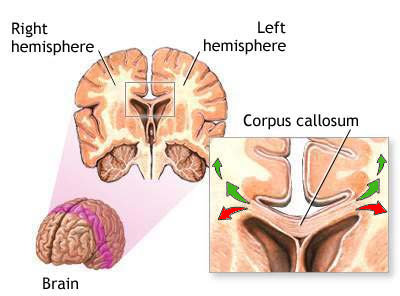
\includegraphics[width=0.5\linewidth]{figures/corpus_callosum_lateral.png} \\
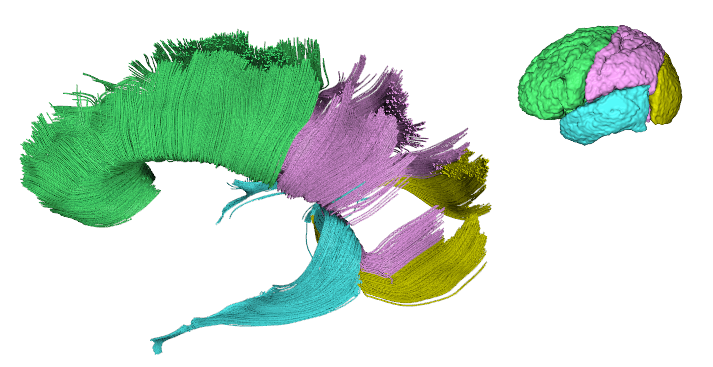
\includegraphics[width=0.8\linewidth]{figures/ccfibers2.png}
\caption{Above: The human corpus callosum (image adapted from~\cite{medlineplus}). Deterministic tractography methods are able to identify the aspects of the corpus callosum that connect superior cortical regions (green arrows), but are unable to identify the aspects that extend to more lateral cortical regions (red arrows). Below: Example results of atlas-based deterministic fiber tractography of the human corpus callosum with fibers colored by brain lobe. }
\label{fig:callosum}
\end{center}
\end{figure}

A centerline or skeletonization technique provides a method for avoiding bias caused by partial voluming that occurs in voxels that are not entirely within the white matter of the fiber tract of interest~\cite{Smith2006,Yushkevich2008}. Here we used a template-fiber approach. Each white matter tract was estimated as a set of streamlines, each of which was parametrized by arc-length to extend from 0.0 to 1.0. A BSpline was then fit to the set of all points from all streamlines in each bundle to obtain a single centerline that lies in the core of the fiber pathway of interest. For each point along the model pathway, a tangent was calculated and used to determine a perpendicular plane. The intersection of this plane with each of the streamlines in the bundle defined a set of points.  The normal and binormal vectors were used to re-parameterize the intersection points into 2D coordinates. Graham's scan method was used to determine the convex hull that encloses the set of intersection points~\cite{Graham1972}, and least-squared method was applied to the points on the hull to define an elliptical cross-section~\cite{Fitzgibbon1999}. To obtain a single FA value for the entire fiber bundle, the FA values were averaged over the length of the centerline.

\section{Results}

\subsection{Function}
The functional analyses revealed a network made up of 3 activated regions in the left hemisphere: dorsolateral prefrontal cortex (DLPFC), posterolateral temporal cortex (PLTC) and inferior frontal cortex (IFC). The region-averaged functional activation values are summarized in figure~\ref{fig:activations}. To identify activation changes that potentially result from aging, a Student's t-test was used to compare the young adults to all seniors for each ROI and suggested that activation in the right posterolateral cortex is greater in seniors (p=0.012). This same approach was used to identify potential differences between the cognitively matched and unmatched seniors. The cognitively matched seniors were found to have greater activation in the right dorsolateral prefrontal cortex (p=0.014) and reduced activation in the left posterolateral cortex (p=0.033) compared to the unmatched seniors.

\begin{figure}
\begin{center}
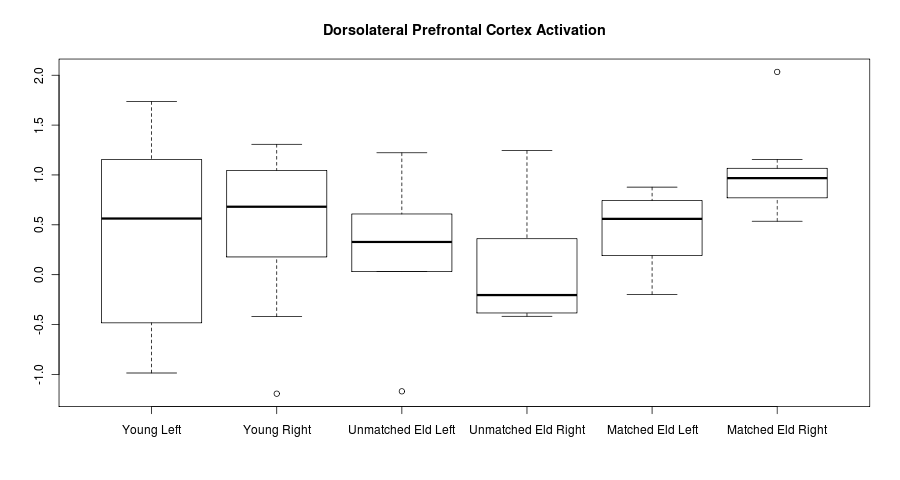
\includegraphics[width=0.8\linewidth]{figures/dlc_activation.png}\\
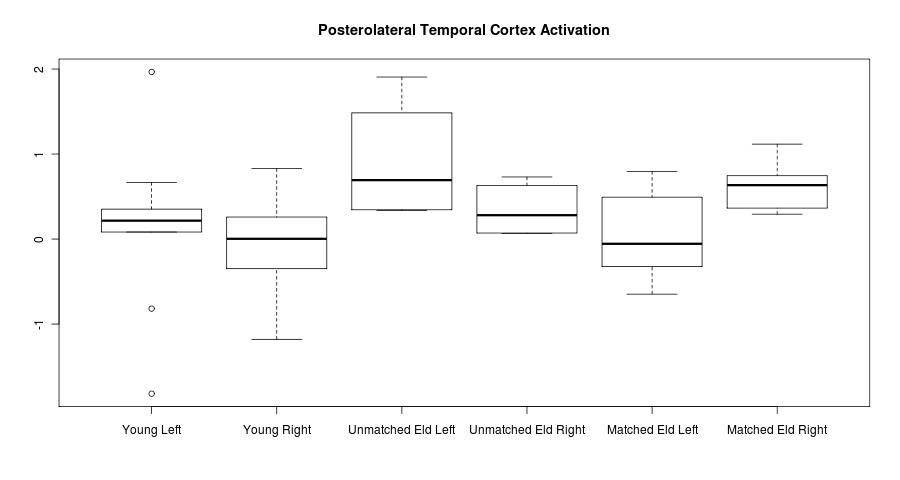
\includegraphics[width=0.8\linewidth]{figures/ptc_activation.png}\\
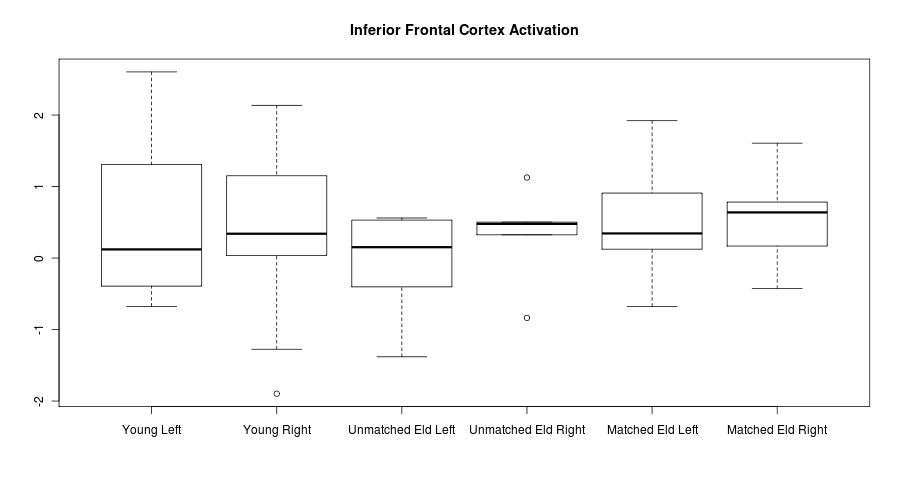
\includegraphics[width=0.8\linewidth]{figures/ifc_activation.png}
\caption{Region-averaged functional activation was measured in both hemispheres in the dorsolateral prefrontal cortex (top row), posterolateral temporal cortex (middle row) and inferior frontal cortex (bottom row).}
\label{fig:activations}
\end{center}
\end{figure}

\subsection{Structure}
The DTI tractography identified a network of connections made up of the arcuate fasciculus (right and left hemispheres), a bundle of short frontal fibers (right and left hemispheres), and 3 subcomponents of the corpus callosum. These fiber bundles were used to generate geometric models, illustrated in figure~\ref{fig:fibers}. A Student's t-test was used to identify potential differences between the young adults in seniors. Reduced FA in seniors compared to young adults was found in the inter-hemispheric connection between the PLTC regions (p=0.02889) and in the right short frontal fibers (p=0.00955). Increased FA in seniors was found in the right arcuate fasciculus (p=0.00747). Compared to lower performing seniors, higher performing seniors had lower FA in the inter-hemispheric connections between right and left IFC. 

\begin{figure}
\begin{center}
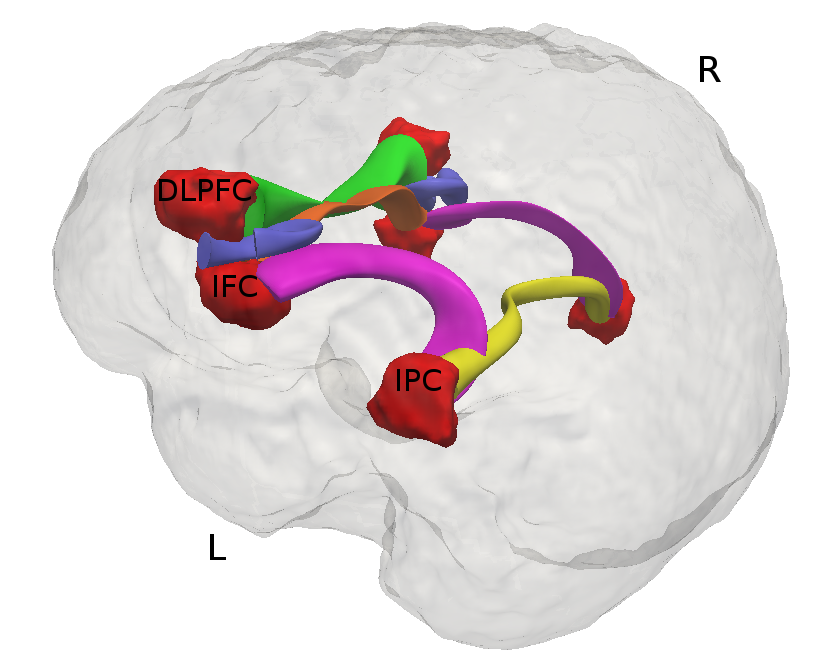
\includegraphics[width=0.9\linewidth]{figures/big_lat_labeled.png}
\caption{A set of 3 functionally activated regions: Dorsolateral Prefrontal Cortex (DLPFC), Posterolateral Temporal Cortex (PLTC), and Inferior Frontal Cortex (IFC) were identified in the left hemisphere. These regions, along with their right hemisphere homologues were used to identify the fiber tracts that provide biological connectivity. In each hemisphere, intra-hemispheric connectivity is provided by the arcuate fasciculus (pink) and a bundle of short frontal fibers (blue). Each homologous pair of activated regions was used to identify the following subcomponents of the corpus callosum that provided inter-hemispheric connectivity: DLPFC (green), IFC (orange) and PLTC (yellow). Surface-meshes created from the the geometric models are used for visualization of the white matter tracts.}
\label{fig:fibers}
\end{center}
\end{figure}

\begin{figure}
\begin{center}
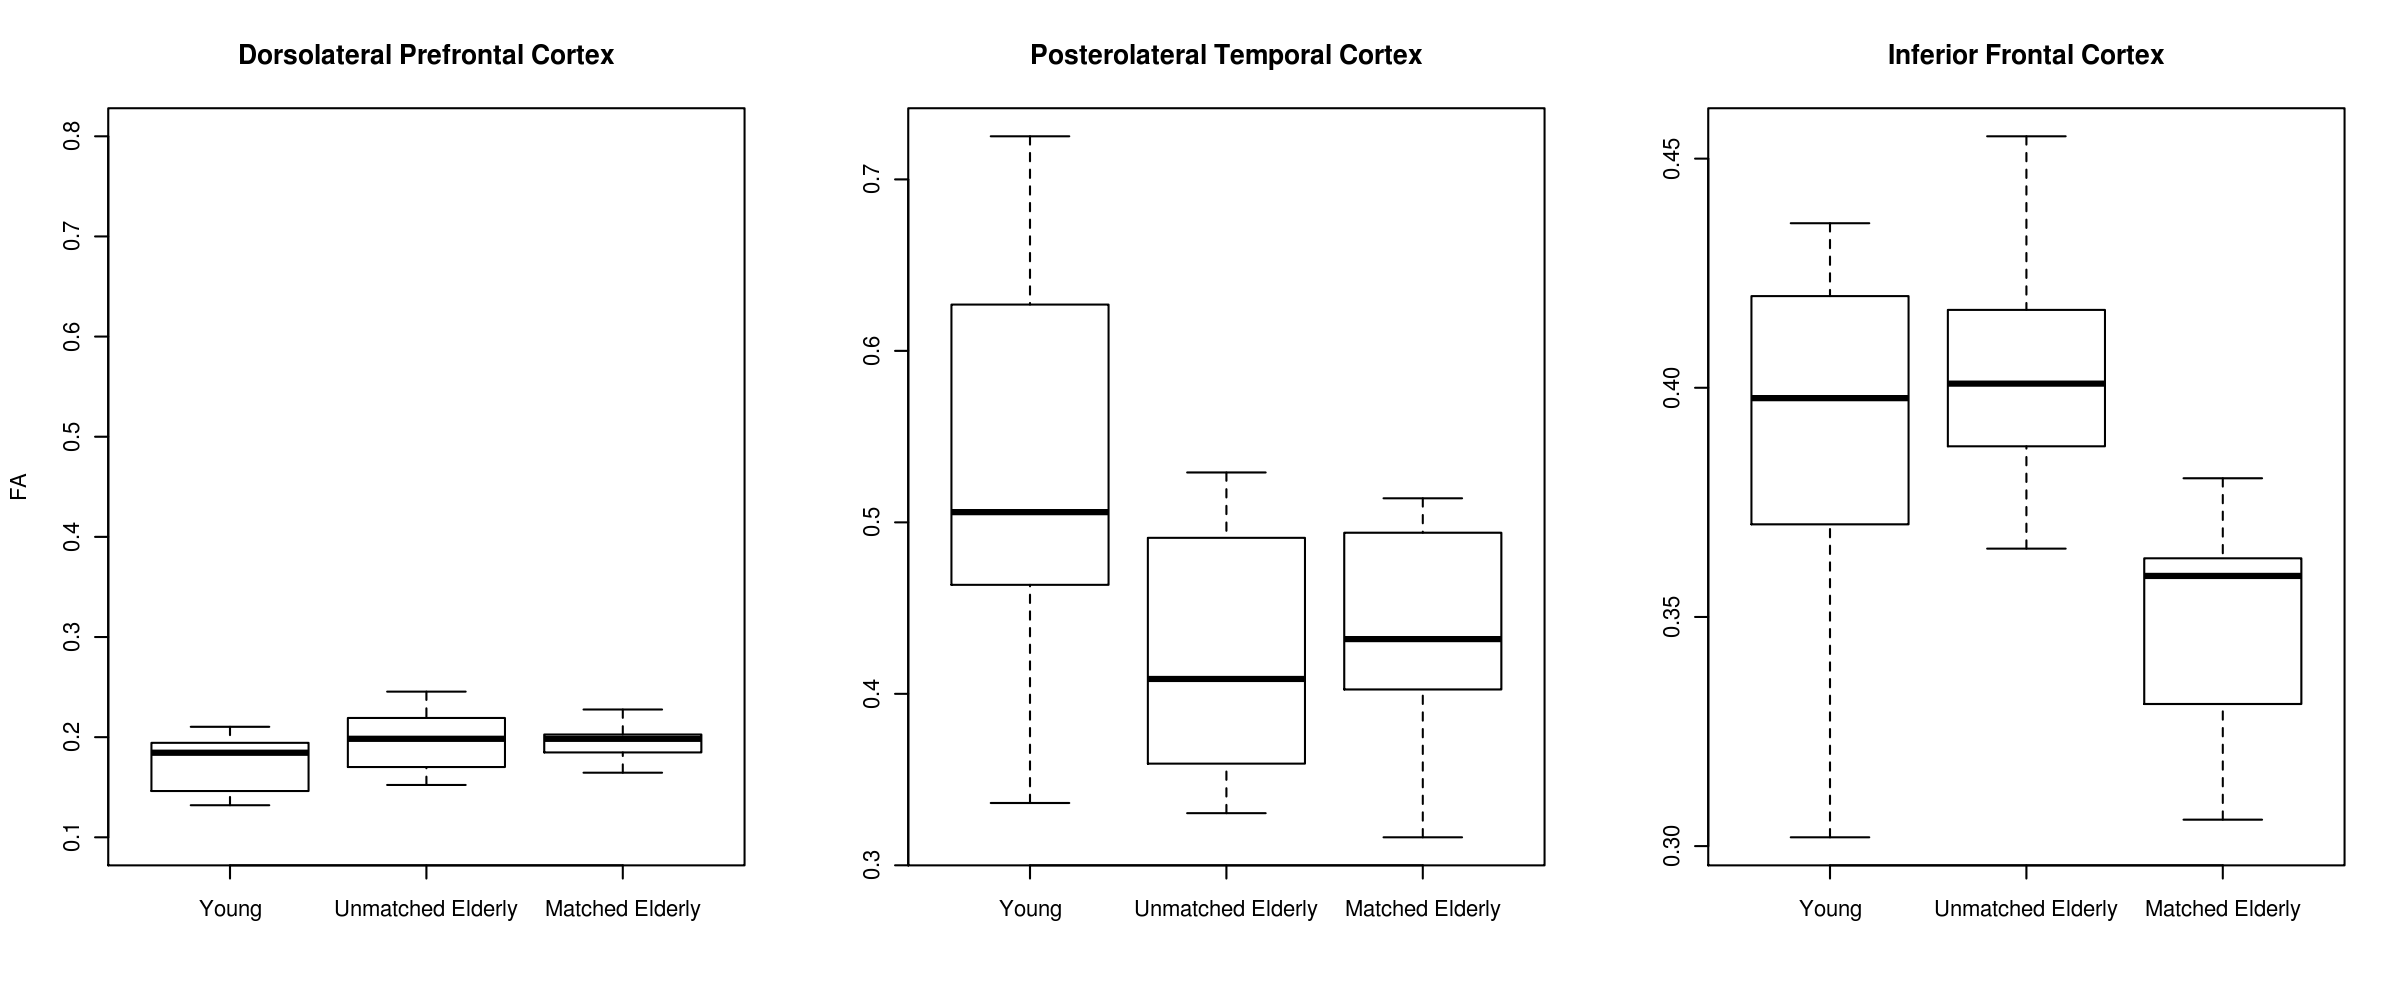
\includegraphics[width=1.0\linewidth]{figures/commissural.png}\\
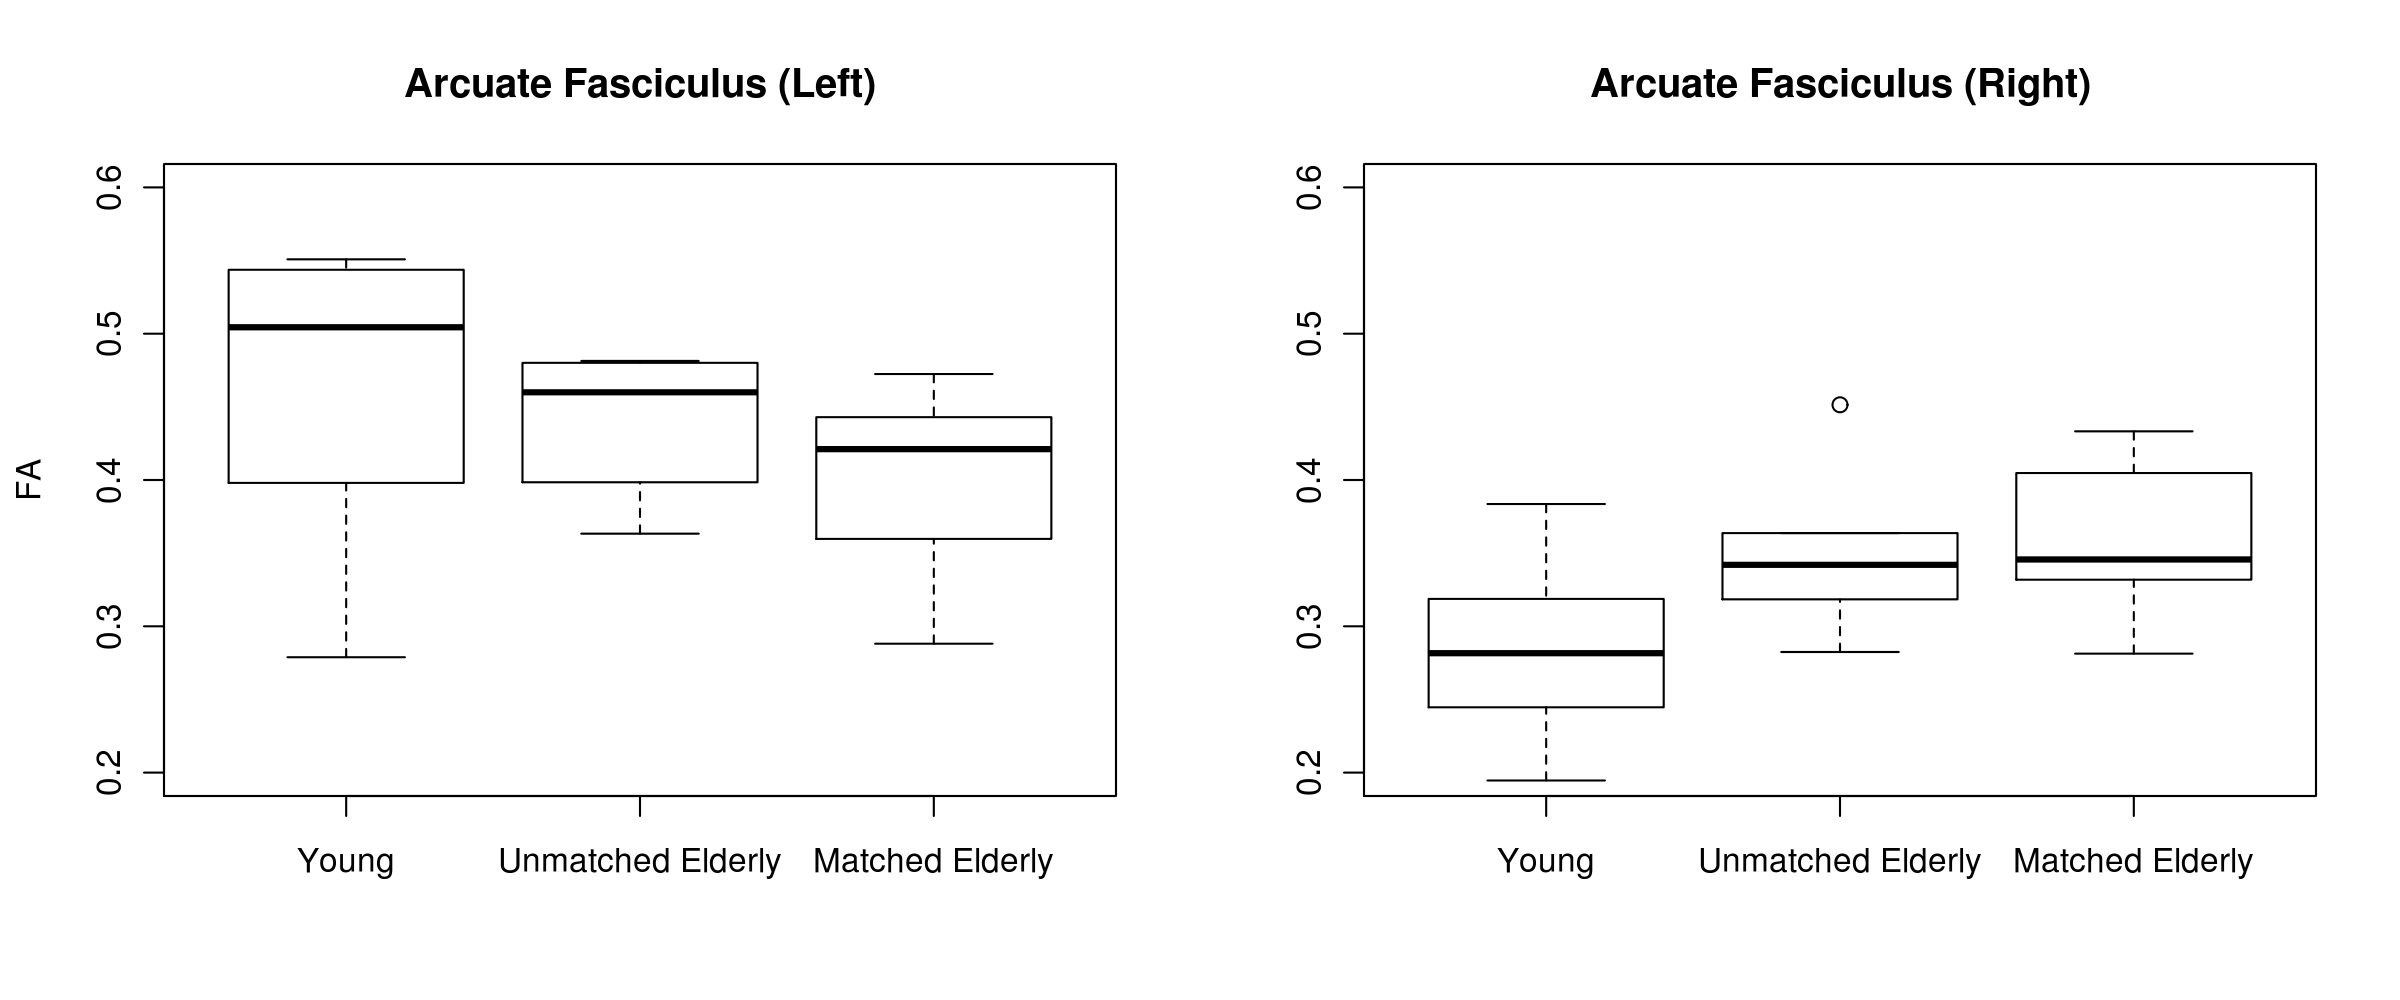
\includegraphics[width=0.8\linewidth]{figures/arcuate.png}\\
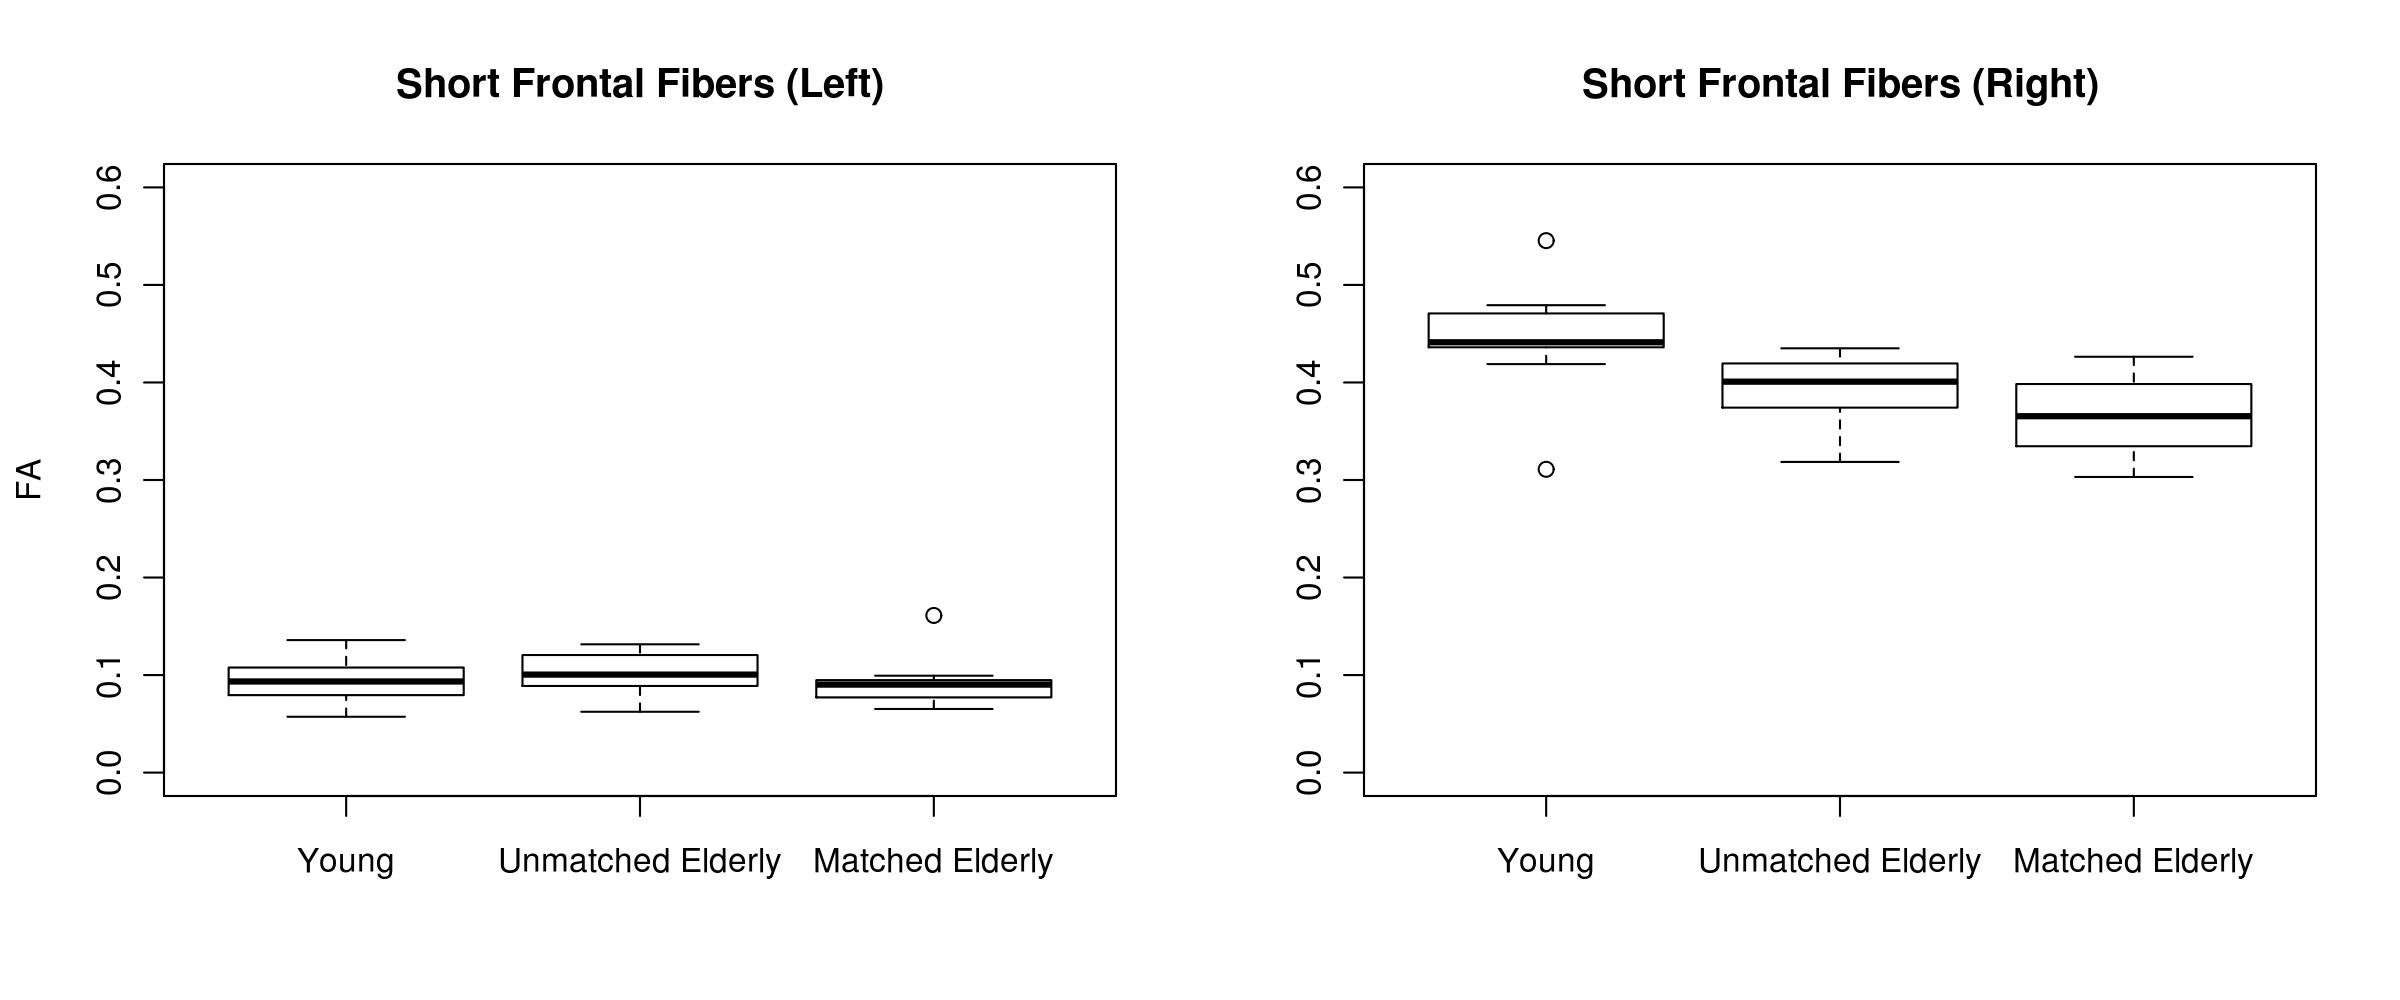
\includegraphics[width=0.8\linewidth]{figures/short.png}
\caption{Tract-averaged fractional anisotropy was measured for the portions of the corpus callosum that provide inter-hemispheric connections between the cortical regions of interest (top row), the arcuate fasciculus (middle row) and short frontal fibers (bottom row). }
\label{fig:fa}
\end{center}
\end{figure}

\section{Discussion}
This study demonstrated the potential for using combined analysis of fMRI and DTI in examining age-related changes in function and structure in the brain and how these changes regulate behavior. While language processing is primarily handled in the left hemisphere, the activation in young adults was symmetric. This is possibly a result of younger adults having an easier time processing the grammatically complex sentences due to intact neural resources. The finding of increased activation in the right PLTC of seniors is consistent with the \emph{compensation view} that right hemisphere brain function during language processing increases with age~\cite{Cabeza2002}. Also supporting this view is the finding of higher activation in the right DLPFC of higher performing (matched) seniors relative to lower performing (unmatched) seniors. The finding of increased left PLTC activation in lower performing seniors is also interesting in the context of activation patterns. Examining figure~\ref{fig:activations} reveals that lower performing seniors have a similar activation pattern to that of young adults (higher in left than right) with higher overall activation values. Higher performing seniors however have a different activation pattern (higher in right than left) suggesting that recruitment of right hemisphere resources is a more effective strategy for compensating for the effects of aging than maintaining a similar pattern to the young adult brain and increasing activation, supporting the \emph{psychogenic view}. While these results are interesting, the small number of subjects limited the scope of the study, and many of the findings would not stand-up to a family-wide (FWE) error correction. 

The finding of increased FA in the right hemispheric arcuate fasciculus and deceased FA in the short frontal fibers in the right hemisphere suggests that the increased functional recruitment of right hemispheric resources may be accompanied by white matter changes. The finding of reduced FA in the inter-hemispheric connections is also consistent with the \emph{compensation view} as these connections are thought to play an inhibitory role that aids in hemispheric specialization~\cite{Yazgan1995}. This is additionally supported by the finding of reduced FA in the PLTC connections of higher performing seniors compared to lower performing seniors who have similar FA values to those in young adults. However, due to the complicated composition of the corpus callosum, caution must be taken when interpreting FA values as FA is sensitive to a variety of white matte properties including but not limited to: myelination, axon diameter and density, fiber tract curvature, and intra-voxel fiber crossings~\cite{Barkovich2000,Shimony1999,Virta1999}. All of these factors are relevant in the corpus callosum which contains two different types of fibers (i.e. small diameter and large diameter) that make up independent subcomponents that may vary in density and degree of myelination and connect to different functionally specialized cortical regions. While our examination attempted to focus on connections between association regions, the mixing of fibers that occurs as fiber approach the mid-sagittal cross-section could cause a partial voluming bias based upon myelination differences in sensory-motor fibers. As demonstrated by Pierpaoli et al.\ \cite{Pierpaoli2001}, a selective decrease in the FA of one fiber population may result in an increase in FA within an individual voxel, and vice versa. Because of these issues, more work must be done to gain a deeper understanding of the physical basis for the structural changes detected here.

The use of template fibers with elliptical cross-sections provided an effective geometric model for examining white matter fiber bundle properties, and a great deal of opportunity exists for the development of more biologically relevant measures of structure. Here, these models were purely template-based and used to examine FA in individual subjects. Using these template-based models as a basis for fitting subject-specific models from subject-space tractography could potentially provide a more sensitive measure of structural integrity and could provide a framework that explicitly examines the geometry of white matter pathways as well as the properties of the underlying tissue. Additionally, the use of metrics that leverage the expected fiber orientation provided by the geometric model may be useful as they incorporate more widespread information about the fiber tract as opposed to the purely local measure provide by FA~\cite{duda08miccai}.

In order to examine functional activation in each hemisphere and identity connective pathways of the corpus callosum, cortical ROI's of equal volume were used. This is potentially problematic as language related regions such as Broca's area have been demonstrated to be larger in the left hemisphere and additionally varies a great deal between individuals~\cite{Galaburda1995}. This could potentially be addressed by incorporating the use of a cortical atlas in which cortical areas, such as Brodmann's areas, have been labeled. The use of a shortest-path fiber tracking method is dependent upon the a priori assumption that the target and seed regions are directly connected by a white matter tract. The low FA values found for the commisural connection of the DLPFC may suggest that rather than a direct connection, these regions may communicate via indirect connections via a combination of association and commisural fibers. 

In summary, an atlas-based approach was used to examine age-related changes in functional and structural lateralization. Seniors were found to have higher activation in the right PLTC and this activation was greater for higher performing seniors than lower performing seniors. Age-related increases and decreases in association fiber were found with FA in the right hemisphere arcuate fasciculus being higher in seniors, but FA in the right hemisphere short frontal fibers being lower in seniors. Reduced FA was found in the the posterolateral temporal inter-hemispheric connections of all seniors. Differences were found between high and low performing seniors in the commisural connections of the IFC with low performing seniors having FA values similar to the young adults and high performing seniors having reduced FA. These results suggests that age-related changes in both functional and structural lateralization have effects on cognitive performance, but the limited sample size and complex nature of the structures requires further examination.










% Background and Significance
% No page limit
\chapter{Conclusions and Future Directions}
\label{chap_conclusions}

\section{Contributions}
The specific contribution of this dissertation are as follows:
\begin{itemize}
\item We presented methods for using multivariate data to identify anatomy-specific white matter trajectories for the examination of focal white matter degradation resulting from traumatic brain injury.
\item A method for creating geometric models of tube-like fiber tracts was developed to increase statistical power and reduce dimensionality.
\item We undertook the first study demonstrating the cognitive influence of the functional and structural connections that integrate two subnetwork to form a large-scale neural network that allows for complex cognitive processing in a study of decision-making in a language task.
\item A study examining structure and function examined the hypothesis that a reduction in functional symmetry with aging is accompanied by structural changes in the fiber tracts that provide associative and commisural connectivity to the cortical regions associated with the language network.
\end{itemize}

\section{Future Directions}
In all methodological development, an emphasis was placed upon the the use of freely available, open-source code, specifically: ITK~\cite{Yoo2002}, ANTS~\cite{ANTS}, Pipedream~\cite{Pipedream} and Camino~\cite{Cook2006}. All relevant code will be integrated into these existing packages, and made publicly available. 

We have demonstrated a method for creating atlas-based geometric models of fiber tracts that is applicable to components of all fiber types found in the brain: projection, commissural and association. The creation of a single multivariate atlas in which all of these fiber tracts were identified and modeled could provide a basis for a number of studies. Evidence of effects in all of these fiber types has been found for TBI~\cite{duda08mmbia,Sidaros2008,Karunanayaka2007} and for aging~\cite{Ardekani2007,Salat2005,Bastin2010}.

Chapter~\ref{chap_tbi} presented evidence that subject-specific fitting of fiber templates enhances fidelity and statistical significance in a study comparing two populations. Extending this idea to the geometric models of fiber tracts used in chapters~\ref{chap_homo} and~\ref{chap_lat} could provide an interesting framework for whole-tract studies, especially if combined with an atlas including all of the fiber tracts that may be identified using DTI-based methods, as described above. While initially intended for use in identifying white matter differences, earlier work~\cite{duda08miccai} examining a metric that relates a diffusion tensor to a prior estimate of orientation could provide a natural metric for adapting template fiber models to subject-specific data sets.

The work presented in chapter~\ref{chap_lat} provided interesting results regarding the nature of lateralization with aging and the resulting functional and structural consequences, but the small sample size limited what could be studied. An examination of the structural consequences of aging using available, larger datasets would be interesting. This also presents an opportunity to examine dissection-based methods for heuristically partitioning the midsagittal cross-section of the corpus callosum based upon functional associations, in particular the method proposed by Witelson, et al.\ \cite{Witelson1989}. This method has been used extensively and continues to be used to link structural and functional changes and it would be interesting to evaluate its relevance with regard to modern neuroimaging-based techniques.

All of the functional connectivity analyses presented here relied upon the use of event-related BOLD fMRI. While BOLD fMRI is a widely used modality, it is not the only neuroimaging technique available for detecting function in the brain. The use of arterial spin labeling (ASL) fMRI presents an interesting opportunity as recent work has suggested it may offer multiple advantages over BOLD such as: higher sensitivity to slowly changing neural activity, reduced inter-subject variability, and enhanced fidelity of functional localization~\cite{Detre2002}. Despite these advantages, little work has explored the combined analysis of DTI and ASL fMRI.



%
%
%
% From proposal
%
%
%


%Paragraph discussing brain as a computational network


% DTI and structural connectivity
%\section{Diffusion Tensor MRI}
%Of particular interest in this work is the use of diffusion tensor MRI in the examination of structural connectivity. Diffusion tensor imaging provides an \emph{in-vivo} non-invasive measure of the local probability of self-motion of water molecules and has proven useful in a number of applications for the study of brain white matter~\cite{Basser1994}. 
%The diffusion of water in white matter is highly anisotropic due to cell walls and myelin which inhibit diffusion perpendicular to the fiber tracts more so than diffusion parallel to the tracts. Both the shape and orientation of the diffusion tensor provide important information regarding the structure of the white matter. Scalar metrics derived from the diffusion tensor, such as fractional anisotropy (FA) and mean diffusion (MD) are often used to quantify various tissue properties. The structural information provided by the diffusion tensor has been shown to be useful in a multitude of studies examining topics such as neurodegenerative disorders, traumatic brain injury, development, and ageing among others~\cite{Lebel2008,Sydykova2007,Xu2007}.


%\section{Structural Connectivity}
%Recently, a number of studies have sought to use DTI to measure whole brain structural connectivity~\cite{Honey2009,Hagmann2008,Hagmann2007,Sporns2005,Iturria-Medina2007}. Many of these studies have relied upon measures such as "fiber counts" and fiber length to estimate structural connectivity. These types of metrics are known to be unreliable due to bias resulting from total brain volume, differences in size between regions of the brain, noise, and partial voluming~\cite{Corouge2006}. Additionally, they fail to incorporate the geometric features provided by the tract model as well as neglecting to incorporate the biophysical properties of the tissue that compromises these fiber pathways. The use of metrics for structural connectivity that leverage the anatomic framework provided by tractography to probe underlying tissue architecture may provide more relevant insight regarding the physical integrity of cortical connections. 

%The examination of cortical thickness provides an alternative method for examining structural connectivity between cortical regions~\cite{Lerch2006,He2007,He2008}. This approach is similar to methods for examining functional connectivity where a seed region-of-interest is used to test for statistical dependence with other point in the cortex. Here however, measures of cortical thickness are compared. An examination of the language network revealed a connectivity pattern that closely resembles the results of fiber tractography studies~\cite{Lerch2006} and a study of Alzeheimer's disease provided evidence of large-scale disruption of integrity in brain networks~\cite{He2008}.

%%Paragraph discussing graph based analysis of the brain network
%\section{Graph-based Analysis of Connectivity}
%The use of graph-based network analysis techniques provides a natural, and increasingly popular, framework for examining connectivity in the brain~\cite{Hagmann2007,Iturria-Medina2007,Iturria-Medina2008,Hagmann2008,Honey2007,Achard2006}. The vertices of the graph correspond to functionally related sets of neurons while the edges correspond to the physical connection or statistical dependencies between these nodes. Much previous work used this concept to study functional connectivity but recently a great deal of work has focused upon incorporating both structural and functional connectivity into a common network for analysis~\cite{Werring1998a,Werring1999b,Wieshmann2001,Honey2009,Bullmore2009,Koch2002a,Skudlarski2008}. Vertices may interact via multiple connections with variable length or weights assigned to them as well as through indirect paths that pass through other vertices. This representation provides a multitude of methods for examining the data such as clustering, path lengths, vertex degree and strength and many others~\cite{Brandes2005}. This framework additionally provide a natural basis for examination at multiple scales. 

%% How we address the above work with novel work
%\section{Significance of Proposed Work}
%Here we present  a framework for examining connectivity in the brain. We focus on connectivity at the macro scale and how it may be studied with MRI. To this end, we using diffusion tensor MRI along with fiber tractography to extract structural information from white matter fiber bundles. The anatomical frame-of-reference provided by the fiber model is used to develop metrics that incorporate the geometry of the model and quantify how it related to the underlying structure in individual subjects. 
%We demonstrate the ability of these methods to identify both local and gross white matter differences and characterize difference types of connectivity pathologies and the metrics appropriate for their investigation. Finally, a healthy control atlas is used to model the language network in order to explore the relationship between functional and structural connectivity in a well-known sub-network of the brain.














%\include{ctregval}
%\include{mrregval}
%\include{temporal}
%\include{summary}

%\include{miccai07}
%\include{applm}
%\include{appstrains}
%\include{appresources}
%\include{app2}
\appendix
\include{self}

% And the bibliography

\bibliographystyle{plain}
\bibliography{homonym,proposal,tbi,tbitech,connect,language,witelson,proposal_refs,dti,historic,lateral,witelsonneuro,thesis}




\end{document}





